\documentclass[12pt,a4paper]{article}
\usepackage{amsmath,amssymb,mathtools}
\usepackage{geometry}
\geometry{margin=1in}
\usepackage{microtype}
\usepackage{caption}      % optional but recommended
\usepackage{subcaption} 
\usepackage{tikz}
\usetikzlibrary{arrows.meta}
\usetikzlibrary{calc}
\usetikzlibrary{angles,quotes}
\usepackage{enumitem}
\usepackage{float}
\usepackage{hyperref}
\usepackage{tikz-cd}
\usepackage{float}

\usepackage{pgfplots}
\pgfplotsset{compat=1.18}

\usetikzlibrary{positioning}

\usetikzlibrary{decorations.markings}

\usetikzlibrary{calc,arrows.meta,patterns,decorations.pathreplacing}
\usepackage{tikz-3dplot}
\usepackage{xcolor}

\DeclareMathOperator{\ord}{ord}


\usepackage{fancyhdr}
\pagestyle{fancy}

\newcommand{\II}{\mathrm{I\!I}}

\newcommand{\C}{\mathbb{C}}

% (optional) if you also want the first fundamental form:
\newcommand{\I}{\mathrm{I}}

\newcommand{\hyp}{\mathbb{H}}

\DeclareMathOperator{\Tr}{Tr}
\newcommand{\T}{\mathsf{T}} % transpose symbol


\newcommand{\R}{\mathbb{R}}
\DeclareMathOperator{\PSL}{PSL}

\DeclareMathOperator{\Area}{Area}
\DeclareMathOperator{\Isom}{Isom}
\newcommand{\HH}{\mathbb{H}}

\newcommand{\DD}{\mathbb{D}}

\newcommand{\n}{6}

% --- codim operator (put in the preamble) ---
\DeclareMathOperator{\codim}{codim}


\newcommand{\Solution}{\par\medskip\noindent\textbf{Solution.}\ }
\newcommand{\Theory}{\par\medskip\noindent\textbf{Theory.}\ }
\newcommand{\Proof}{\par\medskip\noindent\textbf{Proof.}\ }


\fancyhf{}

\fancyfoot[C]{\thepage}

	\fancyhead[L]{\textit{Differential Geometry 1}}
\fancyhead[R]{\textit{Exercises}}

\DeclareMathOperator{\arsinh}{arsinh}

% --- HEADER ---

\usepackage{amsthm}

\theoremstyle{plain}
\newtheorem{theorem}{Theorem}[section]
\newtheorem{lemma}[theorem]{Lemma}
\newtheorem{proposition}[theorem]{Proposition}
\newtheorem{corollary}[theorem]{Corollary}

\newtheorem{definition}{Definition}

% Option A: as an operator (recommended)
\DeclareMathOperator{\Span}{span}

% or, shorter version



\newcommand{\sph}{\mathrm{sph}}


\usepackage{pgfplots}
\pgfplotsset{compat=1.18}


\theoremstyle{definition}      % bold heading, upright body
\newtheorem{example}[theorem]{Example}


\newtheorem*{Example}{Example}

% =========================================================
% E2 + E3  (same style as E1)
% =========================================================
% TikZ helpers (Poincaré disk geodesic from boundary angles)
% Requires: \usetikzlibrary{arrows.meta}
% =========================================================

% Draw a Poincaré disk geodesic between boundary angles a,b (degrees).
% The geodesic is the unique circle arc orthogonal to the unit circle.
% Usage: \DiskGeodesic[<draw options>]{<a deg>}{<b deg>}
% Robust Poincaré disk geodesic between boundary angles a,b (degrees).
% Handles the diameter case (antipodal endpoints) where det=0.
% Robust Poincaré disk geodesic between boundary angles a,b (degrees).
\newcommand{\DiskGeodesic}[3][]{%
	\pgfmathsetmacro{\ax}{cos(#2)}%
	\pgfmathsetmacro{\ay}{sin(#2)}%
	\pgfmathsetmacro{\bx}{cos(#3)}%
	\pgfmathsetmacro{\by}{sin(#3)}%
	
	% det = ax*by - ay*bx
	\pgfmathsetmacro{\det}{\ax*\by - \ay*\bx}%
	\pgfmathsetmacro{\detabs}{abs(\det)}%
	
	% diameter / antipodal case: det ~ 0
	\ifdim \detabs pt < 0.000001pt
	\draw[#1] (\ax,\ay) -- (\bx,\by);
	\else
	\pgfmathsetmacro{\h}{(\by-\ay)/\det}%
	\pgfmathsetmacro{\k}{(\ax-\bx)/\det}%
	\pgfmathsetmacro{\Rgeo}{sqrt(\h*\h+\k*\k-1)}%
	\pgfmathsetmacro{\tA}{atan2(\ay-\k,\ax-\h)}%
	\pgfmathsetmacro{\tB}{atan2(\by-\k,\bx-\h)}%
	\pgfmathsetmacro{\dAB}{\tB-\tA}%
	\pgfmathsetmacro{\dAB}{ifthenelse(\dAB>180,\dAB-360,\dAB)}%
	\pgfmathsetmacro{\dAB}{ifthenelse(\dAB<-180,\dAB+360,\dAB)}%
	\pgfmathsetmacro{\tEnd}{\tA+\dAB}%
	\draw[#1] (\h,\k) ++(\tA:\Rgeo)
	arc[start angle=\tA, end angle=\tEnd, radius=\Rgeo];
	\fi
}


\newtheorem{remark}[theorem]{Remark} 
\tikzset{
	>={Latex[length=2.6mm]},
	axis/.style={black, thin, ->},
	unitcircle/.style={black, very thin},
	pole/.style={red!70!black, fill=red!70!black},
	polemark/.style={red!70!black, thick},
	removable/.style={black, thick},
	essstar/.style={yellow!65!orange, star, star points=7, minimum size=6pt, draw=orange!80!black, fill=yellow!70!orange},
	lattice/.style={blue!70!black, fill=blue!70!black},
	note/.style={black!70, font=\scriptsize}
}
\usetikzlibrary{arrows.meta,shapes.geometric}

% --- colors and styles for the charts ---
\definecolor{PoleRed}{RGB}{214,49,56}
\definecolor{SimpleBlue}{RGB}{31,119,180}
\definecolor{Gold}{RGB}{247,183,51}

% styles
\definecolor{PoleRed}{RGB}{214,49,56}
\tikzset{
	>={Latex[length=3.4mm]},
	axis/.style={black, line width=1.0pt, ->},
	pole2/.style={PoleRed, line width=1.8pt},
	removable/.style={black, line width=1.6pt},
	leader/.style={black!70, line width=0.9pt},
	labelfunc/.style={font=\large},
	labeltext/.style={black!85, font=\normalsize},
	callout/.style={
		draw=black!40, fill=white, rounded corners=3pt,
		inner sep=5pt, outer sep=5pt,
		text=black, opacity=1, text opacity=1  % <- force visible text
	},
}


\tikzset{
	->-/.style={
		postaction={decorate},
		decoration={
			markings,
			mark=at position 0.18 with {\arrow{Stealth[length=2.2mm]}}
		}
	},
	% p10loop must NOT use "expanded"
	p10loop/.style={thick}
}


\title{Differential Geometry 1}
\author{}
\date{}




\begin{document}
	\maketitle

% ============================================================
% Glossary: Problems 1--3
% ============================================================

\section*{Glossary (Problems 1--3)}

\subsection*{Core objects}

\begin{description}
	\item[Topological $n$-manifold]
	A Hausdorff, second-countable space $X$ such that every point has a neighborhood homeomorphic
	to an open subset of $\mathbb R^n$.
	
	\item[Chart]
	A pair $(U,\varphi)$ where $U\subset X$ is open and $\varphi:U\to V\subset\mathbb R^n$
	is a homeomorphism onto an open set $V$.
	
	\item[Atlas]
	A collection of charts whose domains cover $X$.
\end{description}




\subsection*{Glossary (Problems 8--10)}

\paragraph{\textbf{Real line bundle.}}
A vector bundle $\pi:L\to X$ whose fibres are $1$-dimensional real vector spaces; locally
$L|_U \cong U\times \mathbb{R}$.

\paragraph{\textbf{Vector bundle and rank.}}
A (real) vector bundle $E\to X$ of rank $k$ is locally $E|_U \cong U\times\mathbb{R}^k$.
A complex vector bundle of rank $k$ is locally $U\times\mathbb{C}^k$.

\paragraph{\textbf{Trivialization (local frame).}}
An isomorphism $E|_U \cong U\times \mathbb{R}^k$ (or $U\times\mathbb{C}^k$).
Equivalently, a choice of $k$ smooth sections over $U$ forming a basis in each fibre.

\paragraph{\textbf{Transition function.}}
Given trivialisations on $U_i,U_j$, the overlap map
\[
g_{ij}:U_i\cap U_j \to GL(k,\mathbb{R}) \quad (\text{or } GL(k,\mathbb{C}))
\]
relating the two identifications of fibres.

\paragraph{\textbf{Cocycle condition.}}
Transition functions satisfy $g_{ii}=I$ and on triple overlaps
\[
g_{ij}\,g_{jk} = g_{ik}.
\]

\paragraph{\textbf{Gauge change (change of trivialization).}}
Replacing trivialisations by $h_i:U_i\to GL(k)$ changes transitions by
\[
g'_{ij} = h_i\,g_{ij}\,h_j^{-1}.
\]
Two bundles are isomorphic iff their transition data are related this way.

\paragraph{\textbf{Möbius bundle.}}
The unique (up to isomorphism) nontrivial real line bundle over $S^1$.
It corresponds to the nonzero class in $H^1(S^1;\mathbb{Z}_2)$.

\paragraph{\textbf{First Stiefel--Whitney class $w_1$.}}
For a real line bundle $L$, $w_1(L)\in H^1(X;\mathbb{Z}_2)$ detects twisting:
$w_1(L)=0$ iff $L$ is (for line bundles: equivalent to) trivial.

\paragraph{\textbf{Classification of real line bundles.}}
Isomorphism classes of real line bundles over $X$ are classified by
\[
H^1(X;\mathbb{Z}_2).
\]
In particular, $H^1(S^1;\mathbb{Z}_2)\cong \mathbb{Z}_2$, giving exactly two line bundles over $S^1$:
trivial and Möbius.

\paragraph{\textbf{Real projective line $\mathbb{RP}^1$.}}
The space of lines through the origin in $\mathbb{R}^2$:
$\mathbb{RP}^1 = (\mathbb{R}^2\setminus\{0\})/\sim$ with $v\sim \lambda v$ ($\lambda\neq 0$).
Equivalently, $\mathbb{RP}^1\cong S^1/\{\pm 1\}$.

\paragraph{\textbf{Diffeomorphism.}}
A smooth bijection with smooth inverse.

\paragraph{\textbf{Tautological line bundle $\mathcal{O}_{\mathbb{RP}^1}(-1)$.}}
Also denoted $\gamma^1$. Its total space is
\[
\{(\ell,v)\in \mathbb{RP}^1\times\mathbb{R}^2:\ v\in \ell\}\to \mathbb{RP}^1,
\]
with fibre over $\ell$ equal to the line $\ell$ itself.

\paragraph{\textbf{Stereographic charts on $S^2$.}}
With north/south poles $N=(0,0,1)$ and $S=(0,0,-1)$, define
\[
U_\pm = S^2\setminus\{(0,0,\pm 1)\},
\]
and stereographic projections $\phi_\pm:U_\pm\to \mathbb{R}^2\cong\mathbb{C}$.

\paragraph{\textbf{Overlap map (coordinate change).}}
On $U_+\cap U_-$ the chart change is $\phi_-\circ \phi_+^{-1}:\mathbb{C}^\times\to\mathbb{C}^\times$,
typically $w=1/z$ (up to convention).

\paragraph{\textbf{Jacobian (derivative matrix).}}
For $F:\mathbb{R}^2\to\mathbb{R}^2$, the matrix $DF$ representing the derivative.
For tangent bundles, transition functions are Jacobians of overlap maps.

\paragraph{\textbf{Tangent bundle $TS^2$.}}
The bundle over $S^2$ whose fibre at $p$ is the tangent plane $T_pS^2$, a $2$-dimensional real vector space.

\paragraph{\textbf{Complex projective line $\mathbb{CP}^1$.}}
The set of complex lines in $\mathbb{C}^2$; it is diffeomorphic to $S^2$ (Riemann sphere).

\paragraph{\textbf{Holomorphic line bundle $\mathcal{O}_{\mathbb{CP}^1}(k)$.}}
The standard line bundles on $\mathbb{CP}^1$ of degree $k$, with transition factor $z^{k}$ on overlaps
(in an affine coordinate $z$ and overlap $w=1/z$).

\paragraph{\textbf{Key theorem: $T\mathbb{CP}^1 \cong \mathcal{O}_{\mathbb{CP}^1}(2)$.}}
As holomorphic line bundles, the tangent bundle of $\mathbb{CP}^1$ has degree $2$.
Forgetting complex structure yields an isomorphism of real rank-$2$ bundles corresponding to $TS^2$ under
$\mathbb{CP}^1\cong S^2$.

\paragraph{\textbf{Realification (forgetting complex structure).}}
Viewing a complex line bundle (complex rank $1$) as a real vector bundle of rank $2$ via $\mathbb{C}\cong\mathbb{R}^2$.

\paragraph{\textbf{Germ of a smooth function at $p$.}}
An equivalence class of smooth functions agreeing on some neighborhood of $p$.
The set of germs is denoted $\mathcal{O}_{X,p}$.

\paragraph{\textbf{Local $\mathbb{R}$-algebra $\mathcal{O}_{X,p}$.}}
The germs $\mathcal{O}_{X,p}$ form an $\mathbb{R}$-algebra; evaluation at $p$ is a morphism
$\mathrm{ev}_p:\mathcal{O}_{X,p}\to\mathbb{R}$.

\paragraph{\textbf{Maximal ideal $\mathfrak{m}_p$.}}
\[
\mathfrak{m}_p = \{f\in \mathcal{O}_{X,p}: f(p)=0\}.
\]
Its square $\mathfrak{m}_p^2$ is generated by products of two elements of $\mathfrak{m}_p$.

\paragraph{\textbf{Derivation at $p$.}}
An $\mathbb{R}$-linear map $d:\mathcal{O}_{X,p}\to\mathbb{R}$ satisfying the Leibniz rule
\[
d(fg)=d(f)\,g(p)+f(p)\,d(g).
\]

\paragraph{\textbf{Leibniz rule.}}
The product rule above; it implies $d(1)=0$ and $d(\mathfrak{m}_p^2)=0$.

\paragraph{\textbf{Space of derivations.}}
\[
\mathrm{Der}_{\mathbb{R}}(\mathcal{O}_{X,p},\mathbb{R})
\]
denotes all derivations; it is an $\mathbb{R}$-vector space.

\paragraph{\textbf{Cotangent space via $\mathfrak{m}_p/\mathfrak{m}_p^2$.}}
There is a natural identification $\mathfrak{m}_p/\mathfrak{m}_p^2 \cong T_p^*X$, and hence
\[
T_pX \cong \mathrm{Hom}_{\mathbb{R}}(\mathfrak{m}_p/\mathfrak{m}_p^2,\mathbb{R})
\cong \mathrm{Der}_{\mathbb{R}}(\mathcal{O}_{X,p},\mathbb{R}).
\]

\paragraph{\textbf{Natural isomorphism.}}
An isomorphism defined canonically (coordinate-free), not depending on arbitrary choices (e.g.\ charts),
and compatible with smooth maps.

\subsection*{Smooth structure terminology (Problem 1)}

\begin{description}
	\item[Transition map]
	Given charts $(U,\varphi)$ and $(S,\psi)$, the transition maps on overlaps are
	\[
	\varphi\circ\psi^{-1}:\psi(U\cap S)\to\varphi(U\cap S),
	\qquad
	\psi\circ\varphi^{-1}:\varphi(U\cap S)\to\psi(U\cap S).
	\]
	
	\item[Smoothly compatible charts]
	Two charts are smoothly compatible if their transition maps are $C^\infty$.
	
	\item[Smooth atlas]
	An atlas in which every pair of charts is smoothly compatible.
	
	\item[Smoothly equivalent atlases]
	Two atlases $\mathcal A,\mathcal B$ are smoothly equivalent if every chart in $\mathcal A$
	is smoothly compatible with every chart in $\mathcal B$
	(equivalently, $\mathcal A\cup\mathcal B$ is a smooth atlas).
	
	\item[Maximal atlas $\mathcal A_{\max}$]
	Given a smooth atlas $\mathcal A$, the maximal atlas $\mathcal A_{\max}$ is the set of all charts on $X$
	that are smoothly compatible with $\mathcal A$. It defines the same smooth structure as $\mathcal A$.
	
	\item[$\mathcal A$-smooth function]
	For $U\subset X$ open, a function $f:U\to\mathbb R$ is $\mathcal A$-smooth if for every chart $(V,\varphi)\in\mathcal A$,
	\[
	f\circ\varphi^{-1}:\varphi(U\cap V)\to\mathbb R
	\]
	is smooth (in the Euclidean sense).
	
	\item[Coordinate functions]
	If $\varphi:U\to\mathbb R^n$ is a chart, write $\varphi=(\varphi^1,\dots,\varphi^n)$ where
	\[
	\varphi^i=\pi_i\circ\varphi,\qquad \pi_i:\mathbb R^n\to\mathbb R
	\]
	is the $i$-th projection. Each $\varphi^i:U\to\mathbb R$ is called a coordinate function.
\end{description}

\subsection*{Projective geometry terms (Problem 2)}

\begin{description}
	\item[Homogeneous coordinates]
	A point in projective space is written $[x_0:\cdots:x_n]$ (or $[z_0:\cdots:z_n]$), where
	\[
	[x]=[\lambda x]\quad (\lambda\neq 0).
	\]
	
	\item[Real projective space]
	\[
	\mathbb{RP}^n=(\mathbb R^{n+1}\setminus\{0\})/\mathbb R^\times.
	\]
	
	\item[Complex projective space]
	\[
	\mathbb{CP}^n=(\mathbb C^{n+1}\setminus\{0\})/\mathbb C^\times.
	\]
	
	\item[Standard projective chart domains]
	For $i=0,\dots,n$,
	\[
	U_i=\{[x]\in\mathbb{RP}^n:\ x_i\neq 0\},
	\qquad
	V_i=\{[z]\in\mathbb{CP}^n:\ z_i\neq 0\}.
	\]
	
	\item[Homogeneous charts]
	The standard charts are
	\[
	\phi_i:U_i\to\mathbb R^n,\qquad
	\Phi_i:V_i\to\mathbb C^n,
	\]
	given by dividing by the $i$-th homogeneous coordinate (producing affine coordinates).
	
	\item[Pseudo-atlas]
	A family of charts proposed to define a manifold structure; once the induced topology is verified to be Hausdorff and second-countable
	and transition maps are smooth, it becomes an atlas of a smooth manifold.
\end{description}

\subsection*{Smooth maps and local criteria (Problem 3)}

\begin{description}
	\item[Smooth map]
	A map $F:X\to Y$ between smooth manifolds is smooth if for every $x\in X$ and charts $(U,\varphi)$ about $x$ and $(S,\psi)$ about $F(x)$,
	the coordinate representative
	\[
	\psi\circ F\circ\varphi^{-1}
	\]
	is smooth on a neighborhood of $\varphi(x)$.
	
	\item[Coordinate representative]
	Given charts $(U,\varphi)$ on $X$ and $(S,\psi)$ on $Y$, the Euclidean map
	\[
	\psi\circ F\circ\varphi^{-1}
	\]
	is called the coordinate representative of $F$ in these charts.
	
	\item[Locality of smoothness]
	Smoothness is a local property: $F$ is smooth iff each point has a neighborhood on which $F$ is smooth.
	
	\item[Cover criterion (Problem 3)]
	To prove $F$ is smooth it suffices to cover $X$ by sets $W_\gamma$ and for each $\gamma$ choose charts
	so that the restricted coordinate representative
	$\psi_{\beta(\gamma)}\circ F\circ(\varphi_{\alpha(\gamma)}|_{W_\gamma})^{-1}$
	is smooth on the open set $\varphi_{\alpha(\gamma)}(W_\gamma)\subset\mathbb R^n$.
\end{description}

\subsection*{Key lemmas and mechanisms}

\begin{description}
	\item[Componentwise smoothness lemma]
	A map $g=(g^1,\dots,g^k):W\subset\mathbb R^m\to\mathbb R^k$ is smooth iff each component $g^i:W\to\mathbb R$ is smooth.
	
	\item[Closure under composition]
	If $g$ and $h$ are smooth (where defined), then $g\circ h$ is smooth.
	
	\item[Chart-change factorization]
	Two coordinate representatives differ by composition with transition maps; hence smoothness in one pair of charts
	implies smoothness in any other pair of charts.
	
	\item[Second-countability via charts]
	If finitely many chart domains cover $X$ and each coordinate image lies in $\mathbb R^n$ (second-countable),
	then pulling back a countable basis of $\mathbb R^n$ through the charts gives a countable basis of $X$.
\end{description}


% ============================================================
% Problem 1
% ============================================================

\subsection*{Problem 1: Smoothly equivalent atlases and smooth functions}

\noindent\textbf{Problem statement.}
Let $X$ be a topological $n$-manifold and let $\mathcal A,\mathcal B$ be smooth atlases on $X$.
\begin{enumerate}
	\item[(a)] Show that if $\mathcal A$ and $\mathcal B$ are smoothly equivalent, then they determine the same smooth functions:
	for any open $U\subset X$, a function $f:U\to\mathbb R$ is smooth w.r.t.\ $\mathcal A$ iff it is smooth w.r.t.\ $\mathcal B$.
	\item[(b)] Prove the converse. (Hint: consider local coordinate functions.)
\end{enumerate}

\medskip
\noindent\textbf{Solution.}

\smallskip
\noindent\textbf{(a)}
Assume $\mathcal A$ and $\mathcal B$ are smoothly equivalent, i.e.\ every chart in $\mathcal A$ is smoothly compatible
with every chart in $\mathcal B$.

Let $U\subset X$ be open and let $f:U\to\mathbb R$ be $\mathcal A$-smooth.
Pick any chart $(S,\psi)\in\mathcal B$. We must show $f\circ\psi^{-1}$ is smooth on $\psi(U\cap S)$.
Fix $p\in U\cap S$ and choose $(V,\varphi)\in\mathcal A$ with $p\in V$.
On the overlap $U\cap S\cap V$ we have the factorization
\[
f\circ\psi^{-1}
=
(f\circ\varphi^{-1})\circ(\varphi\circ\psi^{-1}).
\]
Here $f\circ\varphi^{-1}$ is smooth by $\mathcal A$-smoothness, and $\varphi\circ\psi^{-1}$ is smooth
because $\mathcal A$ and $\mathcal B$ are compatible. Hence $f\circ\psi^{-1}$ is smooth near $\psi(p)$,
and therefore smooth on $\psi(U\cap S)$. Thus $f$ is $\mathcal B$-smooth.
The reverse implication is symmetric, so $\mathcal A$-smooth $\Leftrightarrow$ $\mathcal B$-smooth.

\smallskip
\noindent\textbf{(b)}
Assume conversely that for every open $U\subset X$, a function $f:U\to\mathbb R$ is $\mathcal A$-smooth iff it is $\mathcal B$-smooth.
Take charts $(U,\varphi)\in\mathcal A$ and $(S,\psi)\in\mathcal B$ with $U\cap S\neq\varnothing$.
We prove the transition map $\varphi\circ\psi^{-1}:\psi(U\cap S)\to\varphi(U\cap S)$ is smooth (and similarly for its inverse).

Write $\varphi=(\varphi^1,\dots,\varphi^n)$ where $\varphi^i:U\to\mathbb R$ are the coordinate functions.
Each $\varphi^i$ is $\mathcal A$-smooth on $U$ (in $\varphi$-coordinates it is just a projection map),
hence by hypothesis each $\varphi^i$ is also $\mathcal B$-smooth on $U\cap S$.
Therefore each component $\varphi^i\circ\psi^{-1}$ is smooth on $\psi(U\cap S)$.
But
\[
\varphi\circ\psi^{-1}=(\varphi^1\circ\psi^{-1},\dots,\varphi^n\circ\psi^{-1}),
\]
so $\varphi\circ\psi^{-1}$ is smooth. The same argument using the coordinate functions of $\psi$
shows $\psi\circ\varphi^{-1}$ is smooth. Hence $\mathcal A$ and $\mathcal B$ are smoothly compatible,
i.e.\ smoothly equivalent.

\medskip
\noindent\textbf{Examples.}
\begin{itemize}
	\item On $X=\mathbb R^n$, the standard atlas and the atlas of all restrictions of standard charts to open sets are smoothly equivalent,
	so they define the same smooth functions.
	\item If $\mathcal A$ is any smooth atlas, its maximal atlas (all charts smoothly compatible with $\mathcal A$)
	is smoothly equivalent to $\mathcal A$ and produces exactly the same smooth functions.
\end{itemize}


\begin{figure}[H]
	\centering
	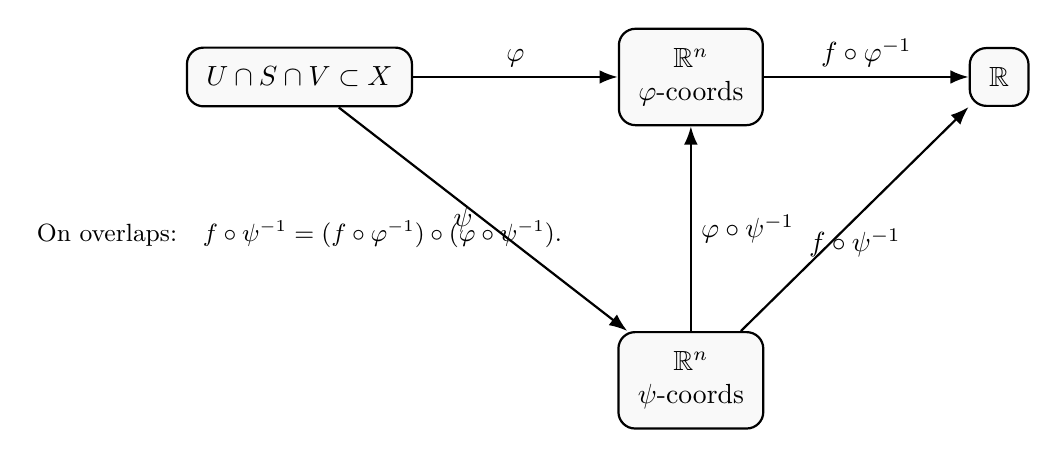
\begin{tikzpicture}[>=Latex, node distance=26mm and 26mm]
		\tikzset{
			box/.style={rounded corners=6pt, draw=black, thick, fill=gray!5, inner sep=7pt, align=center},
			arr/.style={->, thick},
		}
		\node[box] (X) {$U\cap S\cap V \subset X$};
		\node[box, right=of X] (R) {$\mathbb{R}^n$\\$\varphi$-coords};
		\node[box, below=of R] (R2) {$\mathbb{R}^n$\\$\psi$-coords};
		\node[box, right=of R] (reals) {$\mathbb{R}$};
		
		\draw[arr] (X) -- node[above] {$\varphi$} (R);
		\draw[arr] (X) -- node[left] {$\psi$} (R2);
		\draw[arr] (R) -- node[above] {$f\circ\varphi^{-1}$} (reals);
		\draw[arr] (R2) -- node[below] {$f\circ\psi^{-1}$} (reals);
		\draw[arr] (R2) -- node[right] {$\varphi\circ\psi^{-1}$} (R);
		
		\node[align=left] at ($(X)+(0,-2.0)$) {\small On overlaps:\quad $f\circ\psi^{-1}=(f\circ\varphi^{-1})\circ(\varphi\circ\psi^{-1})$.};
	\end{tikzpicture}
	\caption{Smooth compatibility transfers smoothness of $f$ between atlases.}
\end{figure}


% ---------- Figure 2 (improved): Converse via coordinate functions ----------
\begin{figure}[H]
	\centering
	
	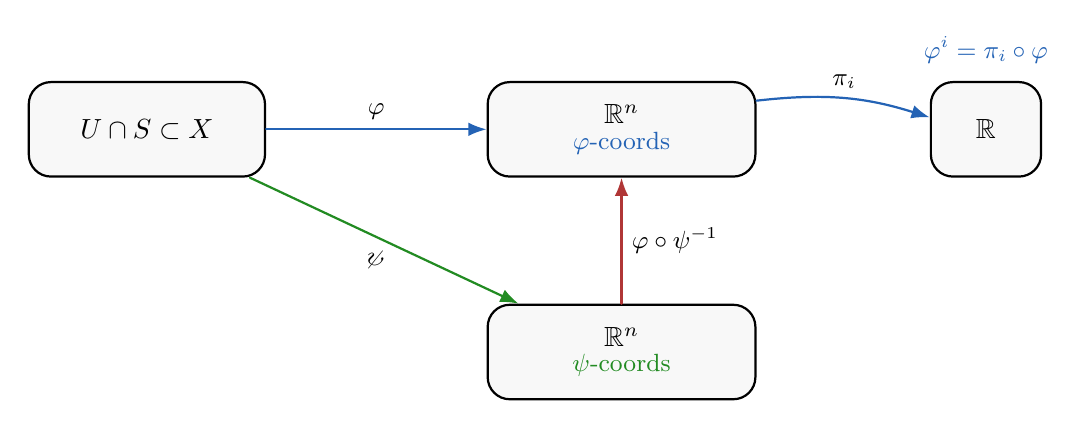
\begin{tikzpicture}[>=Latex, line cap=round, line join=round,
		node distance=22mm and 28mm]
		
		% Colors
		\definecolor{PhiBlue}{RGB}{36,99,181}
		\definecolor{PsiGreen}{RGB}{34,139,34}
		\definecolor{TransRed}{RGB}{176,54,54}
		\definecolor{BoxFill}{RGB}{248,248,248}
		
		% Styles (fixed widths!)
		\tikzset{
			box/.style={
				rounded corners=8pt, draw=black, thick, fill=BoxFill,
				inner sep=7pt, align=center, minimum height=12mm
			},
			wide/.style={box, minimum width=34mm},
			mid/.style={box, minimum width=30mm},
			small/.style={box, minimum width=14mm},
			arrPhi/.style={->, thick, draw=PhiBlue},
			arrPsi/.style={->, thick, draw=PsiGreen},
			arrTrans/.style={->, thick, draw=TransRed},
			lbl/.style={font=\small}
		}
		
		% Nodes
		\node[mid] (X) {$U\cap S\subset X$};
		
		\node[wide, right=of X] (RnPhi)
		{$\mathbb R^n$\\[-1mm]\textcolor{PhiBlue}{\small $\varphi$-coords}};
		
		\node[wide, below=16mm of RnPhi] (RnPsi)
		{$\mathbb R^n$\\[-1mm]\textcolor{PsiGreen}{\small $\psi$-coords}};
		
		\node[small, right=22mm of RnPhi] (R) {$\mathbb R$};
		
		% Arrows (NO arrow crosses text)
		\draw[arrPhi] (X) -- node[above, lbl] {$\varphi$} (RnPhi);
		\draw[arrPsi] (X) -- node[sloped, below, lbl] {$\psi$} (RnPsi);
		
		\draw[arrTrans] (RnPsi) -- node[right, lbl] {$\varphi\circ\psi^{-1}$} (RnPhi);
		
		\draw[arrPhi] (RnPhi) to[bend left=12] node[above, lbl] {$\pi_i$} (R);
		\node[lbl, above=1mm of R] {\textcolor{PhiBlue}{$\varphi^i=\pi_i\circ\varphi$}};
		
	\end{tikzpicture}
	
	\caption{Converse: coordinate functions force transition smoothness.}
	
	\vspace{0.5em}
	\noindent\textbf{Key idea (with dimensions).}
	The charts have types $\varphi:U\to\mathbb R^n$ and $\psi:S\to\mathbb R^n$, hence
	$\varphi\circ\psi^{-1}:\psi(U\cap S)\to\varphi(U\cap S)\subset\mathbb R^n$.
	Writing $\varphi=(\varphi^1,\dots,\varphi^n)$ with $\varphi^i:U\to\mathbb R$, we have
	$\varphi^i\circ\psi^{-1}:\psi(U\cap S)\to\mathbb R$.
	A map into $\mathbb R^n$ is smooth iff all its components are smooth, so smoothness of every
	$\varphi^i\circ\psi^{-1}$ implies smoothness of $\varphi\circ\psi^{-1}$.
\end{figure}

\noindent\textbf{Figure explanation.}
Assume the class of $\mathcal A$-smooth real-valued functions equals the class of $\mathcal B$-smooth ones on every open set.
For a chart $(U,\varphi)\in\mathcal A$, each coordinate function $\varphi^i:U\to\mathbb R$ is $\mathcal A$-smooth, hence also $\mathcal B$-smooth.
Therefore $\varphi^i\circ\psi^{-1}$ is smooth on $\psi(U\cap S)$ for every overlapping $(S,\psi)\in\mathcal B$.
Since $\varphi\circ\psi^{-1}=(\varphi^1\circ\psi^{-1},\dots,\varphi^n\circ\psi^{-1})$, the transition map is smooth.


\begin{figure}[H]
	\centering
	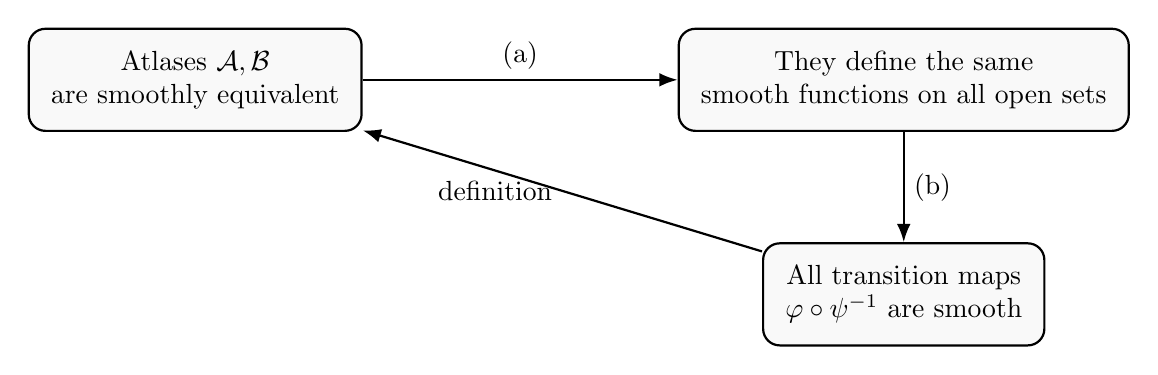
\begin{tikzpicture}[>=Latex]
		\tikzset{
			box/.style={rounded corners=6pt, draw=black, thick, fill=gray!5, inner sep=8pt, align=center},
			arr/.style={->, thick},
		}
		\node[box] (eq) {Atlases $\mathcal A,\mathcal B$\\ are smoothly equivalent};
		\node[box, right=40mm of eq] (sf) {They define the same\\ smooth functions on all open sets};
		\node[box, below=14mm of sf] (trans) {All transition maps\\ $\varphi\circ\psi^{-1}$ are smooth};
		
		\draw[arr] (eq) -- node[above] {(a)} (sf);
		\draw[arr] (sf) -- node[right] {(b)} (trans);
		\draw[arr] (trans) -- node[left] {definition} (eq);
		
	\end{tikzpicture}
	\caption{Logic of Problem 1: equivalence of atlases is the same as agreeing on smooth functions.}
\end{figure}



% ============================================================
% Theory: Problem 1
% ============================================================

\subsection*{Theory for Problem 1 (Atlases, smooth equivalence, smooth functions)}

\paragraph{Charts and atlases.}
A \emph{chart} on a topological $n$-manifold $X$ is a homeomorphism
\[
\varphi:U\longrightarrow V\subset \mathbb R^n
\]
where $U\subset X$ is open and $V\subset\mathbb R^n$ is open.
An \emph{atlas} $\mathcal A$ is a collection of charts whose domains cover $X$.

\paragraph{Smooth compatibility and smooth atlases.}
Two charts $(U,\varphi)$ and $(S,\psi)$ are \emph{smoothly compatible} if the transition maps
\[
\varphi\circ \psi^{-1}:\psi(U\cap S)\to \varphi(U\cap S),
\qquad
\psi\circ \varphi^{-1}:\varphi(U\cap S)\to \psi(U\cap S)
\]
are $C^\infty$ maps between open subsets of $\mathbb R^n$.
An atlas is a \emph{smooth atlas} if every pair of its charts is smoothly compatible.

\paragraph{Smooth equivalence of atlases.}
Two smooth atlases $\mathcal A$ and $\mathcal B$ are \emph{smoothly equivalent} if every chart in $\mathcal A$
is smoothly compatible with every chart in $\mathcal B$.
Equivalently, $\mathcal A\cup\mathcal B$ is again a smooth atlas.

\paragraph{Smooth functions defined by an atlas.}
Given an atlas $\mathcal A$, a function $f:U\to\mathbb R$ (with $U\subset X$ open) is \emph{$\mathcal A$-smooth}
if for every chart $(V,\varphi)\in\mathcal A$ the coordinate expression
\[
f\circ \varphi^{-1}:\varphi(U\cap V)\to \mathbb R
\]
is smooth in the usual Euclidean sense.

\paragraph{Componentwise smoothness.}
A map $g=(g^1,\dots,g^n):W\subset\mathbb R^m\to\mathbb R^n$ is smooth if and only if each component
$g^i:W\to\mathbb R$ is smooth. This is the basic tool used to recover smoothness of a transition map from smoothness of
its coordinate components.

\paragraph{Coordinate functions.}
If $\varphi:U\to\mathbb R^n$ is a chart, write $\varphi=(\varphi^1,\dots,\varphi^n)$ with
coordinate functions $\varphi^i:U\to\mathbb R$.
In $\varphi$-coordinates, $\varphi^i$ becomes the standard projection $\pi_i:\mathbb R^n\to\mathbb R$,
so each $\varphi^i$ is automatically smooth with respect to any atlas containing $\varphi$.




% ============================================================
% Problem 2
% ============================================================

\subsection*{Problem 2: Homogeneous coordinate charts on $\mathbb{RP}^n$ and $\mathbb{CP}^n$}

\noindent\textbf{Problem statement.}
Show that the homogeneous coordinate maps on $\mathbb{RP}^n$ and $\mathbb{CP}^n$ define smooth pseudo-atlases.
Show that the resulting spaces are Hausdorff and second-countable, hence are smooth manifolds.

\medskip
\noindent\textbf{Solution.}

\smallskip
\noindent\textbf{(A) $\mathbb{RP}^n$.}
Recall $\mathbb{RP}^n$ consists of lines through $0$ in $\mathbb R^{n+1}$; write points as
$[x_0:\cdots:x_n]$ with $(x_0,\dots,x_n)\neq 0$ and $[x]=[\lambda x]$ for $\lambda\neq 0$.
For $i=0,\dots,n$ define
\[
U_i=\{[x_0:\cdots:x_n]\in\mathbb{RP}^n:\ x_i\neq 0\}.
\]
Define $\phi_i:U_i\to\mathbb R^n$ by
\[
\phi_i([x_0:\cdots:x_n])
=
\Big(\frac{x_0}{x_i},\dots,\frac{x_{i-1}}{x_i},\frac{x_{i+1}}{x_i},\dots,\frac{x_n}{x_i}\Big).
\]
This is well-defined since scaling cancels in the ratios. It is a bijection onto $\mathbb R^n$ with inverse
sending $y\in\mathbb R^n$ to the class with $i$-th coordinate $1$ and the remaining coordinates given by $y$.

On overlaps $U_i\cap U_j$, the transition maps $\phi_j\circ\phi_i^{-1}$ are given by rational expressions
(with denominators nonzero exactly on the overlap), hence are smooth. Therefore the homogeneous charts define a smooth atlas.

\smallskip
\noindent\textbf{(B) $\mathbb{CP}^n$.}
Similarly, points are complex lines in $\mathbb C^{n+1}$, written $[z_0:\cdots:z_n]$ with $[z]=[\lambda z]$, $\lambda\in\mathbb C^\times$.
Let
\[
V_i=\{[z_0:\cdots:z_n]\in\mathbb{CP}^n:\ z_i\neq 0\},
\qquad
\Phi_i:V_i\to\mathbb C^n
\]
be defined by
\[
\Phi_i([z_0:\cdots:z_n])
=
\Big(\frac{z_0}{z_i},\dots,\frac{z_{i-1}}{z_i},\frac{z_{i+1}}{z_i},\dots,\frac{z_n}{z_i}\Big).
\]
Transition maps are again rational in the complex coordinates, hence holomorphic on overlaps and therefore smooth
when we identify $\mathbb C^n\cong\mathbb R^{2n}$. Thus $\mathbb{CP}^n$ becomes a smooth manifold of real dimension $2n$.

\smallskip
\noindent\textbf{(C) Hausdorff and second-countable.}
Give $\mathbb{RP}^n$ (resp.\ $\mathbb{CP}^n$) the topology for which each chart map is a homeomorphism onto an open subset of $\mathbb R^n$
(resp.\ $\mathbb R^{2n}$): a set $O$ is open iff $\phi_i(O\cap U_i)$ is open for all $i$ (resp.\ $\Phi_i(O\cap V_i)$).

\begin{itemize}
	\item \emph{Hausdorff:} if two points lie in a common chart domain, separate their images in $\mathbb R^n$ (or $\mathbb R^{2n}$) by disjoint open sets
	and pull back. If they do not lie in a common chart domain, one can still separate using chart domains and their complements.
	\item \emph{Second-countable:} $\mathbb R^n$ has a countable basis $\mathcal B$. Then
	$\{\phi_i^{-1}(B): B\in\mathcal B,\ i=0,\dots,n\}$ is a countable basis (finite index set $\times$ countable set is countable).
\end{itemize}
Hence $\mathbb{RP}^n$ is a smooth $n$-manifold and $\mathbb{CP}^n$ is a smooth $2n$-manifold.

\medskip
\noindent\textbf{Examples.}
\begin{itemize}
	\item $\mathbb{RP}^1$ is a smooth $1$-manifold (in fact diffeomorphic to $S^1$).
	\item $\mathbb{CP}^1$ is a smooth $2$-manifold (in fact diffeomorphic to $S^2$, the Riemann sphere).
	\item In $\mathbb{RP}^2$, the transition between $\phi_0$ and $\phi_1$ has the form $(u,v)\mapsto (1/u,\,v/u)$ on the domain $u\neq 0$,
	hence is smooth on its overlap domain.
\end{itemize}


% ============================================================
% Problem 3
% ============================================================

\subsection*{Problem 3: Local chart criterion for smoothness of a map}

\noindent\textbf{Problem statement.}
Let $X,Y$ be smooth manifolds with atlases
\[
\{\varphi_\alpha:U_\alpha\to V_\alpha\}_{\alpha\in A},
\qquad
\{\psi_\beta:S_\beta\to T_\beta\}_{\beta\in B}.
\]
Show that a map $F:X\to Y$ is smooth if and only if there exists a cover $\{W_\gamma\}_{\gamma\in C}$ of $X$ and
for each $\gamma$ there exist $\alpha(\gamma)\in A$ and $\beta(\gamma)\in B$ such that:
\begin{enumerate}
	\item[(a)] $W_\gamma\subset U_{\alpha(\gamma)}$ and $F(W_\gamma)\subset S_{\beta(\gamma)}$,
	\item[(b)] $\varphi_{\alpha(\gamma)}(W_\gamma)$ is open in $V_{\alpha(\gamma)}$,
	\item[(c)] the map
	\[
	\psi_{\beta(\gamma)}\circ F\circ \big(\varphi_{\alpha(\gamma)}\vert_{W_\gamma}\big)^{-1}
	:\ \varphi_{\alpha(\gamma)}(W_\gamma)\longrightarrow T_{\beta(\gamma)}
	\]
	is smooth.
\end{enumerate}

\medskip
\noindent\textbf{Solution.}

\smallskip
\noindent\textbf{($\Rightarrow$)}
Assume $F$ is smooth. For each $x\in X$, by the definition of smoothness choose charts
$(U_\alpha,\varphi_\alpha)$ around $x$ and $(S_\beta,\psi_\beta)$ around $F(x)$ such that
$\psi_\beta\circ F\circ\varphi_\alpha^{-1}$ is smooth on a neighborhood of $\varphi_\alpha(x)$.
Shrink to an open neighborhood $W_x\subset U_\alpha$ with $x\in W_x$, $F(W_x)\subset S_\beta$,
and $\varphi_\alpha(W_x)$ open, so that
\[
\psi_\beta\circ F\circ(\varphi_\alpha\vert_{W_x})^{-1}
\]
is smooth on $\varphi_\alpha(W_x)$. The sets $\{W_x\}_{x\in X}$ form an open cover; relabel by $\gamma$.

\smallskip
\noindent\textbf{($\Leftarrow$)}
Conversely assume such a cover $\{W_\gamma\}$ exists with smooth coordinate expressions in the chosen charts.
To prove $F$ is smooth in the usual sense, let $x\in X$ and choose arbitrary charts $(U,\varphi)$ about $x$
and $(S,\psi)$ about $F(x)$. Pick $\gamma$ with $x\in W_\gamma$.
On $\varphi(W_\gamma\cap U)$ we can write
\[
\psi\circ F\circ\varphi^{-1}
=
(\psi\circ\psi_{\beta(\gamma)}^{-1})
\circ
(\psi_{\beta(\gamma)}\circ F\circ\varphi_{\alpha(\gamma)}^{-1})
\circ
(\varphi_{\alpha(\gamma)}\circ\varphi^{-1}).
\]
The middle map is smooth by assumption (on the appropriate domain),
and the left/right maps are transition maps between charts in $Y$ and $X$, hence smooth.
Therefore $\psi\circ F\circ\varphi^{-1}$ is smooth near $\varphi(x)$.
Since $x$ was arbitrary, $F$ is smooth.

\medskip
\noindent\textbf{Examples.}
\begin{itemize}
	\item \emph{Inclusion $S^n\hookrightarrow\mathbb R^{n+1}$.}
	Using stereographic charts on $S^n$ and the standard chart on $\mathbb R^{n+1}$,
	the coordinate expression of the inclusion is smooth on each chart domain; hence the inclusion is smooth.
	\item \emph{Projective map induced by a linear map.}
	If $A:\mathbb R^{n+1}\to\mathbb R^{n+1}$ is invertible, then $F([x])=[Ax]$ defines $F:\mathbb{RP}^n\to\mathbb{RP}^n$.
	In homogeneous charts $U_i$, the coordinate formulas are quotients of linear functions (rational with nonzero denominators on overlaps),
	hence smooth; the cover criterion applies.
	\item \emph{Stereographic projection.}
	The stereographic map $S^2\setminus\{N\}\to\mathbb R^2$ is smooth because its coordinate formula is smooth on its domain.
\end{itemize}

% ============================================================
% Theory: Problem 2
% ============================================================

\subsection*{Theory for Problem 2 (Homogeneous coordinates and projective manifolds)}

\paragraph{Projective space as a quotient.}
Real projective space is the quotient
\[
\mathbb{RP}^n = (\mathbb R^{n+1}\setminus\{0\})/\sim,
\qquad
x\sim \lambda x \ \ (\lambda\in\mathbb R^\times),
\]
and complex projective space is
\[
\mathbb{CP}^n = (\mathbb C^{n+1}\setminus\{0\})/\sim,
\qquad
z\sim \lambda z \ \ (\lambda\in\mathbb C^\times).
\]
Elements are written in \emph{homogeneous coordinates} as $[x_0:\cdots:x_n]$ or $[z_0:\cdots:z_n]$.

\paragraph{Standard chart domains.}
For each $i=0,\dots,n$ define
\[
U_i=\{[x]\in\mathbb{RP}^n: x_i\neq 0\},
\qquad
V_i=\{[z]\in\mathbb{CP}^n: z_i\neq 0\}.
\]
These sets cover $\mathbb{RP}^n$ and $\mathbb{CP}^n$, respectively.

\paragraph{Homogeneous coordinate charts.}
Define charts
\[
\phi_i:U_i\to\mathbb R^n,
\qquad
\phi_i([x_0:\cdots:x_n])=
\Big(\frac{x_0}{x_i},\dots,\widehat{\frac{x_i}{x_i}},\dots,\frac{x_n}{x_i}\Big),
\]
where the hat means the $i$-th slot is omitted.
Similarly,
\[
\Phi_i:V_i\to\mathbb C^n,
\qquad
\Phi_i([z_0:\cdots:z_n])=
\Big(\frac{z_0}{z_i},\dots,\widehat{\frac{z_i}{z_i}},\dots,\frac{z_n}{z_i}\Big).
\]
These maps are well-defined because scaling by $\lambda$ cancels in the ratios.

\paragraph{Transition maps are rational.}
On overlaps $U_i\cap U_j$, the transition functions $\phi_j\circ\phi_i^{-1}$ are given by rational expressions
whose denominators are nonzero on the overlap, hence are smooth.
On overlaps $V_i\cap V_j$, the transition functions $\Phi_j\circ\Phi_i^{-1}$ are holomorphic (rational),
and therefore smooth when we identify $\mathbb C^n\cong \mathbb R^{2n}$.

\paragraph{Topology, Hausdorffness, and second-countability.}
Declare $O\subset\mathbb{RP}^n$ open iff $\phi_i(O\cap U_i)$ is open in $\mathbb R^n$ for all $i$
(and similarly for $\mathbb{CP}^n$ using $\Phi_i$).
With this topology:
\begin{itemize}
	\item $\mathbb{RP}^n$ and $\mathbb{CP}^n$ are Hausdorff since points can be separated inside a common chart by disjoint Euclidean open sets.
	\item They are second-countable: if $\mathcal B$ is a countable basis of $\mathbb R^n$ (resp.\ $\mathbb R^{2n}$), then
	$\{\phi_i^{-1}(B):B\in\mathcal B,\ i=0,\dots,n\}$ (resp.\ $\{\Phi_i^{-1}(B)\}$) is a countable basis.
\end{itemize}
Hence the homogeneous coordinate pseudo-atlases define smooth manifolds with
\[
\dim(\mathbb{RP}^n)=n,
\qquad
\dim_{\mathbb R}(\mathbb{CP}^n)=2n.
\]

% ============================================================
% Problem 3
% ============================================================

\subsection*{Problem 3: Local chart criterion for smoothness of a map}

\noindent\textbf{Problem statement.}
Let $X,Y$ be smooth manifolds with atlases
\[
\{\varphi_\alpha:U_\alpha\to V_\alpha\}_{\alpha\in A},
\qquad
\{\psi_\beta:S_\beta\to T_\beta\}_{\beta\in B}.
\]
Show that a map $F:X\to Y$ is smooth if and only if there exists a cover $\{W_\gamma\}_{\gamma\in C}$ of $X$ and
for each $\gamma$ there exist $\alpha(\gamma)\in A$ and $\beta(\gamma)\in B$ such that:
\begin{enumerate}
	\item[(a)] $W_\gamma\subset U_{\alpha(\gamma)}$ and $F(W_\gamma)\subset S_{\beta(\gamma)}$,
	\item[(b)] $\varphi_{\alpha(\gamma)}(W_\gamma)$ is open in $V_{\alpha(\gamma)}$,
	\item[(c)] the map
	\[
	\psi_{\beta(\gamma)}\circ F\circ \big(\varphi_{\alpha(\gamma)}\vert_{W_\gamma}\big)^{-1}
	:\ \varphi_{\alpha(\gamma)}(W_\gamma)\longrightarrow T_{\beta(\gamma)}
	\]
	is smooth.
\end{enumerate}

\medskip
\noindent\textbf{Solution.}

\smallskip
\noindent\textbf{($\Rightarrow$)}
Assume $F$ is smooth. For each $x\in X$, by the definition of smoothness choose charts
$(U_\alpha,\varphi_\alpha)$ around $x$ and $(S_\beta,\psi_\beta)$ around $F(x)$ such that
$\psi_\beta\circ F\circ\varphi_\alpha^{-1}$ is smooth on a neighborhood of $\varphi_\alpha(x)$.
Shrink to an open neighborhood $W_x\subset U_\alpha$ with $x\in W_x$, $F(W_x)\subset S_\beta$,
and $\varphi_\alpha(W_x)$ open, so that
\[
\psi_\beta\circ F\circ(\varphi_\alpha\vert_{W_x})^{-1}
\]
is smooth on $\varphi_\alpha(W_x)$. The sets $\{W_x\}_{x\in X}$ form an open cover; relabel by $\gamma$.

\smallskip
\noindent\textbf{($\Leftarrow$)}
Conversely assume such a cover $\{W_\gamma\}$ exists with smooth coordinate expressions in the chosen charts.
To prove $F$ is smooth in the usual sense, let $x\in X$ and choose arbitrary charts $(U,\varphi)$ about $x$
and $(S,\psi)$ about $F(x)$. Pick $\gamma$ with $x\in W_\gamma$.
On $\varphi(W_\gamma\cap U)$ we can write
\[
\psi\circ F\circ\varphi^{-1}
=
(\psi\circ\psi_{\beta(\gamma)}^{-1})
\circ
(\psi_{\beta(\gamma)}\circ F\circ\varphi_{\alpha(\gamma)}^{-1})
\circ
(\varphi_{\alpha(\gamma)}\circ\varphi^{-1}).
\]
The middle map is smooth by assumption (on the appropriate domain),
and the left/right maps are transition maps between charts in $Y$ and $X$, hence smooth.
Therefore $\psi\circ F\circ\varphi^{-1}$ is smooth near $\varphi(x)$.
Since $x$ was arbitrary, $F$ is smooth.

\medskip
\noindent\textbf{Examples.}
\begin{itemize}
	\item \emph{Inclusion $S^n\hookrightarrow\mathbb R^{n+1}$.}
	Using stereographic charts on $S^n$ and the standard chart on $\mathbb R^{n+1}$,
	the coordinate expression of the inclusion is smooth on each chart domain; hence the inclusion is smooth.
	\item \emph{Projective map induced by a linear map.}
	If $A:\mathbb R^{n+1}\to\mathbb R^{n+1}$ is invertible, then $F([x])=[Ax]$ defines $F:\mathbb{RP}^n\to\mathbb{RP}^n$.
	In homogeneous charts $U_i$, the coordinate formulas are quotients of linear functions (rational with nonzero denominators on overlaps),
	hence smooth; the cover criterion applies.
	\item \emph{Stereographic projection.}
	The stereographic map $S^2\setminus\{N\}\to\mathbb R^2$ is smooth because its coordinate formula is smooth on its domain.
\end{itemize}

% ============================================================
% Theory: Problem 3
% ============================================================

\subsection*{Theory for Problem 3 (Local chart criterion for smooth maps)}

\paragraph{Smooth maps via coordinate expressions.}
Let $X$ and $Y$ be smooth manifolds and let $F:X\to Y$ be a map.
The map $F$ is \emph{smooth at} $x\in X$ if for (equivalently, any) charts $(U,\varphi)$ about $x$
and $(S,\psi)$ about $F(x)$, the coordinate representative
\[
\psi\circ F\circ \varphi^{-1}:\ \varphi\!\big(U\cap F^{-1}(S)\big)\longrightarrow \psi(S)
\]
is a smooth map between open subsets of Euclidean spaces.
The map $F$ is \emph{smooth} if it is smooth at every point.

\paragraph{Smoothness is local.}
Smoothness depends only on the behavior of $F$ on neighborhoods:
if $\{W_\gamma\}$ is an open cover of $X$ and each restriction $F|_{W_\gamma}$ is smooth,
then $F$ is smooth on $X$.

\paragraph{Checking smoothness on a cover using charts.}
To verify smoothness it suffices to cover $X$ by sets $W_\gamma$ and choose, for each $\gamma$,
charts $(U_{\alpha(\gamma)},\varphi_{\alpha(\gamma)})$ on $X$ and $(S_{\beta(\gamma)},\psi_{\beta(\gamma)})$ on $Y$
such that
\[
W_\gamma\subset U_{\alpha(\gamma)},\qquad F(W_\gamma)\subset S_{\beta(\gamma)},
\qquad \varphi_{\alpha(\gamma)}(W_\gamma)\ \text{is open},
\]
and the coordinate expression
\[
\psi_{\beta(\gamma)}\circ F\circ \big(\varphi_{\alpha(\gamma)}|_{W_\gamma}\big)^{-1}:
\varphi_{\alpha(\gamma)}(W_\gamma)\to T_{\beta(\gamma)}
\]
is smooth. This is precisely the local-chart criterion formulated in Problem~3.

\paragraph{Why the ``open image'' condition appears.}
A Euclidean $C^\infty$-map is defined on an open set in $\mathbb R^n$.
Since charts are homeomorphisms, the condition that $\varphi_{\alpha(\gamma)}(W_\gamma)$ is open
is equivalent to $W_\gamma$ being open in $X$, but phrasing it in coordinates avoids mentioning the topology explicitly.

\paragraph{Transition-map factorization (change of charts).}
If $(U,\varphi)$ and $(U_{\alpha},\varphi_{\alpha})$ are charts on $X$ and
$(S,\psi)$ and $(S_{\beta},\psi_{\beta})$ are charts on $Y$, then on the appropriate domain one has
\[
\psi\circ F\circ \varphi^{-1}
=
(\psi\circ \psi_{\beta}^{-1})
\circ
(\psi_{\beta}\circ F\circ \varphi_{\alpha}^{-1})
\circ
(\varphi_{\alpha}\circ \varphi^{-1}).
\]
Thus, if one coordinate representative is smooth and the transition maps are smooth
(by compatibility of the atlases), then every other coordinate representative is smooth.
This is the mechanism behind the cover-based smoothness test in Problem~3.

% ============================================================
% Next problems: 4--7 (statements)
% ============================================================

\subsection*{Problem 4: Smoothness of the Hopf map}

\noindent\textbf{Problem statement.}
Using the local-chart criterion from \textbf{Problem 3}, show that the Hopf map
\[
H:S^{2n+1}\longrightarrow \mathbb{CP}^n
\]
is smooth.

% ============================================================
% Theory: Problem 4 (Hopf map)
% ============================================================

\subsection*{Theory for Problem 4 (The Hopf map)}

\paragraph{Definition of the Hopf map.}
View $S^{2n+1}\subset\mathbb C^{n+1}$ as
\[
S^{2n+1}=\Big\{z=(z_0,\dots,z_n)\in\mathbb C^{n+1}:\ \|z\|^2=\sum_{k=0}^n |z_k|^2=1\Big\}.
\]
The \emph{Hopf map} is
\[
H:S^{2n+1}\longrightarrow \mathbb{CP}^n,
\qquad
H(z)=[z_0:\cdots:z_n].
\]
Its fibers are the $S^1$-orbits of the action $e^{i\theta}\cdot z=(e^{i\theta}z_0,\dots,e^{i\theta}z_n)$.

\paragraph{Standard projective charts.}
For each $j=0,\dots,n$ let
\[
U_j=\{[w]\in\mathbb{CP}^n:\ w_j\neq 0\}.
\]
The standard homogeneous-coordinate chart is
\[
\Phi_j:U_j\to \mathbb C^n,\qquad
\Phi_j([w_0:\cdots:w_n])=
\Big(\frac{w_0}{w_j},\dots,\widehat{\frac{w_j}{w_j}},\dots,\frac{w_n}{w_j}\Big),
\]
where the hat indicates that the $j$-th entry is omitted.

\paragraph{Local coordinate expression of $H$.}
Define
\[
W_j:=H^{-1}(U_j)=\{z\in S^{2n+1}:\ z_j\neq 0\}.
\]
Then $W_j$ is open in $S^{2n+1}$ and $\{W_j\}_{j=0}^n$ covers $S^{2n+1}$.
On $W_j$ the coordinate representative of $H$ is
\[
\Phi_j\circ H\big|_{W_j}:W_j\to\mathbb C^n,
\qquad
z\longmapsto
\Big(\frac{z_0}{z_j},\dots,\widehat{\frac{z_j}{z_j}},\dots,\frac{z_n}{z_j}\Big).
\]

\paragraph{Smoothness mechanism (link to Problem 3).}
Each component $z\mapsto z_k/z_j$ is a smooth (indeed holomorphic) function on the Euclidean open set
$\{z_j\neq 0\}\subset\mathbb C^{n+1}\cong\mathbb R^{2n+2}$, and restricting to the submanifold $S^{2n+1}$ preserves smoothness.
Hence $\Phi_j\circ H|_{W_j}$ is smooth for each $j$.
By the cover-based criterion of Problem~3, this implies that $H$ is a smooth map $S^{2n+1}\to\mathbb{CP}^n$.

\paragraph{Fiber picture (Hopf fibration).}
Fix $[w]\in\mathbb{CP}^n$ and choose a representative $w\in\mathbb C^{n+1}\setminus\{0\}$.
Normalize to unit length $\hat w=w/\|w\|\in S^{2n+1}$.
Then the fiber of $H$ over $[w]$ is the $S^1$-orbit through $\hat w$:
\[
H^{-1}([w])=\{e^{i\theta}\hat w:\theta\in\mathbb R\}\cong S^1.
\]
Indeed $H(e^{i\theta}\hat w)=[e^{i\theta}\hat w]=[\hat w]=[w]$, and if $z\in S^{2n+1}$ satisfies $H(z)=[w]$
then $z=\lambda \hat w$ for some $\lambda\in\mathbb C^\times$; the unit-length condition gives $|\lambda|=1$,
so $\lambda=e^{i\theta}$.
Thus $H$ is the quotient map for the free $S^1$-action $e^{i\theta}\cdot z=(e^{i\theta}z_0,\dots,e^{i\theta}z_n)$ on $S^{2n+1}$.


% ------------------------------------------------------------

\subsection*{Problem 5: When $(x,r)$ are local coordinates in $\mathbb R^2$}

\noindent\textbf{Problem statement.}
Consider the functions on $\mathbb R^2$
\[
x(x,y)=x,\qquad r(x,y)=\sqrt{x^2+y^2}.
\]
About which points of $\mathbb R^2$ do the functions $x$ and $r$ provide local coordinates?
Equivalently: for which points can we use $(x,r)$ as a chart?
Draw the corresponding basis vectors $\partial_x$ and $\partial_r$ at a representative selection of points.



\paragraph{\textbf{Solution.}}
Consider
\[
\Phi:\mathbb{R}^2\to \mathbb{R}^2,\qquad \Phi(x,y)=(x,r),\quad r(x,y)=\sqrt{x^2+y^2}.
\]
The pair $(x,r)$ gives a local coordinate chart precisely at points where $\Phi$ is a local diffeomorphism,
i.e.\ where $\det D\Phi\neq 0$ (and where $r$ is smooth).

\paragraph{Where is $(x,r)$ a chart?}
For $r>0$ we have
\[
D\Phi(x,y)=
\begin{pmatrix}
	\partial_x x & \partial_y x\\[2pt]
	\partial_x r & \partial_y r
\end{pmatrix}
=
\begin{pmatrix}
	1 & 0\\[2pt]
	\frac{x}{r} & \frac{y}{r}
\end{pmatrix},
\qquad
\det D\Phi(x,y)=\frac{y}{r}.
\]
Hence $\det D\Phi\neq 0$ iff $y\neq 0$ (and then automatically $r>0$). Therefore $(x,r)$ are local
coordinates at exactly the points of $\mathbb{R}^2$ with $y\neq 0$, i.e.\ on the upper and lower half-planes.
They fail on the $x$-axis ($y=0$), and at the origin $r$ is not smooth so it cannot be used as a coordinate.

Moreover, the inverse relation is $y=\pm\sqrt{r^2-x^2}$, so $(x,r)$ defines a chart on each connected component
$y>0$ and $y<0$ separately.

\paragraph{Coordinate basis vectors $\partial_x$ and $\partial_r$.}
Fix one branch (either $y>0$ or $y<0$), so locally
\[
(x,r)\longmapsto (x,y(x,r)),\qquad y=\pm\sqrt{r^2-x^2}.
\]
Then
\[
\left(\frac{\partial y}{\partial x}\right)_{r}=-\frac{x}{y},
\qquad
\left(\frac{\partial y}{\partial r}\right)_{x}=\frac{r}{y}.
\]
Thus, as vectors in the standard $(x,y)$-coordinates,
\[
\boxed{\;\partial_x\Big|_{r}=(1,-x/y)\;},\qquad
\boxed{\;\partial_r\Big|_{x}=(0,r/y)\;}
\qquad (y\neq 0).
\]
Geometrically, $\partial_r|_x$ points vertically (up on $y>0$, down on $y<0$), while
$\partial_x|_r$ is tangent to the circle $x^2+y^2=r^2$ in the direction of increasing $x$.


% ============================================================
% Theory: Problem 5
% ============================================================

\subsection*{Theory for Problem 5 ($(x,r)$ as local coordinates in $\mathbb R^2$)}

\paragraph{The coordinate map.}
Consider
\[
F:\mathbb R^2\to\mathbb R^2,\qquad F(x,y)=(x,r)=(x,\sqrt{x^2+y^2}).
\]
Saying that $(x,r)$ provide local coordinates near $p=(x_0,y_0)$ means that $F$ is a local diffeomorphism at $p$
(i.e.\ $F$ restricts to a diffeomorphism from some neighborhood of $p$ onto an open subset of $\mathbb R^2$).

\paragraph{Inverse Function Theorem criterion.}
For $r=\sqrt{x^2+y^2}$ one has, when $r\neq 0$,
\[
\frac{\partial r}{\partial x}=\frac{x}{r},
\qquad
\frac{\partial r}{\partial y}=\frac{y}{r}.
\]
Hence
\[
DF(x,y)=
\begin{pmatrix}
	1 & 0\\[2pt]
	\frac{x}{r} & \frac{y}{r}
\end{pmatrix}
\quad (r\neq 0),
\qquad
\det DF(x,y)=\frac{y}{r}.
\]
Therefore $\det DF(p)\neq 0$ holds exactly when $y\neq 0$.
In particular, $(x,r)$ fails on the $x$-axis ($y=0$), and also at the origin where $r=0$ and the derivatives are not defined.

\paragraph{Geometric interpretation.}
For fixed $(x,r)$ with $r>|x|$, there are typically two points
\[
(x,y)=\big(x,\pm\sqrt{r^2-x^2}\big),
\]
so $(x,r)$ cannot distinguish the upper and lower half-planes.
Restricting to $y>0$ or $y<0$ removes this ambiguity and yields valid local coordinates.

\paragraph{Coordinate basis vectors.}
On the region $y>0$ (resp.\ $y<0$) we may write the inverse as
\[
x=x,\qquad y=\pm\sqrt{r^2-x^2}.
\]
Thus the coordinate vector fields in $(x,r)$-coordinates are
\[
\partial_x=\Big(1,\ \frac{\partial y}{\partial x}\Big)
=\Big(1,\ \mp\frac{x}{\sqrt{r^2-x^2}}\Big),
\qquad
\partial_r=\Big(0,\ \frac{\partial y}{\partial r}\Big)
=\Big(0,\ \pm\frac{r}{\sqrt{r^2-x^2}}\Big),
\]
with the upper sign for $y>0$ and the lower sign for $y<0$.
Geometrically, $\partial_x$ is tangent to the circle $r=\mathrm{const}$, while $\partial_r$ changes the radius at fixed $x$.


% ------------------------------------------------------------

\subsection*{Problem 6: Smooth homeomorphism of $\mathbb R$ that is not a diffeomorphism}

\noindent\textbf{Problem statement.}
Write down a smooth homeomorphism
\[
f:\mathbb R\longrightarrow \mathbb R
\]
that is not a diffeomorphism.

% ============================================================
% Theory for Problem 6 (handout style, no enumeration)
% ============================================================

\subsection*{Theory for Problem 6 (smooth homeomorphism $\mathbb R\to\mathbb R$ not a diffeomorphism)}

\noindent\textbf{Definitions.}
\begin{itemize}
	\item \textbf{Homeomorphism} $f:\mathbb R\to\mathbb R$: bijective, continuous, with continuous inverse.
	\item \textbf{Diffeomorphism} $f:\mathbb R\to\mathbb R$: bijective, smooth, with smooth inverse.
\end{itemize}

\noindent\textbf{What we want to construct.}
\begin{itemize}
	\item $f$ smooth and bijective (hence continuous),
	\item $f^{-1}$ continuous (so $f$ is a homeomorphism),
	\item but $f^{-1}$ \emph{not} smooth (often forced by having $f'(x_0)=0$ at some point).
\end{itemize}

\noindent\textbf{Key criterion (inverse function theorem).}
If $f$ is a $C^1$ diffeomorphism $\mathbb R\to\mathbb R$, then $f'(x)\neq 0$ for all $x$.
Indeed, if $f'(x_0)=0$ then the inverse function theorem fails at $x_0$, so $f^{-1}$ cannot be differentiable
(and therefore cannot be smooth) near $f(x_0)$.

\noindent\textbf{Standard model behavior.}
A typical construction uses a strictly increasing smooth bijection that is \emph{flat} at a point,
for instance with $f'(0)=0$. Such an $f$ is still a homeomorphism (monotone bijection on $\mathbb R$),
but its inverse develops a singular derivative at the corresponding point, so it is not a diffeomorphism.

% ------------------------------------------------------------

\subsection*{Problem 7: A map $\mathbb{CP}^1 \to S^2$ and the Riemann sphere}

\noindent\textbf{Problem statement.}
Let $\iota:S^2\hookrightarrow \mathbb R^3$ be the inclusion, and let $F:\mathbb{CP}^1\to S^2$ be the map defined by
\[
[z_0:z_1]\ \longmapsto\ \frac{1}{\|z\|^2}\Big(2\,\overline{z_0}z_1,\ |z_1|^2-|z_0|^2\Big)
\ \in\ S^2\subset \mathbb C\oplus \mathbb R=\mathbb R^3,
\qquad \|z\|^2=|z_0|^2+|z_1|^2.
\]
Let $(x,y,z)$ be the standard coordinates on $\mathbb R^3$, and let $(u,v)$ be coordinates parametrising
\[
U_0=\{z_0\neq 0\}\subset\mathbb{CP}^1
\quad\text{via}\quad
(u,v)\longmapsto [1:u+iv].
\]
\begin{enumerate}
	\item[(a)] Compute the derivative of $\iota\circ F$ on $U_0$ in terms of the coordinates $(u,v)$.
	\item[(b)] Show that $F$ is a diffeomorphism. Conclude that $\mathbb{CP}^1$ is a sphere (the Riemann sphere).
\end{enumerate}




\paragraph{\textbf{Solution.}}
Let $F:\mathbb{CP}^1\to S^2\subset \mathbb{C}\oplus\mathbb{R}\cong\mathbb{R}^3$ be
\[
F([z_0:z_1])=\frac{1}{\|z\|^2}\bigl(2\overline{z_0}z_1,\ |z_1|^2-|z_0|^2\bigr),
\qquad \|z\|^2=|z_0|^2+|z_1|^2,
\]
and write the complex component as $x+iy$. Thus $\iota\circ F$ has coordinates
\[
x+iy=\frac{2\overline{z_0}z_1}{\|z\|^2},\qquad
z=\frac{|z_1|^2-|z_0|^2}{\|z\|^2}.
\]

\paragraph{(a) Derivative on $U_0$.}
On the affine chart $U_0=\{z_0\neq 0\}$, use coordinates $(u,v)\in\mathbb{R}^2$ via
\[
(u,v)\longmapsto [1:u-iv].
\]
Then $z_0=1$, $z_1=u-iv$, and
\[
d:=\|z\|^2=1+u^2+v^2.
\]
Hence
\[
(\iota\circ F)(u,v)=\left(
\frac{2u}{d},\ \frac{-2v}{d},\ \frac{u^2+v^2-1}{d}
\right).
\]
Differentiating gives
\[
\frac{\partial(\iota\circ F)}{\partial u}
=
\left(
\frac{2(1-u^2+v^2)}{d^2},\ \frac{4uv}{d^2},\ \frac{4u}{d^2}
\right),
\qquad
\frac{\partial(\iota\circ F)}{\partial v}
=
\left(
\frac{-4uv}{d^2},\ \frac{-2(1+u^2-v^2)}{d^2},\ \frac{4v}{d^2}
\right).
\]
Equivalently, the Jacobian matrix is
\[
D(\iota\circ F)(u,v)=\frac{1}{d^2}
\begin{pmatrix}
	2(1-u^2+v^2) & -4uv\\
	4uv & -2(1+u^2-v^2)\\
	4u & 4v
\end{pmatrix}.
\]
Thus for $(a,b)\in T_{(u,v)}\mathbb{R}^2$,
\[
d(\iota\circ F)_{(u,v)}(a,b)=a\,(\iota\circ F)_u+b\,(\iota\circ F)_v.
\]

\paragraph{(b) $F$ is a diffeomorphism.}
First note that
\[
F([0:1])=(0,0,1)=:N
\]
(the north pole). On $U_0$ we have $z=(u^2+v^2-1)/d<1$, hence $F(U_0)\subset S^2\setminus\{N\}$.

Define an inverse map on $S^2\setminus\{N\}=\{(x,y,z)\in S^2:\ z\neq 1\}$ by
\[
G(x,y,z)=\Bigl[\,1:\ u-iv\,\Bigr],
\qquad
u=\frac{x}{1-z},\quad v=\frac{-y}{1-z}.
\]
This is smooth on $z\neq 1$. Using the explicit formula in (a),
\[
1-z = 1-\frac{u^2+v^2-1}{d}=\frac{2}{d},
\]
and hence
\[
\frac{x}{1-z}=\frac{2u/d}{2/d}=u,\qquad
\frac{-y}{1-z}=\frac{-(-2v/d)}{2/d}=v,
\]
so $G\circ F=\mathrm{id}$ on $U_0$ and $F\circ G=\mathrm{id}$ on $S^2\setminus\{N\}$.

Finally set $G(N)=[0:1]$. Checking in the other affine chart $U_1=\{z_1\neq 0\}$ (equivalently using the
stereographic chart from the south pole) shows that $G$ is smooth at $N$ as a map into $\mathbb{CP}^1$.
Therefore $G$ is a smooth inverse to $F$, and $F$ is a diffeomorphism:
\[
\mathbb{CP}^1 \cong S^2.
\]
In particular, $\mathbb{CP}^1$ is the sphere (the \emph{Riemann sphere}).


\paragraph{\textbf{Remark (identification with the Hopf map / stereographic coordinates).}}
The map
\[
F([z_0:z_1])=\frac{1}{|z_0|^2+|z_1|^2}\Bigl(2\overline{z_0}z_1,\ |z_1|^2-|z_0|^2\Bigr)
\in \mathbb{C}\oplus\mathbb{R}\cong\mathbb{R}^3
\]
is the standard \emph{Hopf (Bloch-sphere) map} $S^3\subset\mathbb{C}^2\to S^2$,
which is invariant under the $S^1$-action $(z_0,z_1)\mapsto e^{i\theta}(z_0,z_1)$ and therefore descends
to the quotient $S^3/S^1\cong \mathbb{CP}^1$. In the affine coordinate $w=z_1/z_0$ on $U_0$ it becomes
\[
F([1:w])=\left(\frac{2\overline{w}}{1+|w|^2},\ \frac{|w|^2-1}{1+|w|^2}\right),
\]
which is (up to the chosen convention for the $\mathbb{C}$-component) the inverse of stereographic projection,
hence realizes $\mathbb{CP}^1$ as the \emph{Riemann sphere}.


\subsection*{Theory for Problem 7 ($\mathbb{CP}^1$ as the Riemann sphere)}

\paragraph{The map and its meaning.}
The formula
\[
[z_0:z_1]\longmapsto
\frac{1}{|z_0|^2+|z_1|^2}\Big(2\overline{z_0}z_1,\ |z_1|^2-|z_0|^2\Big)
\in \mathbb C\oplus\mathbb R\cong\mathbb R^3
\]
is the standard identification $\mathbb{CP}^1\cong S^2$
(the Riemann sphere picture). It is closely related to the Hopf map for $n=1$.

\paragraph{Well-definedness on projective classes.}
If $(z_0,z_1)$ is replaced by $(\lambda z_0,\lambda z_1)$ with $\lambda\in\mathbb C^\times$,
then the numerator and denominator both scale by $|\lambda|^2$, so the ratio is unchanged.
Hence the map is well-defined on $[z_0:z_1]$.

\paragraph{Affine coordinates on $U_0=\{z_0\neq 0\}$.}
On $U_0$ use the coordinate $w=z_1/z_0=u+iv$, i.e.\ $[z_0:z_1]=[1:w]=[1:u+iv]$.
Then $|z_0|^2+|z_1|^2=1+|w|^2=1+u^2+v^2$ and
\[
2\overline{z_0}z_1=2w=2(u+iv),
\qquad
|z_1|^2-|z_0|^2=|w|^2-1=(u^2+v^2)-1.
\]
Writing $x+iy\in\mathbb C$ and $z\in\mathbb R$ gives the explicit parametrization
\[
x(u,v)=\frac{2u}{1+u^2+v^2},\qquad
y(u,v)=\frac{2v}{1+u^2+v^2},\qquad
z(u,v)=\frac{u^2+v^2-1}{1+u^2+v^2}.
\]

\paragraph{Differentiation and diffeomorphism strategy.}
Since $\iota:S^2\hookrightarrow\mathbb R^3$ is the inclusion, the derivative of $\iota\circ F$
on $U_0$ is the Jacobian of $(x(u,v),y(u,v),z(u,v))$.
To show $F$ is a diffeomorphism, one proves $F$ is smooth on the two affine charts $U_0,U_1$,
bijective (with inverse given by stereographic projection), and that the inverse is smooth (equivalently, $F$ has rank $2$ everywhere).



% Requires: \usepackage{pgfplots}
% and in preamble: \pgfplotsset{compat=1.18}

\begin{figure}[H]
	\centering
	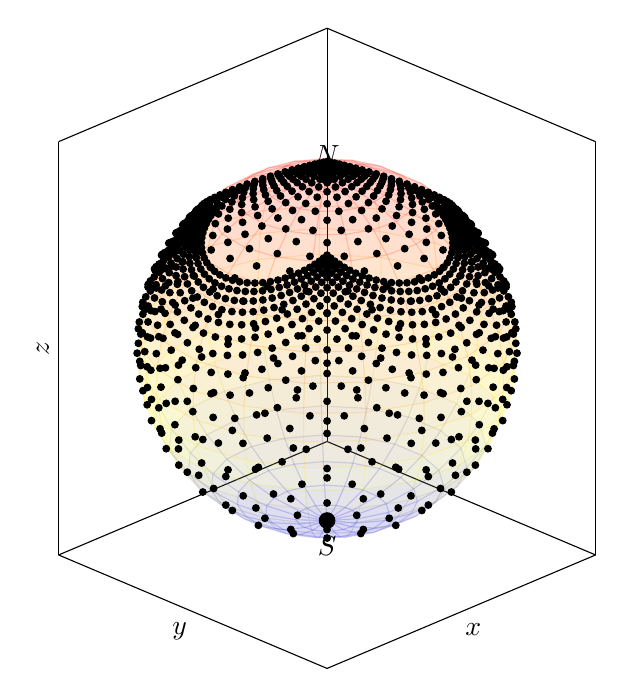
\begin{tikzpicture}
		\begin{axis}[
			view={135}{25},
			axis equal image,
			xlabel={$x$}, ylabel={$y$}, zlabel={$z$},
			ticks=none,
			% twice larger:
			width=21cm, height=15cm,
			]
			% Sphere (wireframe-ish)
			\addplot3[
			surf,
			shader=flat,
			opacity=0.10,
			domain=0:360, y domain=0:180,
			samples=20
			]
			({cos(x)*sin(y)}, {sin(x)*sin(y)}, {cos(y)});
			
			% Image of a (u,v) grid under F
			% d = 1+u^2+v^2; x=2u/d; y=-2v/d; z=(u^2+v^2-1)/d
			\addplot3[
			only marks,
			mark=*,
			mark size=1.2pt, % doubled from 0.6pt to match scale
			samples=33,
			domain=-2.2:2.2,
			y domain=-2.2:2.2
			] (
			{ 2*x/(1+x^2+y^2) },
			{ -2*y/(1+x^2+y^2) },
			{ (x^2+y^2-1)/(1+x^2+y^2) }
			);
			
			% Mark north/south poles
			\addplot3[
			only marks,
			mark=*,
			mark size=2.8pt % doubled from 1.4pt
			] coordinates {(0,0,1) (0,0,-1)};
			
			\node at (axis cs:0,0,1.12) {$N$};
			\node at (axis cs:0,0,-1.15) {$S$};
			
		\end{axis}
	\end{tikzpicture}
	\caption{The map $F|_{U_0}$ (inverse stereographic coordinates) sending the $(u,v)$-plane to $S^2\setminus\{N\}$.}
\end{figure}


\begin{figure}[H]
	\centering
	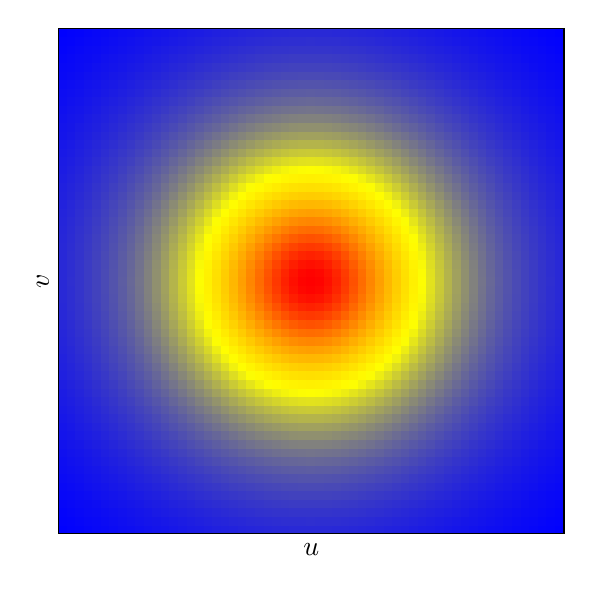
\begin{tikzpicture}
		\begin{axis}[
			axis equal image,
			xlabel={$u$}, ylabel={$v$},
			width=9.5cm, height=8cm,
			ticks=none,
			view={0}{90},
			]
			\addplot3[
			surf,
			shader=flat,
			domain=-3:3,
			y domain=-3:3,
			samples=60,
			samples y=60,
			]
			{ 2/(1 + x^2 + y^2) };
		\end{axis}
	\end{tikzpicture}
	\caption{Conformal scaling factor $\lambda(u,v)=\frac{2}{1+u^2+v^2}$ for stereographic coordinates (large near the origin, small far away).}
\end{figure}


\begin{figure}[H]
	\centering
	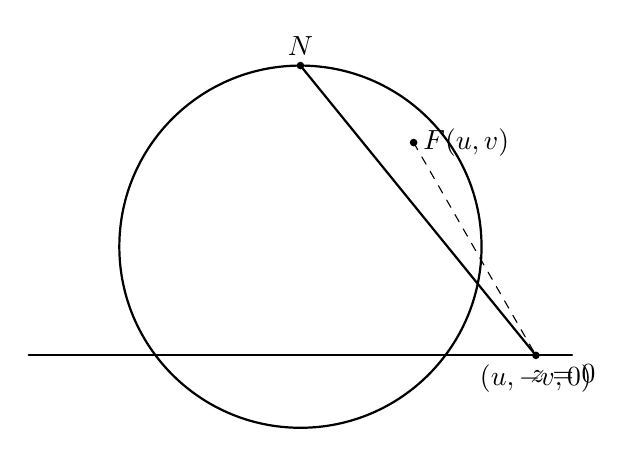
\begin{tikzpicture}[scale=1.15, line cap=round, line join=round]
		% Sphere outline (as a circle)
		\draw[thick] (0,0) circle (2);
		
		% Equatorial plane (as a line)
		\draw[thick] (-3,-1.2) -- (3,-1.2);
		\node[below] at (2.9,-1.2) {$z=0$};
		
		% North pole and a point on the plane
		\fill (0,2) circle (1.2pt);
		\node[above] at (0,2) {$N$};
		
		\fill (2.6,-1.2) circle (1.2pt);
		\node[below] at (2.6,-1.2) {$(u,-v,0)$};
		
		% A point on the sphere (image point)
		\fill (1.25,1.15) circle (1.2pt);
		\node[right] at (1.25,1.15) {$F(u,v)$};
		
		% Projection line from N
		\draw[thick] (0,2) -- (2.6,-1.2);
		
		% Indicate that the line meets the sphere
		\draw[dashed] (1.25,1.15) -- (2.6,-1.2);
	\end{tikzpicture}
	\caption{Stereographic picture: the line through $N$ and the plane point $(u,-v,0)$ meets $S^2$ at $F(u,v)$.}
\end{figure}


% ============================================================
% Problem 8
% ============================================================
\subsection*{Problem 8: The Möbius line bundle and the tautological bundle on $\mathbb{RP}^1$}

\noindent Define the Möbius bundle $M\to S^1$ to be the real line bundle trivialised over
\[
U_\pm \;=\; S^1\setminus\{(0,\pm 1)\},
\]
with transition function
\[
g_{+-}:\; U_+\cap U_- \;=\; S^1\setminus\{(0,\pm 1)\}\longrightarrow GL(1,\mathbb{R})=\mathbb{R}^\times
\]
given by $+1$ on the left-hand semicircle and $-1$ on the right-hand semicircle.
\begin{enumerate}
	\item[(a)] Show that $\mathbb{RP}^1$ is diffeomorphic to $S^1$.
	\item[(b)] Using this diffeomorphism to identify $\mathbb{RP}^1\cong S^1$, show that
	$M$ is isomorphic to the tautological bundle $\mathcal{O}_{\mathbb{RP}^1}(-1)$.
\end{enumerate}



\paragraph{\textbf{Solution.}}

\paragraph{(a) $\mathbb{RP}^1$ is diffeomorphic to $S^1$.}
Write a point of $\mathbb{RP}^1$ as $[x:y]$ with $(x,y)\neq (0,0)$ and $[x:y]=[\lambda x:\lambda y]$
for $\lambda\neq 0$.
Define
\[
\Phi:\mathbb{RP}^1 \longrightarrow S^1\subset\mathbb{R}^2,\qquad
\Phi([x:y])=\left(\frac{x^2-y^2}{x^2+y^2},\,\frac{2xy}{x^2+y^2}\right).
\]
This is well-defined since the expression is homogeneous of degree $0$ in $(x,y)$.
Moreover,
\[
\left(\frac{x^2-y^2}{x^2+y^2}\right)^2+\left(\frac{2xy}{x^2+y^2}\right)^2
=\frac{(x^2+y^2)^2}{(x^2+y^2)^2}=1,
\]
so $\Phi([x:y])\in S^1$. If $(x,y)=(\cos\theta,\sin\theta)$ then
\[
\Phi([\cos\theta:\sin\theta])=(\cos 2\theta,\sin 2\theta),
\]
so $\Phi$ is the angle-doubling map, which is precisely invariant under $\theta\sim\theta+\pi$.

To write a smooth inverse, use two charts on $S^1$:
on $S^1\setminus\{(-1,0)\}$ (where $1+X\neq 0$) set
\[
\Psi_0(X,Y)=\left[\,1:\frac{Y}{1+X}\right],
\]
and on $S^1\setminus\{(1,0)\}$ (where $1-X\neq 0$) set
\[
\Psi_1(X,Y)=\left[\,\frac{Y}{1-X}:1\right].
\]
These definitions agree on the overlap and glue to a smooth inverse $\Psi:S^1\to \mathbb{RP}^1$.
Hence $\Phi$ is a diffeomorphism $\mathbb{RP}^1\cong S^1$.

\paragraph{(b) $M \cong \mathcal{O}_{\mathbb{RP}^1}(-1)$.}
Let $\gamma^1=\mathcal{O}_{\mathbb{RP}^1}(-1)$ be the tautological real line bundle
\[
\gamma^1=\{(\ell,v)\in\mathbb{RP}^1\times\mathbb{R}^2:\ v\in \ell\}\longrightarrow \mathbb{RP}^1.
\]
Transport $\gamma^1$ to a line bundle over $S^1$ via the diffeomorphism $\Phi$, i.e.\ consider
$\widetilde{\gamma}:=(\Phi^{-1})^*(\gamma^1)\to S^1$.

Real line bundles over $S^1$ are classified by $H^1(S^1;\mathbb{Z}_2)\cong \mathbb{Z}_2$:
there are exactly two isomorphism classes, the trivial line bundle and the unique nontrivial one (the Möbius bundle).
The tautological bundle $\gamma^1$ over $\mathbb{RP}^1$ is nontrivial (equivalently $w_1(\gamma^1)\neq 0$),
hence $\widetilde{\gamma}$ is a nontrivial real line bundle over $S^1$.
Therefore $\widetilde{\gamma}$ is isomorphic to the Möbius bundle $M$ determined by the transition
function $g_{+-}$, and thus (under $\mathbb{RP}^1\cong S^1$) one has
\[
M \;\cong\; \mathcal{O}_{\mathbb{RP}^1}(-1).
\]


% ============================================================
% THEORY: Problems 8--10
% ============================================================

% ------------------------------------------------------------
% Theory for Problem 8
% ------------------------------------------------------------
\subsection*{Theory for Problem 8: Möbius line bundle, $\mathbb{RP}^1 \cong S^1$, and $\mathcal{O}_{\mathbb{RP}^1}(-1)$}

\paragraph{(8.1) Real line bundles via transition functions.}
A real line bundle $L\to X$ can be described by an open cover $\{U_i\}$ of $X$, local trivialisations
$L|_{U_i}\cong U_i\times \mathbb{R}$, and \emph{transition functions}
\[
g_{ij}:U_i\cap U_j \longrightarrow GL(1,\mathbb{R})=\mathbb{R}^\times
\]
satisfying $g_{ii}=1$ and the cocycle condition $g_{ij}\,g_{jk}=g_{ik}$ on triple overlaps.
Changing trivialisations multiplies $g_{ij}$ by a coboundary, so isomorphism classes of real line bundles
are governed by $H^1(X;\mathbb{Z}_2)$, via the first Stiefel--Whitney class $w_1(L)$.
Indeed, $\mathbb{R}^\times$ deformation retracts to $\{\pm 1\}$, so only the sign matters up to homotopy.

For $S^1$ one has
\[
H^1(S^1;\mathbb{Z}_2)\cong \mathbb{Z}_2,
\]
so there are exactly two real line bundles over $S^1$ up to isomorphism: the trivial bundle and the
nontrivial (Möbius) bundle, distinguished by $w_1=0$ versus $w_1\neq 0$.

\paragraph{(8.2) $\mathbb{RP}^1$ is a circle.}
Recall $\mathbb{RP}^1$ is the space of lines through the origin in $\mathbb{R}^2$:
\[
\mathbb{RP}^1 \;=\; \bigl(\mathbb{R}^2\setminus\{0\}\bigr)/\sim,\qquad v\sim \lambda v\ (\lambda\neq 0).
\]
Equivalently, a line is determined by a unit vector $u\in S^1$ up to the identification $u\sim -u$, hence
\[
\mathbb{RP}^1 \cong S^1/\{\pm 1\}.
\]
Topologically this quotient is again a circle. Concretely, if $\theta$ is an angle coordinate on $S^1$,
then the projective identification corresponds to $\theta\sim \theta+\pi$, and the map
\[
[\theta]\in \mathbb{R}/(\pi\mathbb{Z}) \longmapsto e^{2i\theta}\in S^1
\]
is a smooth diffeomorphism $\mathbb{RP}^1\to S^1$.

\paragraph{(8.3) The tautological bundle $\mathcal{O}_{\mathbb{RP}^1}(-1)$.}
The tautological (universal) real line bundle over $\mathbb{RP}^1$ is
\[
\gamma^1 \;=\; \mathcal{O}_{\mathbb{RP}^1}(-1)
\;=\; \{(\ell,v)\in \mathbb{RP}^1\times \mathbb{R}^2:\ v\in \ell\}\longrightarrow \mathbb{RP}^1,
\]
whose fibre over a line $\ell$ is precisely the line $\ell\subset \mathbb{R}^2$.
This bundle is nontrivial: it represents the nonzero class in $H^1(\mathbb{RP}^1;\mathbb{Z}_2)$
(equivalently $w_1(\gamma^1)\neq 0$). Since $\mathbb{RP}^1\cong S^1$ and there is a unique nontrivial
real line bundle over $S^1$, it follows that under the identification $\mathbb{RP}^1\cong S^1$,
the tautological bundle $\mathcal{O}_{\mathbb{RP}^1}(-1)$ is isomorphic to the Möbius bundle.


% ============================================================
% Problem 9
% ============================================================
\subsection*{Problem 9: Transition functions of $TS^2$ and identification with $\mathcal{O}_{\mathbb{CP}^1}(2)$}

\noindent Using the two standard stereographic projection charts, trivialise $TS^2$ over
\[
U_\pm \;=\; S^2\setminus\{(0,0,\pm 1)\},
\]
and calculate the transition function
\[
g_{+-}:\; U_+\cap U_- \longrightarrow GL(2,\mathbb{R}).
\]
Deduce that, as rank-$2$ real vector bundles,
\[
TS^2 \;\cong\; \mathcal{O}_{\mathbb{CP}^1}(2),
\]
i.e.\ viewing the fibres of $\mathcal{O}_{\mathbb{CP}^1}(2)$ as $\mathbb{R}^2$ instead of $\mathbb{C}$.



\paragraph{\textbf{Solution.}}
Let $N=(0,0,1)$ and $S=(0,0,-1)$, and set
\[
U_+ = S^2\setminus\{N\},\qquad U_- = S^2\setminus\{S\}.
\]
Let $\phi_\pm:U_\pm\to \mathbb{R}^2\cong\mathbb{C}$ be the stereographic charts.
Using $\phi_\pm$, trivialise the tangent bundle by
\[
TS^2|_{U_\pm}\;\cong\; U_\pm\times \mathbb{R}^2,\qquad
v\in T_pS^2\longmapsto d(\phi_\pm)_p(v)\in \mathbb{R}^2.
\]
On the overlap $U_+\cap U_-$, the transition function is the Jacobian of the coordinate change:
\[
g_{+-}(p)=d\bigl(\phi_-\circ \phi_+^{-1}\bigr)\Big|_{\phi_+(p)}\in GL(2,\mathbb{R}).
\]

\paragraph{(1) Computing $g_{+-}$.}
With the standard stereographic conventions (and possibly composing one chart with complex conjugation),
the overlap map on $\mathbb{C}^\times$ can be written as
\[
w=\phi_-\circ\phi_+^{-1}(z)=\frac{1}{z},\qquad z\in\mathbb{C}^\times.
\]
Write $z=u+iv$ and $w=u'+iv'$. Then
\[
w=\frac{1}{u+iv}=\frac{u-iv}{u^2+v^2}
\quad\Longrightarrow\quad
(u',v')=\left(\frac{u}{u^2+v^2},\,-\frac{v}{u^2+v^2}\right).
\]
Let $\rho^2=u^2+v^2$. Differentiating gives
\[
D(u',v')
=
\frac{1}{\rho^4}
\begin{pmatrix}
	v^2-u^2 & -2uv\\
	2uv & v^2-u^2
\end{pmatrix}.
\]
Hence, in the chosen trivialisations,
\[
\boxed{
	g_{+-}(u,v)=
	\frac{1}{(u^2+v^2)^2}
	\begin{pmatrix}
		v^2-u^2 & -2uv\\
		2uv & v^2-u^2
	\end{pmatrix}
	\in GL(2,\mathbb{R}),\qquad (u,v)\neq(0,0).
}
\]
Equivalently, in complex notation, since $w=1/z$ one has
\[
dw=\left(-\frac{1}{z^2}\right)dz,
\]
so $g_{+-}$ is the real $2\times 2$ matrix representing multiplication by $-1/z^2$ on $\mathbb{C}\cong\mathbb{R}^2$
(the constant $-1$ can be absorbed by changing the frame on one chart).

\paragraph{(2) Deduce $TS^2\cong \mathcal{O}_{\mathbb{CP}^1}(2)$ as real rank-$2$ bundles.}
Under the identification $S^2\cong\mathbb{CP}^1$ (Riemann sphere), take affine coordinates
$z$ on $U_0=\{[1:z]\}$ and $w=1/z$ on $U_1=\{[w:1]\}$. Then the holomorphic tangent frames satisfy
\[
\frac{\partial}{\partial z}
=
\frac{dw}{dz}\frac{\partial}{\partial w}
=
\left(-\frac{1}{z^2}\right)\frac{\partial}{\partial w}.
\]
Thus the transition function of $T\mathbb{CP}^1$ is $-z^{-2}$, which agrees with that of $\mathcal{O}_{\mathbb{CP}^1}(2)$
up to the constant factor $-1$ (a gauge change). Therefore, as complex line bundles,
\[
T\mathbb{CP}^1 \cong \mathcal{O}_{\mathbb{CP}^1}(2).
\]
Viewing a complex line bundle as a real rank-$2$ bundle via $\mathbb{C}\cong\mathbb{R}^2$ yields
\[
TS^2 \;\cong\; \bigl(T\mathbb{CP}^1\bigr)_{\mathbb{R}}
\;\cong\; \bigl(\mathcal{O}_{\mathbb{CP}^1}(2)\bigr)_{\mathbb{R}},
\]
as required.


% ------------------------------------------------------------
% Theory for Problem 9
% ------------------------------------------------------------
\subsection*{Theory for Problem 9: Transition functions of $TS^2$ and identification with $\mathcal{O}_{\mathbb{CP}^1}(2)$}

\paragraph{(9.1) Stereographic charts on $S^2$.}
Let $S^2\subset \mathbb{R}^3$, and let $N=(0,0,1)$ and $S=(0,0,-1)$ be the north and south poles.
Define the standard cover
\[
U_+ = S^2\setminus\{N\},\qquad U_- = S^2\setminus\{S\}.
\]
Stereographic projection gives diffeomorphisms
\[
\phi_+:U_+\to \mathbb{R}^2 \cong \mathbb{C},\qquad
\phi_-:U_-\to \mathbb{R}^2 \cong \mathbb{C}.
\]
On the overlap $U_+\cap U_- = S^2\setminus\{N,S\}$, the coordinate change
\[
\phi_- \circ \phi_+^{-1}:\ \mathbb{C}^\times \longrightarrow \mathbb{C}^\times
\]
is (up to a convention) the inversion map
\[
w = \frac{1}{z}.
\]
This map is conformal; its complex derivative is $dw/dz = -1/z^2$.

\paragraph{(9.2) Tangent bundle transition functions from Jacobians.}
Given a chart $\phi:U\to \mathbb{R}^2$, a standard trivialisation of the tangent bundle over $U$ is
\[
TS^2|_U \cong U\times \mathbb{R}^2,\qquad
v\in T_pS^2 \mapsto (p,\, d\phi_p(v))\in U\times \mathbb{R}^2.
\]
Hence, on an overlap $U_+\cap U_-$ the transition function for $TS^2$ is given by the Jacobian matrix:
\[
g_{+-}(p)\;=\; d(\phi_- \circ \phi_+^{-1})\big|_{\phi_+(p)} \in GL(2,\mathbb{R}).
\]
Thus computing $g_{+-}$ reduces to differentiating the overlap map in local coordinates.

\paragraph{(9.3) Why $\mathcal{O}_{\mathbb{CP}^1}(2)$ appears.}
Using the identification $\mathbb{CP}^1\cong S^2$ (the Riemann sphere), one has the classical
holomorphic line bundle isomorphism
\[
T\mathbb{CP}^1 \cong \mathcal{O}_{\mathbb{CP}^1}(2).
\]
One way to see this is via the Euler sequence on $\mathbb{CP}^1$, or by the degree computation
$c_1(T\mathbb{CP}^1)=2$.
If we forget the complex structure, a complex line bundle becomes a real rank-$2$ vector bundle.
Thus, viewing fibres of $\mathcal{O}_{\mathbb{CP}^1}(2)$ as $\mathbb{R}^2$ rather than $\mathbb{C}$,
the statement $TS^2 \cong \mathcal{O}_{\mathbb{CP}^1}(2)$ is an identification of real rank-$2$ bundles.
At the level of transition functions: if $w=1/z$ on overlaps, then tangent vectors transform by
\[
\frac{\partial}{\partial z} = \frac{dw}{dz}\,\frac{\partial}{\partial w},\qquad \frac{dw}{dz}=-\frac{1}{z^2},
\]
which is precisely the $z^{-2}$ (degree $2$) behaviour encoded by $\mathcal{O}(2)$.


% ============================================================
% Problem 10
% ============================================================
\subsection*{Problem 10: Derivations at a point and the tangent space}

\noindent Fix a smooth manifold $X$ and a point $p\in X$. Let $\mathcal{O}_{X,p}$ be the space of germs
of smooth functions about $p$; this is an $\mathbb{R}$-vector space by scalar multiplication.
An $\mathbb{R}$-linear derivation $\mathcal{O}_{X,p}\to\mathbb{R}$ is an $\mathbb{R}$-linear map $d$ such that
\[
d(fg)\;=\; d(f)\,g(p) + f(p)\,d(g)
\qquad\text{for all germs } f,g.
\]
These form an $\mathbb{R}$-vector space denoted $\mathrm{Der}_{\mathbb{R}}(\mathcal{O}_{X,p},\mathbb{R})$.
Show that this vector space is naturally isomorphic to the tangent space $T_pX$.




\paragraph{\textbf{Solution.}}
Let $X$ be a smooth manifold and $p\in X$. Let $\mathcal{O}_{X,p}$ denote the $\mathbb{R}$-algebra of germs
of smooth functions at $p$. An $\mathbb{R}$-linear derivation is an $\mathbb{R}$-linear map
$d:\mathcal{O}_{X,p}\to \mathbb{R}$ such that
\[
d(fg)=d(f)\,g(p)+f(p)\,d(g).
\]
We construct a natural isomorphism
\[
\mathrm{Der}_{\mathbb{R}}(\mathcal{O}_{X,p},\mathbb{R}) \cong T_pX.
\]

\paragraph{Step 1: $T_pX \to \mathrm{Der}_{\mathbb{R}}(\mathcal{O}_{X,p},\mathbb{R})$.}
Given $v\in T_pX$, define $d_v:\mathcal{O}_{X,p}\to \mathbb{R}$ by
\[
d_v([f]) := (df)_p(v).
\]
This is well-defined on germs, $\mathbb{R}$-linear, and satisfies the Leibniz rule since
\[
d_v(fg) = v(fg) = v(f)\,g(p) + f(p)\,v(g).
\]
Thus we obtain a linear map
\[
\Phi:T_pX\to \mathrm{Der}_{\mathbb{R}}(\mathcal{O}_{X,p},\mathbb{R}),\qquad \Phi(v)=d_v.
\]

\paragraph{Step 2: Derivations kill $\mathfrak{m}_p^2$.}
Let $\mathfrak{m}_p=\{f\in \mathcal{O}_{X,p}: f(p)=0\}$ be the maximal ideal.
If $g,h\in \mathfrak{m}_p$, then $g(p)=h(p)=0$, so by Leibniz
\[
d(gh)=d(g)\,h(p)+g(p)\,d(h)=0.
\]
Hence every derivation vanishes on $\mathfrak{m}_p^2$.

\paragraph{Step 3: Local coordinate description.}
Choose a chart $(U,x^1,\dots,x^n)$ around $p$, and assume (after translation) that $x^i(p)=0$.
Given $d\in \mathrm{Der}_{\mathbb{R}}(\mathcal{O}_{X,p},\mathbb{R})$, set
\[
a^i := d(x^i)\in \mathbb{R}.
\]
For any $f\in\mathcal{O}_{X,p}$, write a first-order Taylor expansion in coordinates:
\[
f(x)=f(p)+\sum_{i=1}^n \frac{\partial f}{\partial x^i}(p)\,x^i + \sum_{i,j} x^i x^j\,h_{ij}(x),
\]
where the $h_{ij}$ are smooth. The remainder term lies in $\mathfrak{m}_p^2$, hence is killed by $d$.
Therefore,
\[
d(f)= d\!\left(\sum_{i=1}^n \frac{\partial f}{\partial x^i}(p)\,x^i\right)
=\sum_{i=1}^n \frac{\partial f}{\partial x^i}(p)\,d(x^i)
=\sum_{i=1}^n a^i\,\frac{\partial f}{\partial x^i}(p).
\]

\paragraph{Step 4: Construct the inverse and conclude.}
Define
\[
v_d := \sum_{i=1}^n a^i\,\frac{\partial}{\partial x^i}\Big|_p \in T_pX.
\]
Then for all $f$,
\[
(df)_p(v_d)=\sum_{i=1}^n a^i\,\frac{\partial f}{\partial x^i}(p)=d(f),
\]
so $d=\Phi(v_d)$. Hence $\Phi$ is surjective. If $\Phi(v)=0$, then $v(x^i)=0$ for all $i$,
so $v=0$, hence $\Phi$ is injective. Therefore $\Phi$ is an isomorphism.

Finally, the map $v\mapsto (f\mapsto (df)_p(v))$ is intrinsic and does not depend on the choice of chart,
so the isomorphism is natural. Consequently,
\[
\mathrm{Der}_{\mathbb{R}}(\mathcal{O}_{X,p},\mathbb{R}) \cong T_pX.
\]


% ------------------------------------------------------------
% Theory for Problem 10
% ------------------------------------------------------------
\subsection*{Theory for Problem 10: Derivations of germs and the tangent space}

\paragraph{(10.1) Germs and the maximal ideal.}
Let $\mathcal{O}_{X,p}$ be the $\mathbb{R}$-algebra of germs of smooth functions at $p$.
There is an evaluation map
\[
\mathrm{ev}_p:\mathcal{O}_{X,p}\to \mathbb{R},\qquad [f]\mapsto f(p).
\]
Its kernel is the maximal ideal
\[
\mathfrak{m}_p \;=\; \{\,f\in \mathcal{O}_{X,p}:\ f(p)=0\,\}.
\]

\paragraph{(10.2) Derivations and the Leibniz rule.}
An $\mathbb{R}$-linear derivation is an $\mathbb{R}$-linear map $d:\mathcal{O}_{X,p}\to \mathbb{R}$ such that
\[
d(fg)=d(f)\,g(p)+f(p)\,d(g)
\]
for all germs $f,g$. Immediate consequences include $d(1)=0$. Moreover, if $f,g\in \mathfrak{m}_p$ then
$f(p)=g(p)=0$ and hence $d(fg)=0$. Thus every derivation kills $\mathfrak{m}_p^2$, and therefore factors as
\[
\mathfrak{m}_p \twoheadrightarrow \mathfrak{m}_p/\mathfrak{m}_p^2 \xrightarrow{\;\;\bar d\;\;} \mathbb{R}.
\]
In particular,
\[
\mathrm{Der}_{\mathbb{R}}(\mathcal{O}_{X,p},\mathbb{R})
\;\cong\;
\mathrm{Hom}_{\mathbb{R}}\bigl(\mathfrak{m}_p/\mathfrak{m}_p^2,\mathbb{R}\bigr).
\]
The quotient $\mathfrak{m}_p/\mathfrak{m}_p^2$ is the (algebraic) cotangent space $T_p^*X$,
and its dual is the tangent space $T_pX$.

\paragraph{(10.3) Tangent vectors as directional derivatives.}
A tangent vector $v\in T_pX$ defines a derivation by directional differentiation:
\[
d_v([f]) \;:=\; v(f) \;=\; \left.\frac{d}{dt}\right|_{t=0} (f\circ \gamma)(t),
\]
where $\gamma$ is any smooth curve with $\gamma(0)=p$ and $\gamma'(0)=v$.
This satisfies the Leibniz rule, hence gives a map
\[
T_pX \longrightarrow \mathrm{Der}_{\mathbb{R}}(\mathcal{O}_{X,p},\mathbb{R}),\qquad v\mapsto d_v.
\]
Conversely, in local coordinates $(x^1,\dots,x^n)$ near $p$, any derivation $d$ is determined by the scalars
$a^i:=d(x^i)$, since $d$ depends only on the first-order Taylor part (it vanishes on $\mathfrak{m}_p^2$).
Thus, in coordinates,
\[
d \;=\; \sum_{i=1}^n a^i \frac{\partial}{\partial x^i}\Big|_p,
\]
which identifies derivations with tangent vectors and yields the natural isomorphism
\[
\mathrm{Der}_{\mathbb{R}}(\mathcal{O}_{X,p},\mathbb{R}) \;\cong\; T_pX.
\]
	
	
	
	% ============================================================
	% Problem 1
	% ============================================================
	\subsection*{Problem 1: Canonical tensor--Hom identification and contraction as composition}
	
	\noindent Let $T,U,V$ be finite-dimensional vector spaces over a field $\Bbb K$.
	Let $e_1,\dots,e_m$ be a basis of $U$ with dual basis $\varepsilon^1,\dots,\varepsilon^m$,
	and let $f_1,\dots,f_n$ be a basis of $V$.
	\begin{enumerate}
		\item[(a)] Show that there is a canonical isomorphism $V\otimes U^\vee \cong \mathcal L(U,V)$.
		\item[(b)] Given $\alpha\in \mathcal L(U,V)$, viewed as an element of $V\otimes U^\vee$,
		what is the meaning of its components with respect to the basis $f_i\otimes \varepsilon^j$?
		\item[(c)] Show that contraction
		\[
		V\otimes U^\vee\otimes U\otimes T^\vee \longrightarrow V\otimes T^\vee
		\]
		corresponds to the composition map
		\[
		\mathcal L(U,V)\otimes \mathcal L(T,U)\longrightarrow \mathcal L(T,V).
		\]
	\end{enumerate}
	
	
	\subsection*{Theory for Problem 1: $V\otimes U^\vee \cong \mathcal L(U,V)$ and contraction = composition}
	
	\paragraph{\textbf{Dual space and evaluation.}}
	For a finite-dimensional $\Bbb K$-vector space $U$, its dual is
	\[
	U^\vee=\mathrm{Hom}_\Bbb K(U,\Bbb K).
	\]
	There is a canonical bilinear pairing (evaluation)
	\[
	\langle \varphi,u\rangle := \varphi(u),\qquad U^\vee\times U\to \Bbb K.
	\]
	Given a basis $(e_j)$ of $U$, the dual basis $(\varepsilon^j)\subset U^\vee$ is characterised by
	\[
	\varepsilon^j(e_k)=\delta^j_k.
	\]
	
	\paragraph{\textbf{Canonical tensor--Hom isomorphism.}}
	Define a map
	\[
	\Theta: V\otimes U^\vee \longrightarrow \mathcal L(U,V)
	\]
	on pure tensors by
	\[
	\Theta(v\otimes \varphi)(u) := \varphi(u)\,v,\qquad v\in V,\ \varphi\in U^\vee,\ u\in U,
	\]
	and extend linearly. This uses only evaluation, hence is canonical (basis-free). In finite dimensions,
	$\Theta$ is an isomorphism (e.g.\ by a dimension count and checking it is injective/surjective).
	
	\paragraph{\textbf{Components and matrix entries.}}
	Fix bases $e_1,\dots,e_m$ of $U$ with dual basis $\varepsilon^1,\dots,\varepsilon^m$ and
	$f_1,\dots,f_n$ of $V$. For $\alpha\in\mathcal L(U,V)$ write
	\[
	\alpha(e_j)=\sum_{i=1}^n a_{ij} f_i.
	\]
	Then under $\Theta^{-1}:\mathcal L(U,V)\to V\otimes U^\vee$, the map $\alpha$ corresponds to
	\[
	\sum_{i=1}^n\sum_{j=1}^m a_{ij}\, f_i\otimes \varepsilon^j.
	\]
	Thus the coefficients $a_{ij}$ are simultaneously the matrix entries of $\alpha$ and the components
	of the associated tensor in the basis $f_i\otimes \varepsilon^j$.
	
	\paragraph{\textbf{Contraction as composition.}}
	The pairing $U^\vee\otimes U\to \Bbb K$ induces the contraction map
	\[
	\mathrm{contr}:\; V\otimes U^\vee\otimes U\otimes T^\vee \longrightarrow V\otimes T^\vee,
	\]
	defined on pure tensors by
	\[
	\mathrm{contr}(v\otimes \varphi \otimes u\otimes \psi)
	:= \varphi(u)\,(v\otimes \psi).
	\]
	Using the identifications
	\[
	V\otimes U^\vee \cong \mathcal L(U,V),
	\qquad
	U\otimes T^\vee \cong \mathcal L(T,U),
	\]
	one checks on pure tensors that contraction corresponds exactly to composition:
	if $A=\Theta(v\otimes\varphi)$ and $B=\Theta(u\otimes\psi)$, then
	\[
	(A\circ B)(t) = \psi(t)\,\varphi(u)\,v,
	\]
	which corresponds to $\varphi(u)\,v\otimes \psi = \mathrm{contr}(v\otimes\varphi\otimes u\otimes\psi)$.
	Hence $\mathrm{contr}$ matches the composition map
	\[
	\mathcal L(U,V)\otimes \mathcal L(T,U)\longrightarrow \mathcal L(T,V).
	\]
	
	
	% ============================================================
	% Problem 2
	% ============================================================
	\subsection*{Problem 2: Triviality of $M\oplus M$ and stable triviality of $TS^n$}
	
	\begin{enumerate}
		\item[(a)] Recall the Möbius bundle $M\to S^1$ from Sheet~1. Show that $M\oplus M$ is trivial.
		\item[(b)] Show that for all $n$ we have
		\[
		TS^n \oplus \mathbb{R} \;\cong\; \mathbb{R}^{n+1}
		\]
		as vector bundles over $S^n$.
		\emph{Hint:} View $\mathbb{R}^{n+1}$ as $\iota^*T\mathbb{R}^{n+1}$, where $\iota:S^n\hookrightarrow \mathbb{R}^{n+1}$
		is the inclusion.
	\end{enumerate}
	
	
	% ============================================================
	% Theory for Problem 2
	% ============================================================
	\subsection*{Theory for Problem 2: $M\oplus M$ and stable triviality of $TS^n$}
	
	\paragraph{\textbf{(2a) Why $M\oplus M$ is trivial.}}
	The Möbius bundle $M\to S^1$ is the unique nontrivial real line bundle over the circle.
	Using transition functions on a two-set cover, $M$ has transition $g_{+-}:U_+\cap U_-\to \{\pm 1\}\subset GL(1,\mathbb R)$
	which (up to convention) equals $-1$ on one connected component of the overlap.
	For a direct sum, transition functions become block diagonal:
	\[
	g^{M\oplus M}_{+-}=
	\begin{pmatrix}
		g_{+-} & 0\\
		0 & g_{+-}
	\end{pmatrix}.
	\]
	Thus on the nontrivial component one has $g^{M\oplus M}_{+-}=-I_2\in GL(2,\mathbb R)$.
	But $-I_2$ is homotopic to $I_2$ inside $GL(2,\mathbb R)$ (e.g.\ through rotations in $SO(2)$),
	so after a change of local frames the transition becomes $I_2$, i.e.\ $M\oplus M$ is trivial.
	
	Equivalently, using Stiefel--Whitney classes, line bundles over $S^1$ are classified by
	$w_1\in H^1(S^1;\mathbb Z_2)\cong \mathbb Z_2$, and
	\[
	w_1(M\oplus M)=w_1(M)+w_1(M)=0,
	\]
	so the rank-$2$ bundle $M\oplus M$ is orientable; over $S^1$ this implies triviality.
	
	\paragraph{\textbf{(2b) Stable triviality of the tangent bundle of $S^n$.}}
	Let $\iota:S^n\hookrightarrow \mathbb R^{n+1}$ be the inclusion. Since $T\mathbb R^{n+1}$ is trivial,
	its pullback is trivial:
	\[
	\iota^*T\mathbb R^{n+1}\cong S^n\times \mathbb R^{n+1}.
	\]
	At each $p\in S^n$, the tangent space splits orthogonally as
	\[
	T_p\mathbb R^{n+1} = T_pS^n \oplus \langle p\rangle,
	\]
	where $\langle p\rangle$ is the normal line spanned by the radius vector $p$.
	The normal line bundle is therefore trivial, with global nowhere-zero normal section $p\mapsto p$:
	\[
	\nu \cong S^n\times \mathbb R.
	\]
	Hence, as vector bundles over $S^n$,
	\[
	\iota^*T\mathbb R^{n+1} \cong TS^n \oplus \nu \cong TS^n \oplus \mathbb R.
	\]
	Combining with $\iota^*T\mathbb R^{n+1}\cong S^n\times \mathbb R^{n+1}$ yields
	\[
	TS^n\oplus \mathbb R \cong \mathbb R^{n+1}.
	\]


% ============================================================
% Fiber bundles: definition (and vector bundles / line bundles)
% ============================================================

\subsection*{Fiber bundles and real line bundles (definitions)}

\paragraph{Fiber bundle: definition.}
Let $E,B,F$ be topological spaces. A \emph{fiber bundle} with \emph{total space} $E$,
\emph{base space} $B$, \emph{fiber} $F$, and \emph{projection} $\pi:E\to B$ is a continuous
surjective map
\[
\pi:E\longrightarrow B
\]
together with the following \emph{local triviality} property:

There exists an open cover $\{U_i\}_{i\in I}$ of $B$ and homeomorphisms (called
\emph{local trivializations})
\[
\Phi_i:\pi^{-1}(U_i)\longrightarrow U_i\times F
\]
such that
\[
\pi \;=\; \mathrm{pr}_1\circ \Phi_i\quad\text{on }\pi^{-1}(U_i),
\]
where $\mathrm{pr}_1:U_i\times F\to U_i$ is the projection to the first factor.

Equivalently, for each $b\in U_i$, the restriction
\[
\Phi_i\big|_{\pi^{-1}(b)}:\pi^{-1}(b)\longrightarrow \{b\}\times F \cong F
\]
is a homeomorphism, so every fiber $\pi^{-1}(b)$ is (locally, in families) homeomorphic
to $F$.

\paragraph{Trivial bundle.}
A fiber bundle is \emph{trivial} if it is globally isomorphic to a product:
\[
E\cong B\times F,\qquad \pi=\mathrm{pr}_1.
\]

\paragraph{Bundle maps and bundle isomorphisms.}
Given two fiber bundles $\pi:E\to B$ and $\pi':E'\to B$ over the same base $B$ (with the
same fiber type), a \emph{bundle map} covering the identity is a continuous map
\[
\Psi:E\to E'
\]
such that
\[
\pi' \circ \Psi = \pi.
\]
It is a \emph{bundle isomorphism} if, in addition, $\Psi$ is a homeomorphism and restricts
to a homeomorphism on each fiber.

\paragraph{Transition functions (how bundles glue).}
Given trivializations $\Phi_i$ and $\Phi_j$ on $U_i$ and $U_j$, the \emph{change of
	trivialization} on overlaps $U_i\cap U_j$ is the homeomorphism
\[
\Phi_i\circ \Phi_j^{-1}:(U_i\cap U_j)\times F \longrightarrow (U_i\cap U_j)\times F.
\]
Because it preserves the base point, it has the form
\[
\Phi_i\circ \Phi_j^{-1}(b,f)=(b,\,g_{ij}(b)(f)),
\]
where
\[
g_{ij}:U_i\cap U_j\to \mathrm{Homeo}(F)
\]
is called the \emph{transition function}. The transition functions satisfy cocycle
identities on triple overlaps:
\[
g_{ii}=\mathrm{id},\qquad g_{ij}=g_{ji}^{-1},\qquad g_{ij}\,g_{jk}\,g_{ki}=\mathrm{id}.
\]

\paragraph{Vector bundle: definition.}
A \emph{real vector bundle of rank $n$} over $B$ is a fiber bundle $\pi:E\to B$ with fiber
$\mathbb{R}^n$ such that:
\begin{itemize}
	\item each fiber $E_b=\pi^{-1}(b)$ is endowed with a real vector space structure, and
	\item there exists an open cover $\{U_i\}$ and local trivializations
	\[
	\Phi_i:\pi^{-1}(U_i)\to U_i\times \mathbb{R}^n
	\]
	for which each fiber map
	\[
	\Phi_i\big|_{E_b}:E_b\to \{b\}\times \mathbb{R}^n\cong \mathbb{R}^n
	\]
	is a linear isomorphism.
\end{itemize}
Equivalently, the transition functions take values in the linear group:
\[
g_{ij}:U_i\cap U_j\to GL(n,\mathbb{R}),\qquad
\Phi_i\circ\Phi_j^{-1}(b,v)=(b,\,g_{ij}(b)\,v).
\]

\paragraph{Real line bundle.}
A \emph{real line bundle} is a rank-$1$ real vector bundle. Thus its fiber is
$\mathbb{R}$, and its transition functions land in
\[
GL(1,\mathbb{R})=\mathbb{R}^\times.
\]
The Möbius bundle is the unique (up to isomorphism) nontrivial real line bundle over
$S^1$.

	
% ============================================================
% Möbius bundle M -> S^1
% ============================================================

\subsection*{Möbius bundle $M\to S^1$}

\paragraph{Möbius bundle $M\to S^1$: what it is (geometric picture).}
The \emph{Möbius bundle} is the nontrivial real line bundle over the circle.
Its total space is the Möbius strip, obtained by gluing the ends of a strip
with a half-twist:
\[
M \;=\;\bigl([0,1]\times \mathbb{R}\bigr)\Big/\bigl((0,t)\sim(1,-t)\bigr)
\;\longrightarrow\;
S^1 \;=\; [0,1]/(0\sim 1),
\]
with projection induced by
\[
(s,t)\longmapsto [s]\in S^1.
\]
Going once around the base circle flips the fiber coordinate $t\mapsto -t$.
That single sign flip after one loop is exactly the ``twist''.

\paragraph{As the tautological bundle on $\mathbb{RP}^1$.}
Equivalently, $M$ is the tautological line bundle over real projective space
\[
M \;\cong\; \mathcal{O}_{\mathbb{RP}^1}(-1).
\]
A point $[\ell]\in \mathbb{RP}^1$ is a line $\ell\subset \mathbb{R}^2$, and the
fiber over $[\ell]$ is \emph{that very line}:
\[
M_{[\ell]}=\ell\subset \mathbb{R}^2.
\]
Using the identification $\mathbb{RP}^1\simeq S^1$, this tautological bundle
becomes the Möbius line bundle over $S^1$.

\paragraph{Transition-function description.}
Let $\{U_+,U_-\}$ be an open cover of $S^1$ such that
$U_+\cap U_-$ has two connected components (two arcs). A real line bundle is
determined (up to isomorphism) by a transition function
\[
g_{+-}:U_+\cap U_- \longrightarrow GL(1,\mathbb{R})=\mathbb{R}^\times.
\]
Since $\mathbb{R}^\times$ deformation retracts onto $\{\pm 1\}$, for
classification one may take $g_{+-}\in\{\pm 1\}$ on each overlap component.

\medskip
\noindent\textbf{Trivial bundle.}
If $g_{+-}\equiv +1$ on both overlap components, the gluing has no twist and
the bundle is the product:
\[
S^1\times \mathbb{R}.
\]

\medskip
\noindent\textbf{Möbius bundle.}
For the Möbius bundle one overlap component glues with $+1$ and the other with
$-1$:
\[
g_{+-}=
\begin{cases}
	+1 & \text{on one component of }U_+\cap U_-,\\
	-1 & \text{on the other component of }U_+\cap U_-.
\end{cases}
\]
Crossing the ``$-1$'' overlap flips a local frame by a sign. This pattern cannot
be removed by changing local trivializations, and it gives the unique nontrivial
class in
\[
H^1(S^1;\mathbb{Z}_2)\;\cong\;\mathbb{Z}_2.
\]

\paragraph{Basic intuition checks.}

\textbf{(1) No nowhere-zero global section.}
If $s:S^1\to M$ were a nowhere-zero section, it would pick a nonzero vector
continuously in each fiber. After one loop around $S^1$ the chosen vector must
return with opposite sign (because of the twist), which forces a zero somewhere.
Hence every continuous section of $M$ vanishes at some point.

\textbf{(2) Pullback along the double cover becomes trivial.}
Let $\pi:S^1\to S^1$ be the degree-$2$ covering map $\pi(e^{i\theta})=e^{2i\theta}$.
Then
\[
\pi^*(M)\;\cong\; S^1\times \mathbb{R}.
\]
Intuitively: going around the base twice cancels the sign flip.

\textbf{(3) Stiefel--Whitney class.}
Real line bundles over $S^1$ are classified by $w_1\in H^1(S^1;\mathbb{Z}_2)$:
\[
w_1(M)\neq 0,\qquad w_1(S^1\times \mathbb{R})=0.
\]

\paragraph{Why $M\oplus M$ is trivial (matrix / transition view).}
If $M$ has transition $g_{+-}\in\{\pm 1\}$, then the rank-$2$ bundle $M\oplus M$
has transition
\[
g_{+-}^{\,M\oplus M}=
\begin{pmatrix}
	g_{+-} & 0\\[2pt]
	0 & g_{+-}
\end{pmatrix}
\in GL(2,\mathbb{R}).
\]
On the overlap component where $g_{+-}=-1$, this is $-I_2$.

A change of local frames by $A_+:U_+\to GL(2,\mathbb{R})$ and
$A_-:U_-\to GL(2,\mathbb{R})$ changes the transition to
\[
(g_{+-})' \;=\; A_+\, g_{+-}^{\,M\oplus M}\, A_-^{-1}.
\]
The key point is that $-I_2$ is path-connected to $I_2$ inside $GL(2,\mathbb{R})$.
Indeed, inside $SO(2)\subset GL(2,\mathbb{R})$ the rotation matrices
\[
R(\theta)=
\begin{pmatrix}
	\cos\theta & -\sin\theta\\
	\sin\theta & \cos\theta
\end{pmatrix}
\]
satisfy $R(0)=I_2$ and $R(\pi)=-I_2$. Thus one can ``spread'' this rotation
through a local change of frame so that the overlap transition becomes $I_2$,
and the bundle trivializes:
\[
M\oplus M \;\cong\; S^1\times \mathbb{R}^2.
\]

\paragraph{Short obstruction argument (via $w_1$).}
For Whitney sums,
\[
w_1(M\oplus M)=w_1(M)+w_1(M)=0\in H^1(S^1;\mathbb{Z}_2).
\]
So $M\oplus M$ is orientable. Every orientable rank-$2$ real vector bundle over
$S^1$ is trivial (after fixing orientation one builds a global orthonormal
frame), hence again
\[
M\oplus M \;\cong\; S^1\times \mathbb{R}^2.
\]

	% ============================================================
	% Möbius bundle M -> S^1
	% ============================================================
	
	\subsection*{Möbius bundle $M\to S^1$}
	
	\paragraph{Real line bundle: definition (rank-$1$ real vector bundle).}
	A \emph{real line bundle} over a space $B$ is a fiber bundle
	\[
	\pi:E\to B
	\]
	such that each fiber $E_b=\pi^{-1}(b)$ is a $1$-dimensional real vector space and,
	locally on $B$, the bundle is trivial as a vector bundle: there exists an open cover
	$\{U_i\}_{i\in I}$ of $B$ and homeomorphisms
	\[
	\Phi_i:\pi^{-1}(U_i)\longrightarrow U_i\times\mathbb{R}
	\]
	satisfying:
	\begin{itemize}
		\item $\pi=\mathrm{pr}_1\circ \Phi_i$ on $\pi^{-1}(U_i)$, and
		\item for each $b\in U_i$, the restriction
		\[
		\Phi_i\big|_{E_b}:E_b\longrightarrow \{b\}\times\mathbb{R}\cong \mathbb{R}
		\]
		is a linear isomorphism of real vector spaces.
	\end{itemize}
	On overlaps $U_i\cap U_j$, the two trivializations differ by a \emph{transition function}
	\[
	g_{ij}:U_i\cap U_j\to GL(1,\mathbb{R})=\mathbb{R}^\times
	\]
	defined by
	\[
	\Phi_i\circ \Phi_j^{-1}(b,t)=(b,\,g_{ij}(b)\,t),
	\]
	and the cocycle conditions hold:
	\[
	g_{ii}=1,\qquad g_{ij}=g_{ji}^{-1},\qquad g_{ij}\,g_{jk}\,g_{ki}=1\quad\text{on }U_i\cap U_j\cap U_k.
	\]
	
	\paragraph{Möbius bundle $M\to S^1$: total space and projection.}
	The \emph{Möbius bundle} is the nontrivial real line bundle over the circle. One concrete
	model is obtained by taking the strip $[0,1]\times\mathbb{R}$ and gluing its ends with a
	sign flip in the fiber coordinate:
	\[
	M \;=\;\bigl([0,1]\times\mathbb{R}\bigr)\Big/\bigl((0,t)\sim(1,-t)\bigr).
	\]
	Let $[s,t]$ denote the equivalence class of $(s,t)$. The base is
	\[
	S^1 \;=\; [0,1]/(0\sim 1),
	\]
	and the bundle projection is induced by the map $(s,t)\mapsto [s]$:
	\[
	\pi:M\to S^1,\qquad \pi([s,t])=[s].
	\]
	The fiber over $[s]\in S^1$ is
	\[
	M_{[s]}=\{[s,t]:t\in\mathbb{R}\}\cong \mathbb{R},
	\]
	and the vector space structure on each fiber is inherited from the $\mathbb{R}$-coordinate
	$t$ (this is well-defined because the gluing map $(0,t)\sim(1,-t)$ is linear in $t$).
	
	\paragraph{Geometric picture: ``flip after one loop''.}
	Choose a point $b=[s]\in S^1$ and a nonzero vector $t\neq 0$ in the fiber $M_b$.
	If you move continuously once around the base circle and transport the same local fiber
	coordinate through the identification, when you return to the starting base point the
	fiber coordinate has changed sign:
	\[
	t \longmapsto -t.
	\]
	This ``sign flip after one circuit'' is the half-twist that distinguishes the Möbius
	bundle from the trivial product bundle $S^1\times\mathbb{R}$.
	
	\paragraph{Local trivializations (charts) on $S^1$ and explicit transition.}
	Write $S^1=[0,1]/(0\sim 1)$ and choose two open arcs covering it, for instance
	\[
	U_+ = \bigl([0,0.6)\cup(0.4,1]\bigr)/(0\sim 1),\qquad
	U_- = \bigl((0.2,0.8)\bigr).
	\]
	Then $U_+\cap U_-$ has two connected components (two overlap arcs), one near $s\approx 0.5$
	and one near the glued point $s\approx 0\sim 1$.
	
	Define local trivializations by choosing representatives in $[0,1]$ and using the
	$t$-coordinate, but on $U_+$ we must make a consistent choice across the glued endpoint.
	A clean way is:
	\[
	\Phi_-:\pi^{-1}(U_-)\to U_-\times\mathbb{R},\qquad \Phi_-([s,t])=([s],t),
	\]
	and on $U_+$ define $\Phi_+$ piecewise according to whether the representative lies near
	$0$ or near $1$:
	\[
	\Phi_+([s,t])=
	\begin{cases}
		([s],\,t), & s\in(0.4,1],\\[4pt]
		([s],\,-t), & s\in[0,0.6).
	\end{cases}
	\]
	These formulas agree with the identification $(0,t)\sim(1,-t)$, so $\Phi_+$ is well-defined
	and continuous on $\pi^{-1}(U_+)$.
	
	On overlaps $U_+\cap U_-$, the transition function $g_{+-}$ is determined by
	\[
	\Phi_+\circ \Phi_-^{-1}([s],t)=([s],\,g_{+-}([s])\,t).
	\]
	With the above choices, $g_{+-}$ is constant $\pm 1$ on each connected component:
	\[
	g_{+-}=
	\begin{cases}
		+1 & \text{on the overlap component where } \Phi_+([s,t])=([s],t),\\
		-1 & \text{on the overlap component where } \Phi_+([s,t])=([s],-t).
	\end{cases}
	\]
	This is the coordinate (chart) expression of the Möbius twist: one overlap glues with
	a sign flip, and that flip cannot be removed globally by changing trivializations.
	
	\paragraph{As the tautological bundle on $\mathbb{RP}^1$.}
	Equivalently, $M$ is the tautological line bundle over real projective space:
	\[
	M \;\cong\; \mathcal{O}_{\mathbb{RP}^1}(-1).
	\]
	A point $[\ell]\in \mathbb{RP}^1$ is a line $\ell\subset\mathbb{R}^2$, and the fiber is
	exactly that line:
	\[
	M_{[\ell]}=\ell.
	\]
	Under the identification $\mathbb{RP}^1\simeq S^1$, this bundle is precisely the Möbius
	line bundle.
	
	\paragraph{Classification viewpoint (brief).}
	Real line bundles over $S^1$ are classified by
	\[
	H^1(S^1;\mathbb{Z}_2)\cong \mathbb{Z}_2,
	\]
	with the trivial bundle representing $0$ and the Möbius bundle representing the unique
	nonzero class. Equivalently, the first Stiefel--Whitney class satisfies
	\[
	w_1(M)\neq 0,\qquad w_1(S^1\times\mathbb{R})=0.
	\]
	
	\paragraph{Quick intuition check: no nowhere-zero section.}
	If $s:S^1\to M$ were a nowhere-zero section, it would continuously choose a nonzero vector
	in each fiber. Going once around $S^1$ forces that chosen vector to return with opposite
	sign, which cannot happen without crossing $0$. Therefore every continuous section of $M$
	must vanish somewhere.
	
	
% Improved, colored, readable Möbius overlap diagram (no smeared text)
% Drop-in TikZ figure.

\begin{figure}[H]
	\centering
	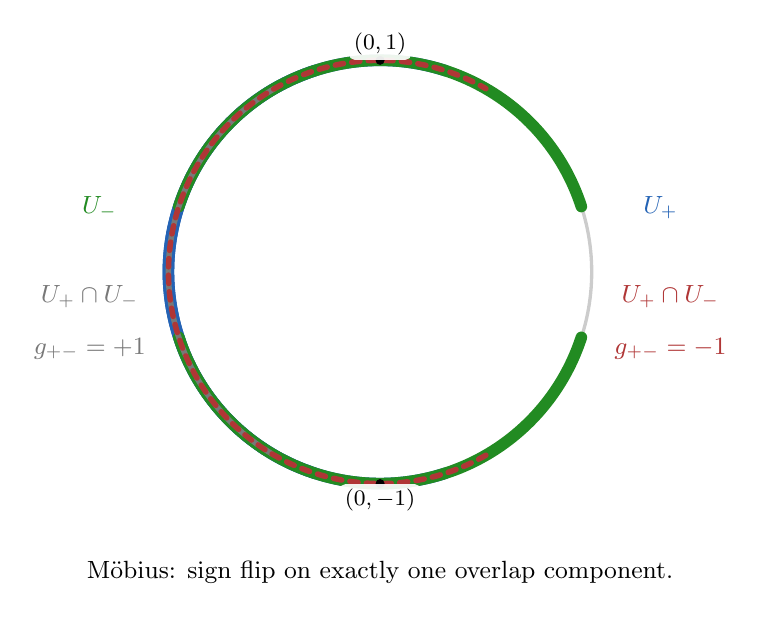
\begin{tikzpicture}[
		scale=1.25,
		line cap=round, line join=round,
		lbl/.style={font=\small, fill=white, fill opacity=0.90, text opacity=1,
			inner sep=2.2pt, rounded corners=2pt},
		labSmall/.style={font=\footnotesize, fill=white, fill opacity=0.92, text opacity=1,
			inner sep=1.8pt, rounded corners=2pt},
		]
		
		% Colors (soft but distinct)
		\definecolor{UplusCol}{RGB}{36,99,181}   % blue
		\definecolor{UminusCol}{RGB}{34,139,34}  % green
		\definecolor{OvPlusCol}{RGB}{120,120,120}% gray
		\definecolor{OvMinusCol}{RGB}{176,54,54} % red
		
		\def\R{2.15}
		\def\gap{18} % degrees: small gaps around the poles
		
		% Base light circle (guide)
		\draw[black!20, line width=1.2pt] (0,0) circle (\R);
		
		% --- U_+ and U_- as thick colored arcs (leave tiny gaps near (0,±1)) ---
		% Mark poles positions at 90° and 270°.
		
		% U_+ : remove poles, draw two arcs (blue)
		\draw[UplusCol, line width=4.2pt]
		({\R*cos(90+\gap)},{\R*sin(90+\gap)}) arc (90+\gap:270-\gap:\R);
		\draw[UplusCol, line width=4.2pt]
		({\R*cos(270+\gap)},{\R*sin(270+\gap)}) arc (270+\gap:90-\gap:\R);
		
		% U_- : another cover (green), rotated so overlap has two components
		\draw[UminusCol, line width=4.2pt]
		({\R*cos(0+\gap)},{\R*sin(0+\gap)}) arc (0+\gap:180-\gap:\R);
		\draw[UminusCol, line width=4.2pt]
		({\R*cos(180+\gap)},{\R*sin(180+\gap)}) arc (180+\gap:360-\gap:\R);
		
		% --- Overlap components highlighted (two dashed arcs) ---
		% Left overlap component (set to +1, gray)
		\draw[OvPlusCol, dashed, line width=2.0pt]
		({\R*cos(120)},{\R*sin(120)}) arc (120:240:\R);
		
		% Right overlap component (set to -1, red)
		\draw[OvMinusCol, dashed, line width=2.0pt]
		({\R*cos(300)},{\R*sin(300)}) arc (300:60:\R);
		
		% Poles
		\fill (0,\R) circle (1.3pt);
		\fill (0,-\R) circle (1.3pt);
		
		\node[labSmall, anchor=south] at (0,\R) {$(0,1)$};
		\node[labSmall, anchor=north] at (0,-\R) {$(0,-1)$};
		
		% Labels for U_+, U_-
		\node[lbl, text=UplusCol]  at (2.85,0.65) {$U_{+}$};
		\node[lbl, text=UminusCol] at (-2.85,0.65) {$U_{-}$};
		
		% Labels for overlap + transitions, placed away from arcs
		\node[lbl, text=OvPlusCol] at (-2.95,-0.25) {$U_{+}\cap U_{-}$};
		\node[lbl, text=OvPlusCol] at (-2.95,-0.78) {$g_{+-}=+1$};
		
		\node[lbl, text=OvMinusCol] at (2.95,-0.25) {$U_{+}\cap U_{-}$};
		\node[lbl, text=OvMinusCol] at (2.95,-0.78) {$g_{+-}=-1$};
		
		% Caption-like note (inside tikz, keeps spacing tight)
		\node[font=\small] at (0,-3.05) {M\"obius: sign flip on exactly one overlap component.};
		
	\end{tikzpicture}
\end{figure}

	
	% Requires: \usepackage{pgfplots}
	% \pgfplotsset{compat=1.18}
	
	\begin{figure}[H]
		\centering
		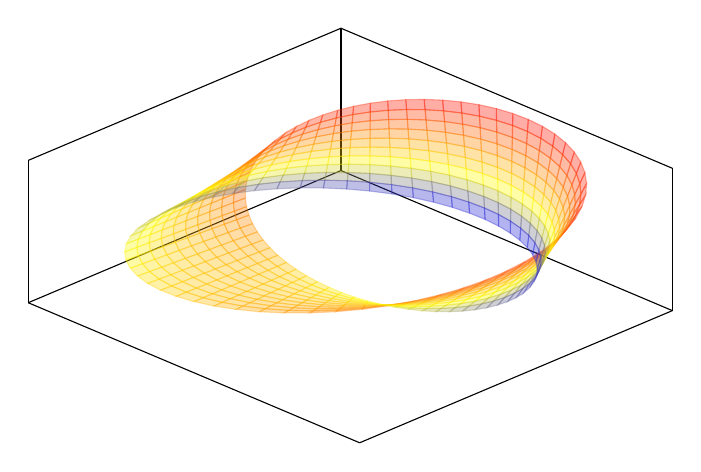
\begin{tikzpicture}
			\begin{axis}[
				view={135}{25},
				axis equal image,
				ticks=none,
				width=10cm, height=7cm,
				]
				% Möbius strip parametrization:
				% u in [0,2pi], v in [-1,1]
				% ( (1 + a v cos(u/2)) cos u, (1 + a v cos(u/2)) sin u, a v sin(u/2) )
				\addplot3[
				surf,
				domain=0:360,
				y domain=-1:1,
				samples=60, samples y=11,
				opacity=0.35,
				shader=flat,
				]
				(
				{(1 + 0.35*y*cos(x/2))*cos(x)},
				{(1 + 0.35*y*cos(x/2))*sin(x)},
				{0.35*y*sin(x/2)}
				);
			\end{axis}
		\end{tikzpicture}
		\caption{The Möbius strip: total space of the Möbius line bundle over $S^1$.}
	\end{figure}
	
	\begin{figure}[H]
		\centering
		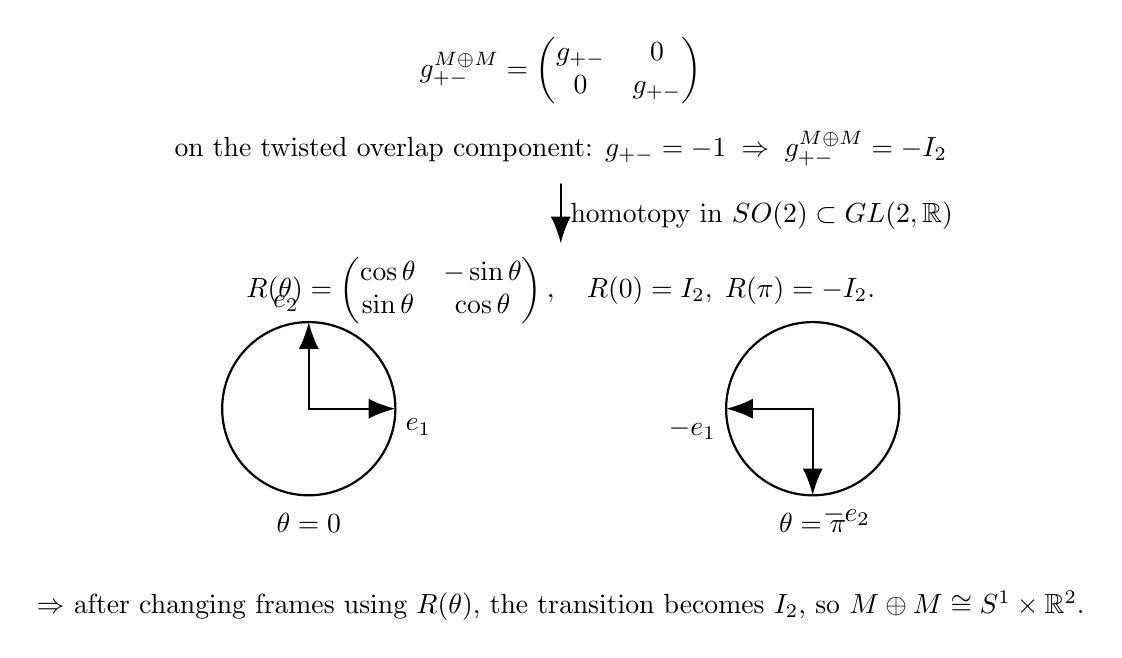
\begin{tikzpicture}[scale=1.0, line cap=round, line join=round]
			\node at (0,0.0) {$g^{M\oplus M}_{+-}=
				\begin{pmatrix} g_{+-} & 0\\ 0 & g_{+-}\end{pmatrix}$};
			
			\node at (0,-1.0) {on the twisted overlap component: $g_{+-}=-1\;\Rightarrow\;g^{M\oplus M}_{+-}=-I_2$};
			
			% Arrow to homotopy
			\draw[->, thick] (0,-1.45) -- (0,-2.2);
			\node[right] at (0,-1.85) {homotopy in $SO(2)\subset GL(2,\mathbb R)$};
			
			% Rotation path
			\node at (0,-2.8) {$R(\theta)=\begin{pmatrix}\cos\theta & -\sin\theta\\ \sin\theta & \cos\theta\end{pmatrix},\quad
				R(0)=I_2,\; R(\pi)=-I_2.$};
			
			% Small schematic: vectors rotating
			\draw[thick] (-3.2,-4.3) circle (1.1);
			\draw[->,thick] (-3.2,-4.3) -- ++(1.1,0) node[below right] {$e_1$};
			\draw[->,thick] (-3.2,-4.3) -- ++(0,1.1) node[above left] {$e_2$};
			
			\draw[thick] (3.2,-4.3) circle (1.1);
			\draw[->,thick] (3.2,-4.3) -- ++(-1.1,0) node[below left] {$-e_1$};
			\draw[->,thick] (3.2,-4.3) -- ++(0,-1.1) node[below right] {$-e_2$};
			
			\node at (-3.2,-5.75) {$\theta=0$};
			\node at (3.2,-5.75) {$\theta=\pi$};
			
			\node at (0,-6.8) {$\Rightarrow$ after changing frames using $R(\theta)$, the transition becomes $I_2$,
				so $M\oplus M\cong S^1\times\mathbb R^2$.};
		\end{tikzpicture}
		\caption{Matrix viewpoint: $g^{M\oplus M}_{+-}=-I_2$ is homotopic to $I_2$ via rotations, hence the rank-2 bundle is trivial.}
	\end{figure}
	
	\begin{figure}[H]
		\centering
		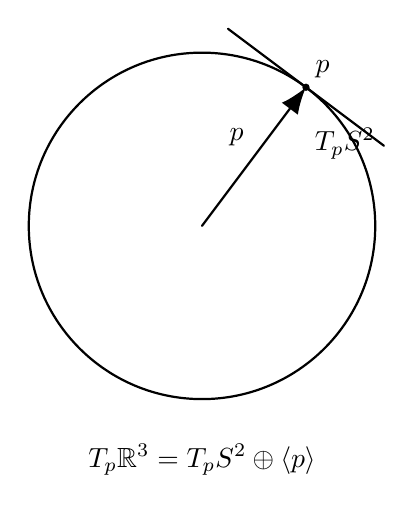
\begin{tikzpicture}[scale=1.1, line cap=round, line join=round]
			% Sphere outline (circle for S^2 schematic)
			\draw[thick] (0,0) circle (2);
			
			% Point p on sphere
			\coordinate (P) at (1.2,1.6);
			\fill (P) circle (1.2pt) node[above right] {$p$};
			
			% Radius/normal vector
			\draw[->, thick] (0,0) -- (P) node[midway, above left] {$p$};
			
			% Tangent line at P (perpendicular to radius)
			% tangent direction vector
			\coordinate (T1) at ($(P)+(-0.9,0.675)$);
			\coordinate (T2) at ($(P)-(-0.9,0.675)$);
			\draw[thick] (T1) -- (T2);
			\node at ($(P)+(0.45,-0.65)$) {$T_pS^2$};
			
			% Little decomposition label
			\node at (0,-2.7) {$T_p\mathbb R^{3}=T_pS^2\oplus \langle p\rangle$};
		\end{tikzpicture}
		\caption{At each $p\in S^n$, the ambient tangent space splits as $T_p\mathbb R^{n+1}=T_pS^n\oplus \langle p\rangle$,
			giving $TS^n\oplus \mathbb R\cong \mathbb R^{n+1}$.}
	\end{figure}
	
	
	% ============================================================
	% Problem 3
	% ============================================================
	\subsection*{Problem 3: Pullback of the tautological bundle under the Hopf map}
	
	\noindent Show that
	\[
	H^*\mathcal O_{\mathbb{CP}^n}(-1) \;\cong\; \mathbb{C},
	\]
	where $H:S^{2n+1}\to \mathbb{CP}^n$ is the Hopf map.
	
	
		% ============================================================
	% Theory for Problem 3
	% ============================================================
	\subsection*{Theory for Problem 3: Pullback of $\mathcal O_{\mathbb{CP}^n}(-1)$ under the Hopf map}
	
	\paragraph{\textbf{Tautological line bundle.}}
	The tautological (universal) complex line bundle over $\mathbb{CP}^n$ is
	\[
	\mathcal O_{\mathbb{CP}^n}(-1)=\{([\ell],v)\in \mathbb{CP}^n\times \mathbb C^{n+1}:\ v\in \ell\}\to \mathbb{CP}^n,
	\]
	whose fibre over $[\ell]\in \mathbb{CP}^n$ is the line $\ell\subset \mathbb C^{n+1}$.
	
	\paragraph{\textbf{Hopf map.}}
	The Hopf map is
	\[
	H:S^{2n+1}\subset \mathbb C^{n+1}\to \mathbb{CP}^n,\qquad H(z)=[z],
	\]
	sending a unit vector $z$ to the complex line it spans.
	
	\paragraph{\textbf{Why the pullback is trivial.}}
	The pullback bundle $H^*\mathcal O_{\mathbb{CP}^n}(-1)\to S^{2n+1}$ has fibre at $z$ equal to
	\[
	(H^*\mathcal O(-1))_z=\mathcal O(-1)_{H(z)}=\mathbb C z.
	\]
	There is a canonical nowhere-zero section
	\[
	s:S^{2n+1}\to H^*\mathcal O(-1),\qquad s(z)=(z,z),
	\]
	since $z\in \mathbb Cz$ and $z\neq 0$ on the unit sphere. A nowhere-zero section of a complex line bundle
	trivialises it, hence
	\[
	H^*\mathcal O_{\mathbb{CP}^n}(-1)\cong S^{2n+1}\times \mathbb C.
	\]
	
	
	% ============================================================
	% Problem 4: Divisibility by a nowhere-zero 1-form
	% ============================================================
	
	\subsection*{Problem 4: Divisibility by a nowhere-zero $1$-form}
	
	\noindent \textbf{Problem statement.}
	Let $\alpha$ be a nowhere-zero $1$-form on a manifold $X$, and let $\beta$ be a $p$-form.
	Show:
	(i) if $\beta=\alpha\wedge\gamma$ for some $(p-1)$-form $\gamma$, then $\alpha\wedge\beta=0$;
	(ii) conversely, if $\alpha\wedge\beta=0$ then there exists a $(p-1)$-form $\gamma$ with $\beta=\alpha\wedge\gamma$
	(hint: work locally, then use a partition of unity);
	(iii) must we have $\beta\wedge\beta=0$?
	
	\medskip
	\noindent \textbf{Solution.}
	\textit{(i)} If $\beta=\alpha\wedge\gamma$, then
	\[
	\alpha\wedge\beta=\alpha\wedge(\alpha\wedge\gamma)=(\alpha\wedge\alpha)\wedge\gamma=0,
	\]
	since $\alpha\wedge\alpha=0$ for every $1$-form $\alpha$.
	
	\smallskip
	\textit{(ii) Local step.}
	Fix $x\in X$. Since $\alpha_x\neq 0$, there is a neighborhood $U\ni x$ and coordinates
	$(x^1,\dots,x^n)$ on $U$ such that
	\[
	\alpha|_U=dx^1.
	\]
	Write $\beta$ uniquely on $U$ as
	\[
	\beta = dx^1\wedge \eta + \zeta,
	\]
	where $\eta$ is a $(p-1)$-form on $U$ and $\zeta$ is a $p$-form involving only
	$dx^2,\dots,dx^n$ (equivalently, $\iota_{\partial_{x^1}}\zeta=0$).
	Then
	\[
	dx^1\wedge\beta = dx^1\wedge(dx^1\wedge\eta+\zeta)=dx^1\wedge\zeta.
	\]
	If $dx^1\wedge\beta=0$, then $dx^1\wedge\zeta=0$. Expanding in the basis wedges
	$dx^1\wedge dx^{i_1}\wedge\cdots\wedge dx^{i_p}$ with $i_j\ge 2$ shows all coefficients vanish,
	hence $\zeta=0$. Therefore on $U$,
	\[
	\beta = dx^1\wedge\eta = \alpha\wedge\eta.
	\]
	So locally $\beta=\alpha\wedge\gamma_U$ with $\gamma_U:=\eta$.
	
	\smallskip
	\textit{(ii) Global step (partition of unity).}
	Choose an open cover $\{U_i\}$ such that $\beta|_{U_i}=\alpha\wedge\gamma_i$ for some $(p-1)$-forms $\gamma_i$.
	Let $\{\varphi_i\}$ be a partition of unity subordinate to $\{U_i\}$ and define
	\[
	\gamma := \sum_i \varphi_i\,\gamma_i.
	\]
	Then
	\[
	\alpha\wedge\gamma
	= \sum_i \alpha\wedge(\varphi_i\gamma_i)
	= \sum_i \varphi_i(\alpha\wedge\gamma_i)
	= \sum_i \varphi_i\,\beta
	= \beta,
	\]
	so $\beta=\alpha\wedge\gamma$ globally.
	
	\smallskip
	\textit{(iii)} Yes. By (ii) we can write $\beta=\alpha\wedge\gamma$, hence
	\[
	\beta\wedge\beta = (\alpha\wedge\gamma)\wedge(\alpha\wedge\gamma)
	= \alpha\wedge\alpha\wedge\gamma\wedge\gamma=0.
	\]
	(Also, if $p$ is odd then $\beta\wedge\beta=0$ for any $p$-form by graded commutativity.)
	
	
	
	
	% ============================================================
	% Problem 5: de Rham cohomology of spheres via U_±
	% ============================================================
	
	% ============================================================
	% Theory: Problem 4 (nowhere-zero 1-form and divisibility)
	% ============================================================
	
	\subsection*{Theory for Problem 4: Nowhere-zero $1$-forms and ``divisibility''}
	
	\paragraph{Wedge product basics.}
	For differential forms the wedge product is bilinear and alternating. In particular, for any $1$-form $\alpha$,
	\[
	\alpha\wedge\alpha=0.
	\]
	More generally, for $\omega\in\Omega^p(X)$ and $\eta\in\Omega^q(X)$ one has graded commutativity
	\[
	\omega\wedge\eta = (-1)^{pq}\,\eta\wedge\omega.
	\]
	Hence if $p$ is odd then $\omega\wedge\omega=0$ for every $p$-form $\omega$.
	
	\paragraph{A nowhere-zero $1$-form defines a line subbundle.}
	A nowhere-zero $1$-form $\alpha\in\Omega^1(X)$ means $\alpha_x\neq 0\in T_x^*X$ for all $x\in X$.
	Pointwise, the line $\langle \alpha_x\rangle\subset T_x^*X$ varies smoothly with $x$ and defines a rank-$1$ subbundle
	\[
	L:=\langle \alpha\rangle \subset T^*X.
	\]
	Equivalently, $\ker(\alpha_x)\subset T_xX$ is a codimension-$1$ hyperplane distribution.
	
	\paragraph{The pointwise linear-algebra lemma.}
	Let $V$ be a real vector space and let $\alpha\in V^*$ be nonzero. Consider the linear map
	\[
	\alpha\wedge(\cdot):\Lambda^p V^* \longrightarrow \Lambda^{p+1}V^*.
	\]
	Then
	\[
	\mathrm{im}\big(\alpha\wedge:\Lambda^{p-1}V^*\to\Lambda^{p}V^*\big)
	\;\subseteq\;
	\ker\big(\alpha\wedge:\Lambda^{p}V^*\to\Lambda^{p+1}V^*\big),
	\]
	since $\alpha\wedge(\alpha\wedge\gamma)=0$.
	Moreover, for $\alpha\neq 0$ one has the exactness identity
	\[
	\ker\big(\alpha\wedge:\Lambda^{p}V^*\to\Lambda^{p+1}V^*\big)
	\;=\;
	\mathrm{im}\big(\alpha\wedge:\Lambda^{p-1}V^*\to\Lambda^{p}V^*\big).
	\]
	Equivalently,
	\[
	\alpha\wedge\beta=0
	\quad\Longleftrightarrow\quad
	\beta=\alpha\wedge\gamma \text{ for some }\gamma\in\Lambda^{p-1}V^*.
	\]
	
	\paragraph{Proof idea of the lemma (splitting).}
	Choose a basis $(e^1,\dots,e^n)$ of $V^*$ with $\alpha=e^1$. Every $\beta\in\Lambda^pV^*$ decomposes uniquely as
	\[
	\beta = e^1\wedge\eta + \zeta,
	\]
	where $\eta\in\Lambda^{p-1}V^*$ and $\zeta\in\Lambda^p(\mathrm{span}\{e^2,\dots,e^n\})$ (i.e.\ $\zeta$ has no $e^1$ factor).
	Then
	\[
	e^1\wedge\beta = e^1\wedge\zeta.
	\]
	But $e^1\wedge\zeta=0$ forces $\zeta=0$ by linear independence of the basis wedges containing $e^1$, hence
	$\beta=e^1\wedge\eta$.
	
	\paragraph{Local normal form on manifolds.}
	On a manifold, the basis choice ``$\alpha=e^1$'' becomes a local coframe choice:
	for each $x\in X$ with $\alpha_x\neq 0$, there is a neighborhood $U$ and a local coframe
	$(\theta^1,\dots,\theta^n)$ on $U$ such that
	\[
	\alpha|_U = \theta^1.
	\]
	With respect to this coframe, the pointwise splitting above shows that $\alpha\wedge\beta=0$ on $U$
	implies $\beta=\alpha\wedge\gamma_U$ for some local $(p-1)$-form $\gamma_U$.
	
	\paragraph{Patching with a partition of unity.}
	If $\{U_i\}$ is an open cover and $\beta|_{U_i}=\alpha\wedge\gamma_i$, then for a partition of unity
	$\{\varphi_i\}$ subordinate to $\{U_i\}$ the global form
	\[
	\gamma := \sum_i \varphi_i\,\gamma_i
	\]
	satisfies
	\[
	\alpha\wedge\gamma
	= \sum_i \alpha\wedge(\varphi_i\gamma_i)
	= \sum_i \varphi_i(\alpha\wedge\gamma_i)
	= \sum_i \varphi_i\,\beta
	= \beta.
	\]
	
	\paragraph{Remark on $\beta\wedge\beta$.}
	If $p$ is odd then $\beta\wedge\beta=0$ for every $p$-form $\beta$ by graded commutativity.
	In the situation of Problem~4, if $\alpha\wedge\beta=0$ and $\alpha$ is nowhere-zero, then $\beta=\alpha\wedge\gamma$,
	so
	\[
	\beta\wedge\beta = (\alpha\wedge\gamma)\wedge(\alpha\wedge\gamma)
	= \alpha\wedge\alpha\wedge\gamma\wedge\gamma=0
	\]
	regardless of the parity of $p$.
	
	
	
% ============================================================
% Chart: Problem 4 (decomposition beta = alpha^eta + zeta)
% ============================================================
\begin{figure}[H]
	\centering
	\resizebox{0.98\textwidth}{!}{%
		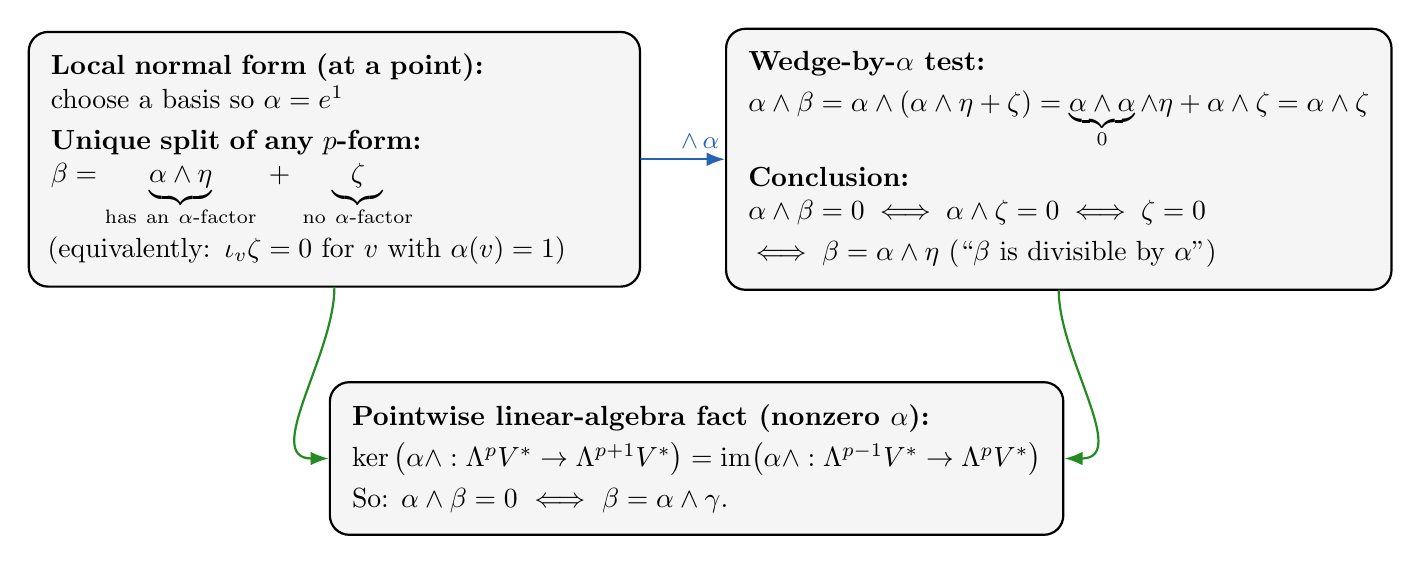
\begin{tikzpicture}[>=Latex, line cap=round, line join=round]
			
			% Colors (soft + readable)
			\definecolor{blueA}{RGB}{36,99,181}
			\definecolor{greenA}{RGB}{34,139,34}
			\definecolor{redA}{RGB}{176,54,54}
			\definecolor{grayB}{RGB}{245,245,245}
			
			\tikzset{
				box/.style={rounded corners=7pt, draw=black, thick, fill=grayB, inner sep=8pt, align=left},
				arrowB/.style={->, thick, draw=blueA},
				arrowG/.style={->, thick, draw=greenA},
				arrowR/.style={->, thick, draw=redA},
				lab/.style={align=center, font=\small},
			}
			
			% --- Left: decomposition
			\node[box, text width=7.2cm, align=left] (decomp) at (0,0) {%
				\textbf{Local normal form (at a point):}\\
				choose a basis so $\alpha=e^1$\\[1mm]
				\textbf{Unique split of any $p$-form:}\\
				$\displaystyle \beta = \underbrace{\alpha\wedge \eta}_{\text{has an }\alpha\text{-factor}}
				\;+\;
				\underbrace{\zeta}_{\text{no }\alpha\text{-factor}}$\\[1mm]
				(equivalently: $\iota_{v}\zeta=0$ for $v$ with $\alpha(v)=1$)
			};
			
			% --- Right: wedge test
			\node[box] (wedge) at (9.2,0) {%
				\textbf{Wedge-by-$\alpha$ test:}\\[1mm]
				$\displaystyle \alpha\wedge\beta
				= \alpha\wedge(\alpha\wedge\eta+\zeta)
				= \underbrace{\alpha\wedge\alpha}_{0}\wedge\eta + \alpha\wedge\zeta
				= \alpha\wedge\zeta$\\[2mm]
				\textbf{Conclusion:}\\
				$\alpha\wedge\beta=0 \iff \alpha\wedge\zeta=0 \iff \zeta=0$\\[1mm]
				$\iff \beta=\alpha\wedge\eta$ (``$\beta$ is divisible by $\alpha$'')
			};
			
			\draw[arrowB] (decomp.east) -- node[lab, above, text=blueA] {$\ \ \ \ \wedge\,\alpha$} (wedge.west);
			
			% --- Bottom: kernel = image picture (MOVED LOWER)
			\node[box] (exact) at (4.6,-3.8) {%
				\textbf{Pointwise linear-algebra fact (nonzero $\alpha$):}\\[1mm]
				$\ker\big(\alpha\wedge:\Lambda^pV^*\to\Lambda^{p+1}V^*\big)
				=
				\mathrm{im}\big(\alpha\wedge:\Lambda^{p-1}V^*\to\Lambda^{p}V^*\big)$\\[1mm]
				So: $\alpha\wedge\beta=0 \ \Longleftrightarrow\ \beta=\alpha\wedge\gamma$.
			};
			
			\draw[arrowG] (wedge.south) to[out=-90,in=0] (exact.east);
			\draw[arrowG] (decomp.south) to[out=-90,in=180] (exact.west);
			
		\end{tikzpicture}%
	}
	\caption{Problem 4: the local decomposition $\beta=\alpha\wedge\eta+\zeta$ and why $\alpha\wedge\beta=0$ forces $\zeta=0$.}
\end{figure}


% ============================================================
% Differential forms: 1-forms and p-forms (definitions + examples)
% Sphere and cone examples + Green/Stokes link
% ============================================================

\subsection*{Differential forms: 1-forms and $p$-forms (with examples on $S^2$ and a cone)}

\paragraph{Tangent spaces and cotangent spaces.}
Let $M$ be a smooth manifold and $x\in M$.
The \emph{tangent space} $T_xM$ is the vector space of tangent vectors at $x$.
The \emph{cotangent space} at $x$ is the dual space
\[
T_x^*M := \mathrm{Hom}(T_xM,\mathbb{R}),
\]
the space of linear functionals on $T_xM$.

\paragraph{1-forms.}
A \emph{(smooth) 1-form} on $M$ is a smooth assignment
\[
\alpha: x \mapsto \alpha_x \in T_x^*M,
\]
so that for each $x$, $\alpha_x: T_xM \to \mathbb{R}$ is linear and depends smoothly on $x$.
Equivalently, a 1-form is a smooth covector field.

In local coordinates $(x^1,\dots,x^n)$ on an open set $U\subset M$, every 1-form has the form
\[
\alpha = \sum_{i=1}^n a_i(x)\, dx^i,
\]
where $a_i\in C^\infty(U)$ and $dx^i$ are the coordinate 1-forms characterized by
$dx^i\!\left(\frac{\partial}{\partial x^j}\right)=\delta^i_j$.

\paragraph{Example in $\mathbb{R}^2$.}
A standard 1-form is
\[
\alpha = P(x,y)\,dx + Q(x,y)\,dy,
\]
where $P,Q$ are smooth functions. If $v=(v_x,v_y)\in T_{(x,y)}\mathbb{R}^2\cong\mathbb{R}^2$, then
\[
\alpha_{(x,y)}(v)=P(x,y)\,v_x + Q(x,y)\,v_y.
\]

\paragraph{Line integrals of 1-forms.}
If $\gamma:[a,b]\to M$ is a smooth curve, the integral of a 1-form along $\gamma$ is defined by pullback:
\[
\int_\gamma \alpha := \int_a^b \gamma^*\alpha.
\]
In coordinates, if $\alpha=P\,dx+Q\,dy$ and $\gamma(t)=(x(t),y(t))$, then
\[
\gamma^*\alpha = P(x(t),y(t))\,x'(t)\,dt + Q(x(t),y(t))\,y'(t)\,dt,
\]
hence
\[
\int_\gamma \alpha = \int_a^b \Big(P(x(t),y(t))x'(t)+Q(x(t),y(t))y'(t)\Big)\,dt.
\]

\paragraph{$p$-forms.}
A \emph{$p$-form} on $M$ is a smooth assignment
\[
\omega: x \mapsto \omega_x \in \Lambda^p(T_x^*M),
\]
where $\Lambda^p(T_x^*M)$ is the space of alternating $p$-linear maps
\[
\omega_x:\underbrace{T_xM\times\cdots\times T_xM}_{p\ \text{times}} \to \mathbb{R}.
\]
Alternating means that swapping two inputs changes the sign; in particular, if two input vectors coincide,
the value is $0$.

In local coordinates $(x^1,\dots,x^n)$, every $p$-form can be written as
\[
\omega = \sum_{i_1<\cdots<i_p} a_{i_1\cdots i_p}(x)\, dx^{i_1}\wedge\cdots\wedge dx^{i_p},
\]
where the wedge product $\wedge$ encodes alternation.

\paragraph{What you integrate.}
A $1$-form integrates over $1$-dimensional objects (curves), a $2$-form integrates over surfaces,
and in general a $p$-form integrates over oriented $p$-dimensional submanifolds (or $p$-chains).
An $n$-form on an $n$-manifold is a \emph{volume form} (locally it looks like a density times
$dx^1\wedge\cdots\wedge dx^n$).

\paragraph{Examples in $\mathbb{R}^3$.}
Using coordinates $(x,y,z)$, typical examples are:
\[
\text{1-form: } \alpha = x\,dx + y\,dy + z\,dz,\qquad
\text{2-form: } dx\wedge dy,\qquad
\text{3-form: } dx\wedge dy\wedge dz.
\]
The 2-form $dx\wedge dy$ measures oriented area in the $xy$-plane, while $dx\wedge dy\wedge dz$
is the standard oriented volume form.

% ------------------------------------------------------------
% Sphere examples
% ------------------------------------------------------------
\subsubsection*{Examples on the sphere $S^2$}

\paragraph{A 1-form on $S^2$ via restriction from $\mathbb{R}^3$.}
Let $\iota:S^2\hookrightarrow \mathbb{R}^3$ be the inclusion, with ambient coordinates $(x,y,z)$.
Consider the 1-form on $\mathbb{R}^3$
\[
\beta = -y\,dx + x\,dy.
\]
Define a 1-form on $S^2$ by restriction (pullback):
\[
\alpha := \iota^*\beta.
\]
This 1-form measures ``rotation'' around the $z$-axis.

\paragraph{Integral of $\alpha$ along a latitude circle.}
Fix $z_0\in(-1,1)$ and let $r=\sqrt{1-z_0^2}$. The latitude circle at height $z=z_0$ is
\[
\gamma(t)=(r\cos t,\ r\sin t,\ z_0),\qquad t\in[0,2\pi].
\]
Along $\gamma$ we have
\[
dx = -r\sin t\,dt,\qquad dy = r\cos t\,dt,
\]
and thus
\[
\beta(\gamma'(t))\,dt = \big(-y\,dx + x\,dy\big)\Big|_{\gamma(t)}
= -(r\sin t)(-r\sin t\,dt) + (r\cos t)(r\cos t\,dt)=r^2\,dt.
\]
Hence
\[
\int_\gamma \alpha = \int_\gamma \iota^*\beta = \int_0^{2\pi} r^2\,dt
= 2\pi r^2 = 2\pi(1-z_0^2).
\]

\paragraph{The standard area 2-form on $S^2$.}
In spherical coordinates $(\theta,\phi)$ (colatitude $\theta\in(0,\pi)$ and longitude $\phi\in(0,2\pi)$),
the standard area form is
\[
\omega_{S^2} = \sin\theta\, d\theta\wedge d\phi.
\]
Its total integral gives the surface area of the unit sphere:
\[
\int_{S^2}\omega_{S^2} = 4\pi.
\]

% ------------------------------------------------------------
% Cone examples
% ------------------------------------------------------------
\subsubsection*{Examples on a cone (via parametrization)}

\paragraph{Cone parametrization.}
Consider the cone in $\mathbb{R}^3$ (without the tip) parametrized by
\[
F(r,\theta)=(r\cos\theta,\ r\sin\theta,\ a r),
\qquad r>0,\ \theta\in[0,2\pi),
\]
where $a>0$ controls the slope.

\paragraph{Pulling back the rotation 1-form $\beta=-y\,dx+x\,dy$.}
Let $\beta=-y\,dx + x\,dy$ on $\mathbb{R}^3$. We compute $F^*\beta$.
Along $F$ we have
\[
x=r\cos\theta,\qquad y=r\sin\theta,
\]
and
\[
dx=\cos\theta\,dr - r\sin\theta\,d\theta,\qquad
dy=\sin\theta\,dr + r\cos\theta\,d\theta.
\]
Therefore
\begin{align*}
	F^*\beta
	&= -(r\sin\theta)\,dx + (r\cos\theta)\,dy \\
	&= -(r\sin\theta)\big(\cos\theta\,dr - r\sin\theta\,d\theta\big)
	+ (r\cos\theta)\big(\sin\theta\,dr + r\cos\theta\,d\theta\big) \\
	&= \big(-r\sin\theta\cos\theta + r\cos\theta\sin\theta\big)\,dr
	+ r^2(\sin^2\theta+\cos^2\theta)\,d\theta \\
	&= r^2\,d\theta.
\end{align*}
In particular, for the circle $r=r_0$ (with $\theta$ running from $0$ to $2\pi$),
\[
\int_{r=r_0} F^*\beta = \int_0^{2\pi} r_0^2\,d\theta = 2\pi r_0^2.
\]

\paragraph{A natural area 2-form on the cone.}
The induced surface area element is
\[
\|F_r\times F_\theta\|\,dr\wedge d\theta.
\]
Here
\[
F_r=(\cos\theta,\ \sin\theta,\ a),\qquad
F_\theta=(-r\sin\theta,\ r\cos\theta,\ 0),
\]
and one computes
\[
\|F_r\times F_\theta\| = r\sqrt{1+a^2}.
\]
Hence an area 2-form on the cone is
\[
\omega_{\mathrm{cone}} = r\sqrt{1+a^2}\, dr\wedge d\theta.
\]
Integrating over a frustum region $r\in[r_1,r_2]$, $\theta\in[0,2\pi]$ gives the lateral area:
\[
\int_{r_1}^{r_2}\int_0^{2\pi} r\sqrt{1+a^2}\, d\theta\,dr
= \pi\sqrt{1+a^2}\,(r_2^2-r_1^2).
\]

% ------------------------------------------------------------
% Stokes/Green link
% ------------------------------------------------------------
\subsubsection*{Exterior derivative and the Green/Stokes connection}

\paragraph{Exterior derivative on a 1-form in $\mathbb{R}^2$.}
Let $\alpha=P\,dx+Q\,dy$ on an open set in $\mathbb{R}^2$. Then
\[
d\alpha = d(P\,dx)+d(Q\,dy)=dP\wedge dx + dQ\wedge dy.
\]
Writing $dP=P_x\,dx+P_y\,dy$ and $dQ=Q_x\,dx+Q_y\,dy$ gives
\[
d\alpha = (P_x\,dx+P_y\,dy)\wedge dx + (Q_x\,dx+Q_y\,dy)\wedge dy
= P_y\,dy\wedge dx + Q_x\,dx\wedge dy.
\]
Since $dy\wedge dx=-dx\wedge dy$, we obtain
\[
d\alpha = \left(\frac{\partial Q}{\partial x}-\frac{\partial P}{\partial y}\right)\,dx\wedge dy.
\]

\paragraph{Stokes' theorem (Green's theorem as a special case).}
If $\Omega\subset\mathbb{R}^2$ is a compact region with smooth boundary $\partial\Omega$
(or more generally a compact oriented $2$-manifold-with-boundary),
Stokes' theorem says
\[
\int_{\partial\Omega}\alpha = \int_{\Omega} d\alpha.
\]
With the formula above for $d\alpha$, this becomes the classical Green's theorem:
\[
\int_{\partial\Omega} (P\,dx+Q\,dy)
=
\int_{\Omega} \left(\frac{\partial Q}{\partial x}-\frac{\partial P}{\partial y}\right)\,dx\,dy.
\]

% ============================================================
% Calculus vs differential forms: dy, y'(x), building 1-forms and p-forms
% Extended explanation + many examples + pullback viewpoint
% ============================================================

\subsection*{From calculus to differential forms: $dy$, $y'(x)=\frac{dy}{dx}$, and building $1$- and $p$-forms}

\paragraph{0-forms, 1-forms, $p$-forms.}
A \emph{$0$-form} on a manifold $M$ is just a smooth function $f\in C^\infty(M)$.
A \emph{$1$-form} is a smooth covector field $\alpha\in\Omega^1(M)$, i.e.\ for each $x\in M$,
\[
\alpha_x \in T_x^*M=\mathrm{Hom}(T_xM,\mathbb{R}).
\]
More generally, a \emph{$p$-form} $\omega\in\Omega^p(M)$ assigns to each $x\in M$ an alternating multilinear map
\[
\omega_x : \underbrace{T_xM\times\cdots\times T_xM}_{p\ \text{times}} \to \mathbb{R},
\qquad \omega_x \in \Lambda^p(T_x^*M).
\]
Alternating means swapping two arguments changes sign; in particular, if two arguments coincide then the value is $0$.

\subsubsection*{The differential $df$ is a 1-form}

\paragraph{Definition of the differential.}
Let $f\in C^\infty(M)$ be a smooth function. Its \emph{differential} (or \emph{exterior derivative} in degree $0$)
is the 1-form $df\in\Omega^1(M)$ defined by
\[
(df)_x(v) := v(f)\qquad \text{for }x\in M,\ v\in T_xM,
\]
where $v(f)$ denotes the directional derivative of $f$ along the tangent vector $v$.

\paragraph{Coordinate formula.}
On a coordinate chart $(U; x^1,\dots,x^n)$, any tangent vector at $x\in U$ can be written
\[
v=\sum_{i=1}^n v^i \frac{\partial}{\partial x^i}\Big|_x.
\]
Then
\[
(df)_x(v)=\sum_{i=1}^n v^i \frac{\partial f}{\partial x^i}(x),
\]
so as a 1-form we have the standard expression
\[
df=\sum_{i=1}^n \frac{\partial f}{\partial x^i}\,dx^i.
\]

\subsubsection*{Why $dy$ is a 1-form, and how it relates to $y'(x)=\frac{dy}{dx}$}

\paragraph{One-dimensional case ($M=\mathbb{R}$).}
Let $x$ be the coordinate on $\mathbb{R}$ and let $y=y(x)$ be a smooth function.
Then $y'(x)=\frac{dy}{dx}$ is a \emph{number} depending on $x$ (a $0$-form).
The symbol $dy$ is the \emph{differential} of the function $y$, hence a \emph{1-form}:
\[
dy = d(y) \in \Omega^1(\mathbb{R}).
\]
By the coordinate formula,
\[
dy = \frac{dy}{dx}\,dx = y'(x)\,dx.
\]
This is the precise relationship:
\begin{itemize}
	\item $y'(x)$ is a scalar function (a $0$-form),
	\item $dx$ is the basic 1-form on $\mathbb{R}$,
	\item $dy$ is a 1-form obtained as their product.
\end{itemize}

\paragraph{Evaluation on a tangent vector.}
In $T_x\mathbb{R}$, the canonical basis vector is $\frac{\partial}{\partial x}\big|_x$.
Evaluating $dy$ on it recovers the usual derivative:
\[
dy\!\left(\frac{\partial}{\partial x}\right)=\frac{dy}{dx}=y'(x).
\]
More generally, if $v=a\,\frac{\partial}{\partial x}$, then
\[
dy(v)=a\,y'(x).
\]
So \emph{a 1-form is something you feed a tangent vector to obtain a number.}

\subsubsection*{Differentials $dx$, $dy$ in $\mathbb{R}^2$ and the meaning of $\frac{dy}{dx}$}

\paragraph{Basic 1-forms on $\mathbb{R}^2$.}
In $\mathbb{R}^2$ with coordinates $(x,y)$, the coordinate 1-forms $dx$ and $dy$ satisfy
\[
dx\!\left(\frac{\partial}{\partial x}\right)=1,\quad dx\!\left(\frac{\partial}{\partial y}\right)=0,
\qquad
dy\!\left(\frac{\partial}{\partial x}\right)=0,\quad dy\!\left(\frac{\partial}{\partial y}\right)=1.
\]
A general 1-form is
\[
\alpha = P(x,y)\,dx + Q(x,y)\,dy,
\]
and it acts on a tangent vector $v=v^x\frac{\partial}{\partial x}+v^y\frac{\partial}{\partial y}$ by
\[
\alpha(v)=P(x,y)\,v^x + Q(x,y)\,v^y.
\]

\paragraph{Differential of a function in $\mathbb{R}^2$.}
If $f=f(x,y)$ then
\[
df=f_x\,dx+f_y\,dy.
\]

\paragraph{The ratio $\frac{dy}{dx}$ along a parametrized curve.}
Let $\gamma(t)=(x(t),y(t))$ be a smooth curve with $x'(t)\neq 0$.
Then $\gamma'(t)\in T_{\gamma(t)}\mathbb{R}^2$ and
\[
dx(\gamma'(t))=\frac{d}{dt}(x(t))=x'(t),
\qquad
dy(\gamma'(t))=\frac{d}{dt}(y(t))=y'(t).
\]
Hence the classical slope is the ratio of evaluations of 1-forms on the same tangent vector:
\[
\frac{dy}{dx}\Big|_{\gamma(t)}=\frac{dy(\gamma'(t))}{dx(\gamma'(t))}=\frac{y'(t)}{x'(t)}.
\]
This explains conceptually why $dx$ and $dy$ are fundamental and $\frac{dy}{dx}$ is derived from them.

\subsubsection*{How to build 1-forms directly from calculus data}

\paragraph{Recipe for 1-forms.}
In coordinates $(x^1,\dots,x^n)$, any expression of the form
\[
\alpha = \sum_{i=1}^n a_i(x)\,dx^i
\]
is a 1-form, where the coefficients $a_i$ are smooth functions.

\paragraph{Examples.}
On $\mathbb{R}$: $\alpha=f(x)\,dx$. \\
On $\mathbb{R}^2$: $\alpha=P(x,y)\,dx+Q(x,y)\,dy$. \\
On $\mathbb{R}^3$: $\alpha = x\,dx+y\,dy+z\,dz$.

\subsubsection*{How to build $p$-forms: wedge products}

\paragraph{Wedge product and alternation.}
Given 1-forms $\alpha,\beta\in\Omega^1(M)$, their wedge product $\alpha\wedge\beta\in\Omega^2(M)$ is an alternating
bilinear form. It satisfies
\[
\alpha\wedge\beta = -\,\beta\wedge\alpha,\qquad \alpha\wedge\alpha=0.
\]
In coordinates, a basis for $p$-forms is given by wedges of the coordinate 1-forms:
\[
dx^{i_1}\wedge\cdots\wedge dx^{i_p}\qquad (i_1<\cdots<i_p).
\]

\paragraph{Typical $2$-forms and $3$-forms in Euclidean space.}
In $\mathbb{R}^2$, a general 2-form looks like
\[
\omega = f(x,y)\,dx\wedge dy,
\]
and in $\mathbb{R}^3$, a general 3-form looks like
\[
\eta = g(x,y,z)\,dx\wedge dy\wedge dz.
\]
The 2-form $dx\wedge dy$ represents oriented area density in the plane, and $dx\wedge dy\wedge dz$
represents oriented volume density in $\mathbb{R}^3$.

\subsubsection*{A fundamental example: $du\wedge dv$ and the Jacobian determinant}

\paragraph{Two functions define a 2-form.}
Let $u=u(x,y)$ and $v=v(x,y)$ be smooth functions on $\mathbb{R}^2$. Then $du$ and $dv$ are 1-forms and
$du\wedge dv$ is a 2-form.

Compute in coordinates:
\[
du=u_x\,dx+u_y\,dy,\qquad dv=v_x\,dx+v_y\,dy.
\]
Then
\begin{align*}
	du\wedge dv
	&=(u_x\,dx+u_y\,dy)\wedge(v_x\,dx+v_y\,dy) \\
	&=u_xv_y\,dx\wedge dy + u_yv_x\,dy\wedge dx \\
	&=(u_xv_y-u_yv_x)\,dx\wedge dy.
\end{align*}
The coefficient $u_xv_y-u_yv_x$ is the Jacobian determinant
\[
\det\begin{pmatrix}u_x & u_y\\ v_x & v_y\end{pmatrix}.
\]
Thus wedge products naturally produce determinants, which is why differential forms encode change-of-variables
and orientation very efficiently.

\subsubsection*{Pullback viewpoint: forms along curves and surfaces}

\paragraph{Pullback of a 1-form to a curve (line integrals).}
If $\alpha$ is a 1-form on $M$ and $\gamma:[a,b]\to M$ is a smooth curve, then $\gamma^*\alpha$ is a 1-form on $[a,b]$,
hence of the form $h(t)\,dt$, and we define
\[
\int_\gamma \alpha := \int_a^b \gamma^*\alpha.
\]
In $\mathbb{R}^2$, for $\alpha=P\,dx+Q\,dy$ and $\gamma(t)=(x(t),y(t))$,
\[
\gamma^*\alpha = \big(P(x(t),y(t))x'(t)+Q(x(t),y(t))y'(t)\big)\,dt,
\]
so
\[
\int_\gamma \alpha = \int_a^b \big(P(x(t),y(t))x'(t)+Q(x(t),y(t))y'(t)\big)\,dt.
\]

\paragraph{Pullback of a 2-form to a parametrized surface.}
If $\omega$ is a 2-form on $\mathbb{R}^3$ and $F:U\subset\mathbb{R}^2\to \mathbb{R}^3$ parametrizes a surface,
then $F^*\omega$ is a 2-form on $U$ and can be integrated over $U$.

\subsubsection*{Exterior derivative in degree 1 and Green/Stokes link (calculus to geometry)}

\paragraph{Exterior derivative of a planar 1-form.}
Let $\alpha=P\,dx+Q\,dy$ on an open set in $\mathbb{R}^2$. Then
\[
d\alpha = \left(\frac{\partial Q}{\partial x}-\frac{\partial P}{\partial y}\right)\,dx\wedge dy.
\]
This is a coordinate computation using $d(dx)=d(dy)=0$ and the product rule.

\paragraph{Stokes' theorem (Green's theorem as a special case).}
If $\Omega\subset\mathbb{R}^2$ is a compact region with smooth boundary $\partial\Omega$ (or, more generally, a compact
oriented $2$-manifold-with-boundary), Stokes' theorem states
\[
\int_{\partial\Omega}\alpha = \int_{\Omega} d\alpha.
\]
Substituting the formula for $d\alpha$ yields the classical Green's theorem:
\[
\int_{\partial\Omega} (P\,dx+Q\,dy)
=
\int_{\Omega} \left(\frac{\partial Q}{\partial x}-\frac{\partial P}{\partial y}\right)\,dx\,dy.
\]

\subsubsection*{Summary (calculus dictionary)}
\begin{itemize}
	\item A function $f$ is a $0$-form.
	\item Its differential $df$ is a $1$-form.
	\item In one variable, $dy = y'(x)\,dx$ and $y'(x)=dy\!\left(\frac{\partial}{\partial x}\right)$.
	\item A general $1$-form looks like $\sum a_i\,dx^i$ and integrates along curves.
	\item A general $p$-form is built from wedge products of $1$-forms and integrates over $p$-dimensional oriented domains.
	\item Wedge products encode determinants (Jacobians), and $d(Pdx+Qdy)$ encodes the curl term in Green's theorem.
\end{itemize}

	
% ============================================================
% Sphere S^2: tangent spaces, charts/coordinates, and forms
% + simple TikZ charts
% ============================================================

\subsection*{The sphere $S^2$: tangent spaces and local coordinates (charts)}

\paragraph{Sphere as a submanifold of $\mathbb{R}^3$.}
Consider the unit sphere
\[
S^2=\{(x,y,z)\in\mathbb{R}^3:\ x^2+y^2+z^2=1\}.
\]
It is a smooth $2$-dimensional manifold embedded in $\mathbb{R}^3$.

\paragraph{Tangent space at a point.}
Let $p\in S^2$. A convenient characterization of the tangent space is
\[
T_pS^2=\{v\in\mathbb{R}^3:\ v\cdot p=0\}.
\]
That is, tangent vectors are precisely those vectors orthogonal to the radius vector at $p$.

\paragraph{Example at the north pole.}
At $N=(0,0,1)$ we have
\[
T_NS^2=\{(a,b,c)\in\mathbb{R}^3:\ c=0\},
\]
the $xy$-plane.

\subsection*{Why we need charts: no single global coordinate system on $S^2$}

\paragraph{Local coordinates (charts).}
A \emph{chart} on $S^2$ is a diffeomorphism from an open set $U\subset S^2$ to an open set in $\mathbb{R}^2$.
One cannot cover all of $S^2$ by a single smooth chart; instead one uses a collection of charts whose domains cover $S^2$.

\subsection*{(A) Spherical coordinates $(\theta,\phi)$}

\paragraph{Parametrization.}
Define
\[
F(\theta,\phi)=(\sin\theta\cos\phi,\ \sin\theta\sin\phi,\ \cos\theta),
\qquad 0<\theta<\pi,\ \ 0<\phi<2\pi.
\]
This parametrizes $S^2$ minus the north and south poles (where $\phi$ is not well-defined).

\paragraph{Tangent basis from the parametrization.}
At $p=F(\theta,\phi)$, the partial derivatives span the tangent plane:
\[
F_\theta(\theta,\phi),\quad F_\phi(\theta,\phi)\ \in\ T_{F(\theta,\phi)}S^2,
\]
and (away from the poles) they form a basis of $T_{F(\theta,\phi)}S^2$.

\paragraph{Forms in spherical coordinates.}
On this chart, any 1-form can be written as
\[
\alpha = A(\theta,\phi)\,d\theta + B(\theta,\phi)\,d\phi,
\]
and any 2-form as
\[
\omega = f(\theta,\phi)\,d\theta\wedge d\phi.
\]
The standard area form on the unit sphere is
\[
\omega_{S^2}=\sin\theta\,d\theta\wedge d\phi,
\qquad
\int_{S^2}\omega_{S^2}=4\pi.
\]

\subsection*{(B) Stereographic coordinates $(u,v)$ (charts covering $S^2$ by two maps)}

\paragraph{Stereographic projection from the north pole.}
Let $N=(0,0,1)$. The stereographic projection from $N$ maps
\[
\pi_N:S^2\setminus\{N\}\to\mathbb{R}^2,\qquad
\pi_N(x,y,z)=\left(\frac{x}{1-z},\frac{y}{1-z}\right).
\]
This provides smooth coordinates $(u,v)$ on $S^2$ minus the north pole.

\paragraph{Stereographic projection from the south pole.}
Similarly, from $S=(0,0,-1)$ one defines
\[
\pi_S:S^2\setminus\{S\}\to\mathbb{R}^2,\qquad
\pi_S(x,y,z)=\left(\frac{x}{1+z},\frac{y}{1+z}\right),
\]
giving coordinates on $S^2$ minus the south pole. Together the two charts cover all of $S^2$.

% ------------------------------------------------------------
% TikZ chart 1: sphere (2D projection) with a tangent line/plane hint
% ------------------------------------------------------------

\begin{figure}[H]
	\centering
	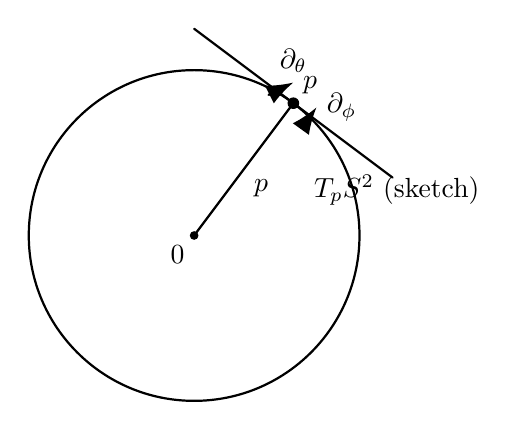
\begin{tikzpicture}[scale=1.05, line cap=round, line join=round]
		
		% Sphere as a circle (2D sketch)
		\draw[thick] (0,0) circle (2);
		
		% A point p on the sphere
		\coordinate (P) at (1.2,1.6); % roughly on the circle
		\fill (P) circle (2pt) node[above right] {$p$};
		
		% Radius vector
		\draw[thick] (0,0) -- (P) node[midway, below right] {$p$};
		
		% Tangent line at p (perpendicular to radius in this 2D sketch)
		% Tangent direction is perpendicular to OP; approximate slope
		\draw[thick] ($(P)+(-1.2,0.9)$) -- ($(P)+(1.2,-0.9)$);
		\node at ($(P)+(1.25,-1.05)$) {$T_pS^2$ (sketch)};
		
		% Small arrows indicating coordinate curves (conceptual)
		\draw[->, thick] ($(P)+(-0.3,0.1)$) -- ($(P)+(0.0,0.25)$) node[above] {$\partial_\theta$};
		\draw[->, thick] ($(P)+(0.1,-0.3)$) -- ($(P)+(0.28,-0.05)$) node[right] {$\partial_\phi$};
		
		% Center
		\fill (0,0) circle (1.5pt) node[below left] {$0$};
		
	\end{tikzpicture}
	\caption{Conceptual picture: a point $p\in S^2$, the radius vector, and the tangent plane $T_pS^2$ (drawn as a tangent line in 2D).}
\end{figure}

% ============================================================
% Tangent plane basis and “two coordinate directions” on S^2
% ============================================================

\subsection*{Tangent plane basis and ``two coordinate directions'' on $S^2$}

\paragraph{Tangent plane at $p$.}
For the unit sphere $S^2 \subset \mathbb{R}^3$ and a point $p \in S^2$,
the tangent plane at $p$ is
\[
T_p S^2 \;=\;\{\, v \in \mathbb{R}^3 \;:\; v \cdot p = 0 \,\}.
\]
This is a $2$-dimensional plane perpendicular to the radius vector $p$.
Geometrically, it is the plane through $p$ orthogonal to $p$.

\paragraph{How to get two coordinate directions in $T_pS^2$.}
There are two standard ways to obtain two independent tangent directions.

\medskip
\noindent\textbf{Method A: use a parametrization (spherical coordinates).}
Let
\[
F(\theta,\varphi)=\bigl(\sin\theta\cos\varphi,\ \sin\theta\sin\varphi,\ \cos\theta\bigr),
\qquad 0<\theta<\pi,\ \ 0<\varphi<2\pi,
\]
so that $p = F(\theta,\varphi)$. Then the two partial derivatives
\[
F_\theta(\theta,\varphi),\qquad F_\varphi(\theta,\varphi)
\]
are tangent vectors in $T_pS^2$ (and are linearly independent away from the poles).
They represent the coordinate directions of the $\theta$-curves and $\varphi$-curves.

To make them orthonormal, normalize:
\[
e_\theta \;=\;\frac{F_\theta}{\|F_\theta\|}, 
\qquad 
e_\varphi \;=\;\frac{F_\varphi}{\|F_\varphi\|}.
\]
On the unit sphere one has
\[
\|F_\theta\|=1,
\qquad 
\|F_\varphi\|=\sin\theta,
\]
so (away from the poles, where $\sin\theta\neq 0$)
\[
e_\theta = F_\theta,
\qquad
e_\varphi = \frac{1}{\sin\theta}\,F_\varphi.
\]
Then any tangent vector $v\in T_pS^2$ can be written uniquely as
\[
v \;=\; a\,e_\theta + b\,e_\varphi.
\]

\medskip
\noindent\textbf{Method B: use stereographic coordinates $(u,v)$.}
Stereographic projection
\[
\pi_N: S^2\setminus\{N\}\to \mathbb{R}^2
\]
gives coordinates $(u,v)$ on $S^2$ minus the north pole $N$.
In these coordinates, the natural coordinate directions at $p$ are the coordinate
vector fields
\[
\left.\frac{\partial}{\partial u}\right|_{p},
\qquad
\left.\frac{\partial}{\partial v}\right|_{p},
\]
which form a basis of $T_pS^2$. They need not be orthogonal in general, but you can
orthonormalize them (e.g.\ using Gram--Schmidt) to obtain two orthogonal directions
in the tangent plane.

\medskip
\noindent\textbf{Key idea:}
any chart (local coordinates) provides two tangent directions via its coordinate
vector fields. Orthogonality is an additional geometric choice, not automatic.



% ------------------------------------------------------------
% TikZ chart 2: stereographic projection sketch
% ------------------------------------------------------------
\begin{figure}[H]
	\centering
	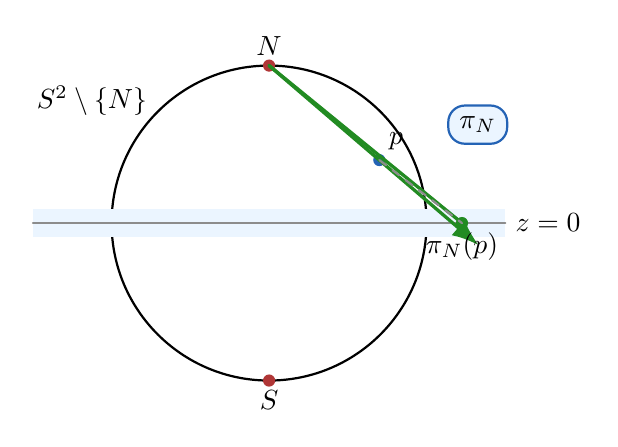
\begin{tikzpicture}[scale=1.0, line cap=round, line join=round]
		
		% ---- Colors ----
		\definecolor{blueA}{RGB}{36,99,181}
		\definecolor{redA}{RGB}{176,54,54}
		\definecolor{greenA}{RGB}{34,139,34}
		\definecolor{grayA}{RGB}{140,140,140}
		\definecolor{fillPlane}{RGB}{235,245,255}
		
		% ---- Sphere (2D sketch) ----
		\draw[thick] (0,0) circle (2);
		
		% ---- Equatorial plane z=0 (shown as a line) ----
		\fill[fillPlane] (-3,-0.18) rectangle (3,0.18); % a thin band to suggest the plane
		\draw[thick, draw=grayA] (-3,0) -- (3,0) node[right, black] {$z=0$};
		
		% ---- Poles ----
		\coordinate (N) at (0,2);
		\coordinate (S) at (0,-2);
		\fill[redA] (N) circle (2.2pt) node[above, black] {$N$};
		\fill[redA] (S) circle (2.2pt) node[below, black] {$S$};
		
		% ---- A point p on sphere (not north pole) ----
		\coordinate (P2) at (1.4,0.8);
		\fill[blueA] (P2) circle (2.2pt) node[above right, black] {$p$};
		
		% ---- Projection ray from N through p ----
		\draw[very thick, draw=greenA, ->] (N) -- ($(N)!1.9!(P2)$);
		
		% ---- Intersection point in the plane (chosen visually) ----
		\coordinate (Q) at (2.45,0);
		\fill[greenA] (Q) circle (2.2pt) node[below, black] {$\pi_N(p)$};
		
		% ---- Connect N to the projected point (same ray, emphasized) ----
		\draw[very thick, draw=greenA] (N) -- (Q);
		
		% ---- Optional helper: mark the line segment from p to Q as dashed (visual aid) ----
		\draw[thick, draw=grayA, dashed] (P2) -- (Q);
		
		% ---- Labels ----
		\node[draw=blueA, rounded corners=6pt, thick, inner sep=4pt, fill=fillPlane]
		at (2.65,1.25) {$\pi_N$};
		\node at (-2.25,1.55) {$S^2\setminus\{N\}$};
		
	\end{tikzpicture}
	\caption{Stereographic projection from the north pole $N$: the chart $\pi_N:S^2\setminus\{N\}\to\mathbb{R}^2$ (target plane $z=0$).}
\end{figure}

	
	% ============================================================
	% From a tangent basis (v1,v2) at p to (x,y)-coordinates
	% ============================================================
	
	\subsection*{From a tangent basis at $p$ to $(x,y)$-coordinates on the tangent plane}
	
	Suppose we have a point $p\in S^2$ and we choose two linearly independent tangent
	vectors
	\[
	v_1,\;v_2 \in T_pS^2.
	\]
	The key geometric point is:
	
	\medskip
	\noindent\textbf{The tangent plane is affine.}
	The tangent plane as a subset of $\mathbb{R}^3$ is the affine plane
	\[
	p + T_pS^2 \;=\;\{\,p+v : v\in T_pS^2\,\},
	\]
	which passes through $p$ (not through the origin in general).
	Its \emph{direction space} is the vector space $T_pS^2$.
	
	\medskip
	\noindent\textbf{Choosing an origin.}
	To introduce coordinates on the tangent plane, we pick an origin in that affine plane.
	The natural choice is the point $p$ itself. Then every point $q$ on the tangent plane
	can be written uniquely as
	\[
	q \;=\; p + x\,v_1 + y\,v_2,
	\]
	for some real numbers $(x,y)\in\mathbb{R}^2$.
	
	\paragraph{What exactly is being coordinated?}
	There are two closely related coordinate interpretations.
	
	\medskip
	\noindent\textbf{(1) Coordinates of a tangent vector.}
	Any tangent vector $v\in T_pS^2$ can be expressed as
	\[
	v \;=\; x\,v_1 + y\,v_2.
	\]
	Here $(x,y)$ are the coordinates of $v$ in the \emph{vector space} $T_pS^2$
	with respect to the basis $(v_1,v_2)$.
	
	\medskip
	\noindent\textbf{(2) Coordinates of a point on the tangent plane.}
	Any point $q$ on the affine plane $p+T_pS^2$ can be written as
	\[
	q \;=\; p + v \;=\; p + x\,v_1 + y\,v_2.
	\]
	The same pair $(x,y)$ now represents coordinates in the \emph{affine plane}
	using $p$ as the origin.
	
	\medskip
	\noindent\textbf{Important nuance: this does not give coordinates on the sphere itself.}
	The construction above gives coordinates on the \emph{tangent plane} (a flat plane).
	To map nearby tangent-plane coordinates $(x,y)$ onto the sphere $S^2$, one needs an
	additional map, for example:
	\begin{itemize}
		\item the exponential map $\exp_p: T_pS^2 \to S^2$ (geodesic motion on the surface), or
		\item a chart such as stereographic projection (sphere $\leftrightarrow$ a fixed plane,
		not necessarily the tangent plane at $p$).
	\end{itemize}
	
	\paragraph{Concrete example: the north pole.}
	Let
	\[
	p = N = (0,0,1).
	\]
	Then $T_pS^2$ consists of vectors orthogonal to $N$, i.e.\ vectors of the form $(a,b,0)$,
	and the tangent plane as an affine subset is the plane $z=1$.
	Choose the tangent basis
	\[
	v_1=(1,0,0),\qquad v_2=(0,1,0).
	\]
	Then any point $q$ in the tangent plane is
	\[
	q \;=\; (0,0,1) + x(1,0,0) + y(0,1,0)
	\;=\; (x,y,1).
	\]
	So in this case the coordinates are literally the usual $(x,y)$-coordinates on a plane.
	
	\paragraph{General point $p$.}
	For a general $p\in S^2$, choose any basis $v_1,v_2\in T_pS^2$ (often orthonormal).
	Then we have the identifications:
	\[
	\text{tangent vectors } v\in T_pS^2
	\;\longleftrightarrow\;
	(x,y)\in\mathbb{R}^2,
	\]
	and
	\[
	\text{points on the tangent plane } q\in p+T_pS^2
	\;\longleftrightarrow\;
	q = p + x v_1 + y v_2.
	\]
	
	% ============================================================
	% Orthonormal tangent basis on S^2 at p and (x,y)-coordinates
	% + mapping back to the sphere (normalization vs exponential map)
	% ============================================================
	
	\subsection*{Orthonormal coordinates on the tangent plane of $S^2$ at a point $p$}
	
	\paragraph{Setup.}
	Let
	\[
	S^2=\{x\in\mathbb{R}^3:\ \|x\|=1\}
	\]
	be the unit sphere and let $p\in S^2$.
	The tangent space at $p$ is the $2$-dimensional subspace
	\[
	T_pS^2=\{v\in\mathbb{R}^3:\ v\cdot p=0\}.
	\]
	The corresponding \emph{affine tangent plane} through $p$ is
	\[
	p+T_pS^2=\{p+v:\ v\in T_pS^2\}\subset\mathbb{R}^3.
	\]
	
	\subsection*{Constructing an orthonormal basis $(e_1,e_2)$ of $T_pS^2$}
	
	\paragraph{Step 1 (choose a helper vector not parallel to $p$).}
	Pick a vector $a\in\mathbb{R}^3$ such that $a$ is not parallel to $p$.
	A robust explicit choice is:
	\[
	a=
	\begin{cases}
		(0,0,1), & \text{if } |p\cdot(0,0,1)|<0.9,\\
		(0,1,0), & \text{otherwise}.
	\end{cases}
	\]
	This guarantees that $a$ is not too close to being parallel to $p$.
	
	\paragraph{Step 2 (project to the tangent plane).}
	Project $a$ orthogonally onto $T_pS^2$:
	\[
	u := a - (a\cdot p)\,p.
	\]
	Then $u\cdot p=0$, hence $u\in T_pS^2$, and $u\neq 0$ by the choice of $a$.
	
	\paragraph{Step 3 (normalize).}
	Define
	\[
	e_1 := \frac{u}{\|u\|}.
	\]
	Then $\|e_1\|=1$ and $e_1\in T_pS^2$.
	
	\paragraph{Step 4 (second orthonormal direction).}
	Set
	\[
	e_2 := p\times e_1.
	\]
	Then:
	\[
	e_2\cdot p=0\quad(\text{so }e_2\in T_pS^2),\qquad
	e_2\cdot e_1=0,\qquad
	\|e_2\|=1.
	\]
	Thus $(e_1,e_2)$ is an orthonormal basis of $T_pS^2$.
	
	\subsection*{$(x,y)$-coordinates on the tangent space and tangent plane}
	
	\paragraph{Coordinates of a tangent vector.}
	Every $v\in T_pS^2$ has a unique representation
	\[
	v = x\,e_1 + y\,e_2.
	\]
	The coefficients are obtained by dot products:
	\[
	x = v\cdot e_1,\qquad y = v\cdot e_2,
	\]
	because $(e_1,e_2)$ is orthonormal.
	
	\paragraph{Coordinates of a point on the affine tangent plane.}
	Every point $q\in p+T_pS^2$ can be written uniquely as
	\[
	q = p + v = p + x\,e_1 + y\,e_2.
	\]
	Hence $(x,y)$ are ordinary Euclidean coordinates on the tangent plane, with ``origin'' at the point $p$.
	
	\subsection*{Mapping tangent-plane coordinates back to the sphere}
	
	\paragraph{(A) Radial normalization map (simple projection).}
	Given $(x,y)$, form the tangent-plane point
	\[
	q(x,y)=p+x\,e_1+y\,e_2,
	\]
	and project radially back to the sphere:
	\[
	\Phi(x,y)=\frac{q(x,y)}{\|q(x,y)\|}=
	\frac{p+x\,e_1+y\,e_2}{\|p+x\,e_1+y\,e_2\|}.
	\]
	This gives a smooth local parametrization near $p$ for sufficiently small $\sqrt{x^2+y^2}$.
	
	\paragraph{(B) Exponential map (geodesic coordinates on $S^2$).}
	Let $v=x\,e_1+y\,e_2\in T_pS^2$ and set $r=\|v\|=\sqrt{x^2+y^2}$.
	The exponential map on the unit sphere is
	\[
	\exp_p(v)=
	\begin{cases}
		\cos r\, p + \sin r\, \dfrac{v}{r}, & r\neq 0,\\[0.8em]
		p, & r=0.
	\end{cases}
	\]
	This moves from $p$ along the great-circle geodesic in direction $v/\|v\|$ by spherical distance $r$.
	
	
	% ============================================================
	% Parallel transport on S^2 and the meaning of "standard coordinates"
	% ============================================================
	
	\subsection*{Parallel transport on $S^2$ and ``standard coordinates''}
	
	\paragraph{No single global smooth coordinate chart on $S^2$.}
	Although we often use \emph{spherical coordinates} $(\theta,\phi)$ on $S^2$,
	they are singular at the poles ($\phi$ is undefined at $\theta=0,\pi$).
	More generally, $S^2$ cannot be covered by a single smooth coordinate chart;
	one needs at least two charts (e.g.\ stereographic charts).
	Consequently, there is no globally defined, everywhere smooth intrinsic coordinate basis
	$(\partial_{u},\partial_{v})$ on all of $S^2$.
	
	\paragraph{What ``standard coordinates'' means for parallel transport.}
	Parallel transport compares tangent vectors at different points using the Levi--Civita connection.
	Given a smooth curve $\gamma:[0,T]\to S^2$ and an initial tangent vector $V(0)\in T_{\gamma(0)}S^2$,
	the \emph{parallel transported} vector field $V(t)\in T_{\gamma(t)}S^2$ is defined by the ODE
	\[
	\nabla_{\dot\gamma(t)}V(t)=0,
	\]
	where $\nabla$ is the Levi--Civita connection on $S^2$.
	
	If we choose an orthonormal basis $(e_1,e_2)$ of $T_{\gamma(0)}S^2$ and parallel transport each basis vector,
	we obtain an orthonormal frame along the curve,
	\[
	E_1(t),E_2(t)\in T_{\gamma(t)}S^2,\qquad \nabla_{\dot\gamma}E_i=0.
	\]
	This frame $(E_1(t),E_2(t))$ is the natural ``standard coordinate system'' along $\gamma$:
	every tangent vector $W(t)\in T_{\gamma(t)}S^2$ can be expressed uniquely as
	\[
	W(t)=x(t)\,E_1(t)+y(t)\,E_2(t),
	\]
	and the coefficients $(x(t),y(t))$ are consistent along the curve because the frame is parallel.
	
	\paragraph{A convenient global reference frame (not parallel transport).}
	Sometimes one wants a pointwise-defined reference basis without solving the parallel transport ODE.
	Fix a unit vector $k\in\mathbb{R}^3$ (e.g.\ $k=(0,0,1)$) and define for $p\in S^2$ (away from $p\parallel k$)
	\[
	e_1(p)=\frac{k-(k\cdot p)p}{\|k-(k\cdot p)p\|},\qquad e_2(p)=p\times e_1(p).
	\]
	Then $(e_1(p),e_2(p))$ is an orthonormal basis of $T_pS^2$ wherever it is defined.
	This provides a convenient ``gauge'' for coordinates on tangent planes, but it does \emph{not} coincide with
	parallel transport in general.
	
	\paragraph{Curvature and holonomy.}
	On $S^2$, parallel transport around a closed loop typically returns a vector rotated by a nonzero angle.
	This phenomenon (holonomy) reflects the nonzero Gaussian curvature of the sphere and is not removable by choosing
	different coordinates.
	
	% ============================================================
	% Parallel transport along a curve on S^2 and orthonormal bases in tangent planes
	% ============================================================
	
	\subsection*{Parallel transport along a curve on $S^2$ and orthonormal bases of tangent planes}
	
	\paragraph{Tangent bundle along a curve (a rank-2 vector bundle).}
	Let $\gamma:[0,T]\to S^2$ be a smooth curve.
	The family of tangent planes $\{T_{\gamma(t)}S^2\}_{t\in[0,T]}$ forms the pullback bundle
	\[
	\gamma^*(TS^2)\to [0,T],
	\]
	a rank-$2$ vector bundle whose fiber at $t$ is $T_{\gamma(t)}S^2$.
	
	\paragraph{(1) Orthonormal bases via parallel transport.}
	Fix an orthonormal basis $(E_1(0),E_2(0))$ of $T_{\gamma(0)}S^2$.
	Define vector fields $E_i(t)\in T_{\gamma(t)}S^2$ by the parallel transport equations
	\[
	\nabla_{\dot\gamma(t)}E_i(t)=0,\qquad E_i(0)\ \text{given},\quad i=1,2,
	\]
	where $\nabla$ is the Levi--Civita connection on $S^2$.
	
	Because $\nabla$ is metric-compatible,
	\[
	\frac{d}{dt}\langle E_i(t),E_j(t)\rangle
	=
	\langle \nabla_{\dot\gamma}E_i, E_j\rangle + \langle E_i,\nabla_{\dot\gamma}E_j\rangle = 0.
	\]
	Hence orthonormality is preserved:
	if $(E_1(0),E_2(0))$ is orthonormal at $t=0$, then $(E_1(t),E_2(t))$ is orthonormal for all $t$.
	
	\paragraph{(2) Explicit parallel transport ODE in $\mathbb{R}^3$ for the unit sphere.}
	View $S^2\subset\mathbb{R}^3$ with the induced metric and write $p(t)=\gamma(t)$.
	Then
	\[
	T_{p(t)}S^2=\{V\in\mathbb{R}^3:\ V\cdot p(t)=0\}.
	\]
	A vector field $V(t)\in\mathbb{R}^3$ along $\gamma$ is parallel on $S^2$ iff its Euclidean derivative
	has no tangential component, i.e.
	\[
	\mathrm{proj}_{T_{p(t)}S^2}\big(\dot V(t)\big)=0.
	\]
	For the unit sphere the normal direction at $p(t)$ is $p(t)$ itself, so this is equivalent to
	$\dot V(t)=\lambda(t)\,p(t)$ for some scalar $\lambda(t)$.
	Differentiating the constraint $V(t)\cdot p(t)=0$ gives
	\[
	0=\frac{d}{dt}\big(V\cdot p\big)=\dot V\cdot p + V\cdot \dot p
	= \lambda(t)\, (p\cdot p) + V\cdot \dot p
	= \lambda(t) + V\cdot \dot\gamma(t),
	\]
	hence $\lambda(t)=-(V\cdot \dot\gamma)$ and therefore the parallel transport equation becomes
	\[
	\boxed{\ \dot V(t)=-(V(t)\cdot \dot\gamma(t))\,\gamma(t)\ }.
	\]
	Solving this ODE with initial data $V(0)\in T_{\gamma(0)}S^2$ yields the parallel-transported field.
	Applying it to two initial orthonormal vectors produces an orthonormal basis in each $T_{\gamma(t)}S^2$.
	
	\paragraph{(3) A pointwise orthonormal frame (a gauge), not parallel transport.}
	Sometimes one only needs a convenient orthonormal basis in each $T_pS^2$ without requiring parallel transport.
	Fix a unit vector $k\in\mathbb{R}^3$ (e.g.\ $k=(0,0,1)$). For $p\in S^2$ with $p\not\parallel k$ define
	\[
	e_1(p)=\frac{k-(k\cdot p)p}{\|k-(k\cdot p)p\|},\qquad e_2(p)=p\times e_1(p).
	\]
	Then $(e_1(p),e_2(p))$ is an orthonormal basis of $T_pS^2$ wherever it is defined.
	Near points where $p\parallel k$ one switches to a different reference vector $k$.
	This provides a global frame by patching charts, but in general it does \emph{not} coincide with parallel transport.
	
	% ============================================================
	% What [0,T] means in gamma:[0,T]->S^2 and in the pullback bundle gamma^*(TS^2)->[0,T]
	% ============================================================
	
	\subsection*{What does the interval $[0,T]$ mean in $\gamma^*(TS^2)\to[0,T]$?}
	
	Let
	\[
	\gamma:[0,T]\to S^2
	\]
	be a smooth curve on the sphere. Here $[0,T]$ is simply the \emph{parameter interval} (often interpreted as time).
	For each parameter value $t\in[0,T]$, the point $\gamma(t)\in S^2$ is the position of the curve at time $t$.
	
	\paragraph{The pullback tangent bundle along the curve.}
	The tangent bundle $TS^2\to S^2$ assigns to each point $p\in S^2$ its tangent plane $T_pS^2$.
	Pulling this bundle back by $\gamma$ produces a rank-$2$ vector bundle over the interval $[0,T]$:
	\[
	\gamma^*(TS^2)\longrightarrow [0,T].
	\]
	Concretely, the total space of the pullback bundle is
	\[
	\gamma^*(TS^2)=\{(t,v):\ t\in[0,T],\ v\in T_{\gamma(t)}S^2\},
	\]
	and the projection map is
	\[
	\pi(t,v)=t.
	\]
	Thus the fiber over $t$ is precisely the tangent space at the point $\gamma(t)$:
	\[
	\big(\gamma^*(TS^2)\big)_t \;=\; T_{\gamma(t)}S^2.
	\]
	
	\paragraph{Interpretation.}
	The bundle $\gamma^*(TS^2)\to[0,T]$ is a convenient way to package \emph{all tangent planes along the curve}
	into a single vector bundle whose base is the parameter interval.
	A section of this bundle is the same thing as a tangent vector field along the curve:
	\[
	V:[0,T]\to TS^2,\qquad V(t)\in T_{\gamma(t)}S^2.
	\]
	
		% ============================================================
	% Concrete computations on S^2: tangent planes, orthonormal bases, coordinates
	% ============================================================
	
	\subsection*{Concrete computations on $S^2$: tangent planes, orthonormal bases, and coordinates}
	
	\paragraph{General fact (unit sphere).}
	For $p\in S^2\subset\mathbb{R}^3$ with $\|p\|=1$, the tangent space is
	\[
	T_pS^2=\{v\in\mathbb{R}^3:\ v\cdot p=0\}.
	\]
	
	% ------------------------------------------------------------
	% Example 1: Equator
	% ------------------------------------------------------------
	\subsubsection*{Example 1: the equator $\gamma(t)=(\cos t,\sin t,0)$}
	
	Let
	\[
	\gamma(t)=(\cos t,\ \sin t,\ 0),\qquad t\in[0,2\pi].
	\]
	Then $\|\gamma(t)\|=1$, so $\gamma(t)\in S^2$.
	
	\paragraph{Tangent plane.}
	At $p=\gamma(t)$,
	\[
	T_{\gamma(t)}S^2=\{v\in\mathbb{R}^3:\ v\cdot \gamma(t)=0\}.
	\]
	
	\paragraph{Orthonormal basis of $T_{\gamma(t)}S^2$.}
	Differentiate:
	\[
	\gamma'(t)=(-\sin t,\ \cos t,\ 0),\qquad \|\gamma'(t)\|=1.
	\]
	Thus we may take
	\[
	e_1(t)=\gamma'(t)=(-\sin t,\ \cos t,\ 0).
	\]
	Also set
	\[
	e_2(t)=(0,0,1).
	\]
	Then
	\[
	e_2(t)\cdot \gamma(t)=0,\quad e_1(t)\cdot e_2(t)=0,\quad \|e_1(t)\|=\|e_2(t)\|=1,
	\]
	so $(e_1(t),e_2(t))$ is an orthonormal basis of $T_{\gamma(t)}S^2$.
	
	\paragraph{Coordinates of a tangent vector.}
	Given coordinates $(x,y)\in\mathbb{R}^2$, define
	\[
	v(t)=x\,e_1(t)+y\,e_2(t).
	\]
	For example, if $(x,y)=(2,-\tfrac12)$ then
	\[
	v(t)=2e_1(t)-\tfrac12 e_2(t)=(-2\sin t,\ 2\cos t,\ -\tfrac12).
	\]
	It is tangent because
	\[
	v(t)\cdot \gamma(t)=(-2\sin t)\cos t + (2\cos t)\sin t + (-\tfrac12)\cdot 0 = 0.
	\]
	Conversely, the coordinates are recovered by dot products:
	\[
	x=v(t)\cdot e_1(t),\qquad y=v(t)\cdot e_2(t),
	\]
	since $(e_1,e_2)$ is orthonormal.
	
	% ------------------------------------------------------------
	% Example 2: Latitude
	% ------------------------------------------------------------
	\subsubsection*{Example 2: a latitude circle $\gamma(t)=(r\cos t,r\sin t,z_0)$}
	
	Fix $z_0\in(-1,1)$ and set $r=\sqrt{1-z_0^2}$. Define
	\[
	\gamma(t)=(r\cos t,\ r\sin t,\ z_0),\qquad t\in[0,2\pi].
	\]
	Then $\|\gamma(t)\|^2=r^2+z_0^2=1$, so $\gamma(t)\in S^2$.
	
	\paragraph{Tangent plane.}
	At $p=\gamma(t)$,
	\[
	T_{\gamma(t)}S^2=\{v\in\mathbb{R}^3:\ v\cdot \gamma(t)=0\}.
	\]
	
	\paragraph{Orthonormal basis of $T_{\gamma(t)}S^2$.}
	Differentiate:
	\[
	\gamma'(t)=(-r\sin t,\ r\cos t,\ 0),\qquad \|\gamma'(t)\|=r.
	\]
	Hence the unit tangent direction is
	\[
	e_1(t)=\frac{\gamma'(t)}{\|\gamma'(t)\|}=(-\sin t,\ \cos t,\ 0).
	\]
	Define the second basis vector by
	\[
	e_2(t)=\gamma(t)\times e_1(t).
	\]
	Compute:
	\[
	\gamma(t)\times e_1(t)
	=(r\cos t,\ r\sin t,\ z_0)\times(-\sin t,\ \cos t,\ 0)
	=(-z_0\cos t,\ -z_0\sin t,\ r).
	\]
	Its norm is
	\[
	\|e_2(t)\|=\sqrt{z_0^2(\cos^2 t+\sin^2 t)+r^2}=\sqrt{z_0^2+r^2}=1,
	\]
	so it is already unit. Therefore
	\[
	e_2(t)=(-z_0\cos t,\ -z_0\sin t,\ r),
	\]
	and $(e_1(t),e_2(t))$ is an orthonormal basis of $T_{\gamma(t)}S^2$.
	
	\paragraph{Coordinates of a tangent vector.}
	Given $(x,y)\in\mathbb{R}^2$, define
	\[
	v(t)=x\,e_1(t)+y\,e_2(t).
	\]
	For example, with $(x,y)=(1,3)$ we get
	\[
	v(t)=e_1(t)+3e_2(t)
	=(-\sin t-3z_0\cos t,\ \cos t-3z_0\sin t,\ 3r).
	\]
	Again, coordinates recover by dot products:
	\[
	x=v(t)\cdot e_1(t),\qquad y=v(t)\cdot e_2(t).
	\]
	
	% ============================================================
	% Practical computation on a general surface Σ ⊂ R^3:
	% parallel transport ODE in R^3 using the unit normal n(t)
	% ============================================================
	
	\subsection*{Practical computation on a general surface $\Sigma \subset \mathbb{R}^3$: an explicit ODE in $\mathbb{R}^3$}
	
	Let $\Sigma \subset \mathbb{R}^3$ be a smooth oriented surface with unit normal field $n$.
	Let $\gamma:[0,T]\to \Sigma$ be a smooth curve, and write
	\[
	n(t):=n(\gamma(t)) \in S^2.
	\]
	A vector field $V(t)\in\mathbb{R}^3$ along $\gamma$ is a \emph{tangent vector field} iff
	\[
	V(t)\in T_{\gamma(t)}\Sigma
	\quad\Longleftrightarrow\quad
	V(t)\cdot n(t)=0 \ \ \text{for all }t.
	\]
	
	\paragraph{Levi--Civita connection as tangential projection.}
	For a surface embedded in $\mathbb{R}^3$, the Levi--Civita covariant derivative along $\gamma$ is given by
	\[
	\nabla_{\dot\gamma(t)}V(t) \;=\; \mathrm{proj}_{T_{\gamma(t)}\Sigma}\big(\dot V(t)\big),
	\]
	i.e.\ the tangential component of the ordinary derivative in $\mathbb{R}^3$.
	
	\paragraph{Parallel transport condition.}
	The vector field $V(t)$ is \emph{parallel along $\gamma$} on the surface iff
	\[
	\nabla_{\dot\gamma(t)}V(t)=0
	\quad\Longleftrightarrow\quad
	\mathrm{proj}_{T_{\gamma(t)}\Sigma}\big(\dot V(t)\big)=0.
	\]
	Equivalently, $\dot V(t)$ has no tangential component, so it must be purely normal:
	\[
	\dot V(t)=\lambda(t)\,n(t)
	\]
	for some scalar function $\lambda(t)$.
	
	\paragraph{Determine $\lambda(t)$ from the tangency constraint.}
	Differentiate the constraint $V(t)\cdot n(t)=0$:
	\[
	0=\frac{d}{dt}\big(V\cdot n\big)=\dot V\cdot n + V\cdot \dot n.
	\]
	Using $\dot V=\lambda n$ and $n\cdot n=1$ gives
	\[
	0=\lambda(t) + V(t)\cdot \dot n(t)
	\qquad\Longrightarrow\qquad
	\lambda(t)=-(V(t)\cdot \dot n(t)).
	\]
	
	\paragraph{Parallel transport ODE in $\mathbb{R}^3$.}
	Substituting back, the parallel transport equation becomes
	\[
	\boxed{\ \dot V(t)=-(V(t)\cdot \dot n(t))\,n(t)\ }
	\]
	together with the constraint $V(0)\cdot n(0)=0$ (so $V(0)\in T_{\gamma(0)}\Sigma$).
	
	\paragraph{Remarks.}
	\begin{itemize}
		\item On the unit sphere $\Sigma=S^2$, one has $n(t)=\gamma(t)$, hence $\dot n(t)=\dot\gamma(t)$, and the formula reduces to
		\[
		\dot V(t)=-(V(t)\cdot \dot\gamma(t))\,\gamma(t),
		\]
		exactly as before.
		\item To obtain an orthonormal basis of each tangent plane along $\gamma$, choose two orthonormal initial vectors
		$E_1(0),E_2(0)\in T_{\gamma(0)}\Sigma$ and solve the ODE for each $E_i(t)$.
		Metric-compatibility implies orthonormality is preserved.
	\end{itemize}
	
	% ------------------------------------------------------------
	% Optional: implicit surface specialization (if Σ is given by f=0)
	% ------------------------------------------------------------
	
	\subsubsection*{Optional specialization: $\Sigma=\{f=0\}$ is an implicit surface}
	
	Assume $\Sigma$ is given as a regular level set
	\[
	\Sigma=\{x\in\mathbb{R}^3:\ f(x)=0\},\qquad \nabla f\neq 0\ \text{on }\Sigma.
	\]
	A unit normal is
	\[
	n(x)=\frac{\nabla f(x)}{\|\nabla f(x)\|}.
	\]
	Along $\gamma(t)$ we have $n(t)=n(\gamma(t))$ and
	\[
	\dot n(t)=Dn(\gamma(t))\,\dot\gamma(t),
	\]
	so the same ODE becomes
	\[
	\dot V(t)=-(V(t)\cdot Dn(\gamma(t))\,\dot\gamma(t))\,n(\gamma(t)).
	\]
	

% ============================================================
% Parallel transport on S^2 along the equator: explicit computation
% ============================================================

\subsection*{Parallel transport on $S^2$ along the equator (explicit computation)}

Let
\[
\gamma(t)=(\cos t,\ \sin t,\ 0),\qquad t\in[0,2\pi].
\]
This is a unit-speed great circle on $S^2$, so the unit normal is $n(t)=\gamma(t)$.
The parallel transport equation in $\mathbb{R}^3$ is
\[
\dot V(t)=-(V(t)\cdot \dot\gamma(t))\,\gamma(t),
\qquad V(t)\cdot \gamma(t)=0.
\]

\paragraph{An orthonormal tangent frame along the equator.}
Compute
\[
\dot\gamma(t)=(-\sin t,\ \cos t,\ 0),\qquad \|\dot\gamma(t)\|=1.
\]
Define
\[
e_1(t)=\dot\gamma(t)=(-\sin t,\ \cos t,\ 0),\qquad e_2=(0,0,1).
\]
Then $e_1(t)\cdot \gamma(t)=0$ and $e_2\cdot \gamma(t)=0$, so both are tangent, and they are orthonormal.

\paragraph{Transport of $e_2$.}
Let $V(t)=e_2=(0,0,1)$. Then $\dot V(t)=0$, and
\[
V(t)\cdot \dot\gamma(t)=(0,0,1)\cdot(-\sin t,\cos t,0)=0.
\]
Hence the ODE gives $\dot V(t)=-(0)\gamma(t)=0$, so $e_2$ is parallel along $\gamma$.

\paragraph{Transport of $e_1(t)=\dot\gamma(t)$.}
Let $V(t)=e_1(t)=\dot\gamma(t)$. Then
\[
\dot V(t)=\ddot\gamma(t)=(-\cos t,\ -\sin t,\ 0)=-\gamma(t),
\]
and also
\[
V(t)\cdot \dot\gamma(t)=\dot\gamma(t)\cdot \dot\gamma(t)=1.
\]
Thus the ODE predicts
\[
\dot V(t)=-(1)\gamma(t)=-\gamma(t),
\]
which matches $\ddot\gamma(t)$. Therefore $e_1(t)$ is also parallel along $\gamma$.

\paragraph{Conclusion.}
If $(E_1(0),E_2(0))=(e_1(0),e_2)$ is an orthonormal basis of $T_{\gamma(0)}S^2$, then its parallel transport is
\[
E_1(t)=e_1(t)=(-\sin t,\cos t,0),\qquad E_2(t)=e_2=(0,0,1).
\]
After one loop, $E_i(2\pi)=E_i(0)$, i.e.\ there is no net rotation for this great circle.


% ============================================================
% Two curves between (lat,lon)=(0,0) and (10,10) on S^2:
% (1) Great-circle (geodesic)
% (2) Lat--lon linear path  (phi(t)=kt, lambda(t)=kt)
% Tangent planes, orthonormal frames, and parallel transport
% ============================================================

\subsection*{Two paths on $S^2$ between $(\varphi,\lambda)=(0^\circ,0^\circ)$ and $(10^\circ,10^\circ)$}

\paragraph{Lat--lon to $S^2\subset\mathbb{R}^3$.}
Using latitude $\varphi$ and longitude $\lambda$ (in radians inside trig),
\[
p(\varphi,\lambda)=\big(\cos\varphi\cos\lambda,\ \cos\varphi\sin\lambda,\ \sin\varphi\big)\in S^2.
\]
Hence
\[
A=p(0,0)=(1,0,0),
\]
and
\[
B=p(10^\circ,10^\circ)
=\big(\cos 10^\circ\cos 10^\circ,\ \cos 10^\circ\sin 10^\circ,\ \sin 10^\circ\big).
\]

\paragraph{Parallel transport ODE on the unit sphere.}
For a smooth curve $\gamma(t)\in S^2$ and a tangent field $V(t)\in T_{\gamma(t)}S^2$,
parallel transport is equivalent to the explicit $\mathbb{R}^3$ ODE
\[
\boxed{\ \dot V(t)=-(V(t)\cdot \dot\gamma(t))\,\gamma(t)\ },\qquad V(t)\cdot \gamma(t)=0.
\]

% ------------------------------------------------------------
% (1) Great-circle (geodesic) between A and B
% ------------------------------------------------------------
\subsubsection*{(1) Great-circle (geodesic) between $A$ and $B$}

Let
\[
\alpha=\arccos(A\cdot B)\in(0,\pi)
\]
be the central angle between $A$ and $B$.
Define the unit tangent direction at $A$ pointing toward $B$ by
\[
U=\frac{B-(A\cdot B)A}{\|B-(A\cdot B)A\|}\in T_A S^2.
\]
Then the great-circle arc from $A$ to $B$ is
\[
\boxed{\ \gamma_{\mathrm{gc}}(t)=\cos t\,A+\sin t\,U,\qquad t\in[0,\alpha]\ }.
\]
One checks $\gamma_{\mathrm{gc}}(0)=A$ and $\gamma_{\mathrm{gc}}(\alpha)=B$, and $\|\dot\gamma_{\mathrm{gc}}(t)\|=1$.

\paragraph{A natural orthonormal tangent frame along the great circle.}
Define
\[
E_1(t)=\dot\gamma_{\mathrm{gc}}(t)=-\sin t\,A+\cos t\,U,
\]
and the constant vector
\[
N:=A\times U.
\]
Then $N\cdot \gamma_{\mathrm{gc}}(t)=0$ for all $t$, so $N\in T_{\gamma_{\mathrm{gc}}(t)}S^2$ everywhere.
Moreover, $\|E_1(t)\|=\|N\|=1$ and $E_1(t)\cdot N=0$, hence
\[
(E_1(t),E_2(t))\ \text{with}\ E_2(t):=N
\]
is an orthonormal basis of $T_{\gamma_{\mathrm{gc}}(t)}S^2$ for all $t$.

\paragraph{Parallel transport along the great circle.}
Along a great circle, both $E_1(t)=\dot\gamma_{\mathrm{gc}}(t)$ and the constant $N$ satisfy the parallel transport ODE,
so any field with constant coefficients in this frame is parallel.
If
\[
V(0)=a_0\,E_1(0)+b_0\,E_2(0)=a_0\,U+b_0\,N,
\]
then the parallel-transported vector field is explicitly
\[
\boxed{\ V(t)=a_0\,E_1(t)+b_0\,N,\qquad t\in[0,\alpha].\ }
\]
In particular, $V(\alpha)$ is the transported vector in $T_BS^2$.

% ------------------------------------------------------------
% (2) Lat--lon linear path phi(t)=kt, lambda(t)=kt
% ------------------------------------------------------------
\subsubsection*{(2) Lat--lon linear path: $\varphi(t)=kt,\ \lambda(t)=kt$}

Let $t\in[0,1]$ and set
\[
k=10^\circ=\frac{\pi}{18}\ \text{(radians)}.
\]
Define the curve
\[
\boxed{\ \gamma_{\mathrm{ll}}(t)=p(\varphi(t),\lambda(t))=
	\big(\cos(kt)\cos(kt),\ \cos(kt)\sin(kt),\ \sin(kt)\big),\qquad t\in[0,1].\ }
\]
Then $\gamma_{\mathrm{ll}}(0)=A$ and $\gamma_{\mathrm{ll}}(1)=B$.

\paragraph{Tangent vectors from the coordinate derivatives.}
The coordinate partial derivatives of $p(\varphi,\lambda)$ are
\[
\partial_\varphi p=(-\sin\varphi\cos\lambda,\ -\sin\varphi\sin\lambda,\ \cos\varphi),
\]
\[
\partial_\lambda p=(-\cos\varphi\sin\lambda,\ \cos\varphi\cos\lambda,\ 0).
\]
Since $\varphi'(t)=k$ and $\lambda'(t)=k$, the velocity is
\[
\dot\gamma_{\mathrm{ll}}(t)=k\,\partial_\varphi p(\varphi,\lambda)+k\,\partial_\lambda p(\varphi,\lambda),
\qquad \varphi=\lambda=kt.
\]

\paragraph{An orthonormal basis of each tangent plane along $\gamma_{\mathrm{ll}}$.}
Define the unit tangent direction
\[
e_1(t)=\frac{\dot\gamma_{\mathrm{ll}}(t)}{\|\dot\gamma_{\mathrm{ll}}(t)\|},
\]
and a second unit tangent direction by
\[
e_2(t)=\frac{\gamma_{\mathrm{ll}}(t)\times e_1(t)}{\|\gamma_{\mathrm{ll}}(t)\times e_1(t)\|}.
\]
Then $(e_1(t),e_2(t))$ is an orthonormal basis of $T_{\gamma_{\mathrm{ll}}(t)}S^2$ for each $t$.

\paragraph{Concrete basis at the start.}
At $t=0$, $\gamma_{\mathrm{ll}}(0)=(1,0,0)$ and
\[
\dot\gamma_{\mathrm{ll}}(0)=k(0,1,1),
\]
so
\[
e_1(0)=\frac{1}{\sqrt2}(0,1,1),
\qquad
e_2(0)=\gamma_{\mathrm{ll}}(0)\times e_1(0)=\frac{1}{\sqrt2}(0,-1,1).
\]

\paragraph{Parallel transport along the lat--lon path.}
Given an initial tangent vector $V(0)\in T_{A}S^2$ (equivalently $V(0)\cdot A=0$),
the parallel-transported vector field along $\gamma_{\mathrm{ll}}$ is the solution of
\[
\boxed{\ \dot V(t)=-(V(t)\cdot \dot\gamma_{\mathrm{ll}}(t))\,\gamma_{\mathrm{ll}}(t),\qquad
	V(0)\cdot \gamma_{\mathrm{ll}}(0)=0.\ }
\]
This generally has no simple closed form and is typically solved numerically.

\paragraph{Fresh frames vs.\ transported frames.}
The basis $(e_1(t),e_2(t))$ constructed above is a \emph{fresh} orthonormal frame at each tangent plane.
If one needs a frame that varies ``as little as possible'' along the curve (to compare coordinates consistently),
one instead parallel-transports an initial orthonormal basis $(E_1(0),E_2(0))$ by solving the ODE for each $E_i(t)$.

	
	\subsection*{Problem 5: de Rham cohomology of spheres via $U_\pm$}
	
	\noindent \textbf{Problem statement.}
	Let
	\[
	U_\pm = S^n\setminus\{(0,\dots,0,\pm 1)\}.
	\]
	(a) Show that $H^1_{\mathrm{dR}}(S^n)=0$ for $n\ge 2$ by taking a closed $1$-form $\alpha$ and considering
	its restrictions to $U_\pm$.
	(b) For $n\ge 1$ prove by induction that
	\[
	H^r_{\mathrm{dR}}(S^n)\cong
	\begin{cases}
		\mathbb{R}, & r=0 \text{ or } r=n,\\
		0, & \text{otherwise}.
	\end{cases}
	\]
	Hint: $U_+\cap U_-$ is homotopy equivalent to $S^{n-1}$.
	
	\medskip
	\noindent \textbf{Solution.}
	Each $U_\pm$ is diffeomorphic to $\mathbb{R}^n$ (stereographic projection), hence
	$H^k_{\mathrm{dR}}(U_\pm)=0$ for $k\ge 1$.
	Moreover $U_+\cap U_-=S^n\setminus\{\text{north,south}\}$ deformation retracts onto the equator $S^{n-1}$, so
	\[
	H^k_{\mathrm{dR}}(U_+\cap U_-)\cong H^k_{\mathrm{dR}}(S^{n-1}).
	\]
	
	\smallskip
	\textit{(a)} Let $\alpha$ be a closed $1$-form on $S^n$. Since $H^1(U_\pm)=0$,
	there exist smooth functions $f_\pm$ on $U_\pm$ such that
	\[
	\alpha|_{U_\pm}=df_\pm.
	\]
	On the overlap $U_+\cap U_-$ we have
	\[
	d(f_+-f_-)=df_+-df_-=\alpha-\alpha=0,
	\]
	so $f_+-f_-$ is locally constant. For $n\ge 2$ the overlap is connected (it is homotopy equivalent to $S^{n-1}$),
	so $f_+-f_-=c$ is a constant. Define a global function $f$ by
	\[
	f=
	\begin{cases}
		f_+ & \text{on }U_+,\\
		f_-+c & \text{on }U_-.
	\end{cases}
	\]
	This is well-defined and smooth, and $df=\alpha$. Hence $\alpha$ is exact and $H^1_{\mathrm{dR}}(S^n)=0$.
	
	\smallskip
	\textit{(b)} Apply the Mayer--Vietoris long exact sequence to $S^n=U_+\cup U_-$:
	\[
	\cdots \to H^{r-1}(U_+\cap U_-)\xrightarrow{\delta}
	H^r(S^n)\to H^r(U_+)\oplus H^r(U_-)\to H^r(U_+\cap U_-)\to \cdots
	\]
	For $r\ge 1$, $H^r(U_\pm)=0$, hence
	\[
	H^r(S^n)\cong H^{r-1}(U_+\cap U_-)\cong H^{r-1}(S^{n-1})
	\qquad (1\le r\le n-1).
	\]
	With the base case $n=1$ (where $H^0(S^1)\cong\mathbb{R}$ and $H^1(S^1)\cong\mathbb{R}$),
	this recursion implies $H^r(S^n)=0$ for $1\le r\le n-1$.
	Also $H^0(S^n)\cong\mathbb{R}$ since $S^n$ is connected, and $H^n(S^n)\cong\mathbb{R}$
	(e.g.\ because $S^n$ is a connected closed oriented $n$-manifold, so the top de Rham cohomology is one-dimensional).
	Therefore
	\[
	H^r_{\mathrm{dR}}(S^n)\cong
	\begin{cases}
		\mathbb{R}, & r=0 \text{ or } r=n,\\
		0, & \text{otherwise}.
	\end{cases}
	\]
	
	% ============================================================
	% Theory: Problem 5 (de Rham cohomology of spheres via U_±)
	% ============================================================
	

\subsection*{Theory for Problem 5: Computing $H^*_{\mathrm{dR}}(S^n)$ via $U_\pm$}

\paragraph{Contractible charts and the Poincar\'e lemma.}
Let
\[
U_\pm := S^n\setminus\{(0,\dots,0,\pm 1)\}.
\]
By stereographic projection, each $U_\pm$ is diffeomorphic to $\mathbb{R}^n$, hence contractible.
Therefore, by the Poincar\'e lemma,
\[
H^k_{\mathrm{dR}}(U_\pm)=0 \quad (k\ge 1),
\qquad
H^0_{\mathrm{dR}}(U_\pm)\cong \mathbb{R}.
\]

\paragraph{The overlap deformation retracts to the equator.}
The intersection
\[
U_+\cap U_- = S^n\setminus\{\text{north pole, south pole}\}
\]
admits a deformation retraction onto the equator $S^{n-1}$ (push along meridians).
Hence
\[
H^k_{\mathrm{dR}}(U_+\cap U_-)\cong H^k_{\mathrm{dR}}(S^{n-1}).
\]

\paragraph{Mayer--Vietoris long exact sequence (de Rham).}
For an open cover $M=U\cup V$ there is a long exact sequence
\[
\cdots \to H^{r-1}(U\cap V)\xrightarrow{\delta} H^r(M)
\to H^r(U)\oplus H^r(V)\to H^r(U\cap V)\to \cdots
\]
relating the cohomology of $M$ to that of $U$, $V$, and $U\cap V$.

\paragraph{How the sphere computation follows.}
Applying Mayer--Vietoris to $S^n=U_+\cup U_-$, the vanishing $H^r(U_\pm)=0$ for $r\ge 1$
forces the recursion
\[
H^r(S^n)\cong H^{r-1}(U_+\cap U_-)\cong H^{r-1}(S^{n-1})
\qquad (1\le r\le n-1).
\]
This ``degree shift'' yields inductively that $H^r(S^n)=0$ for $0<r<n$.
Also $H^0(S^n)\cong\mathbb{R}$ since $S^n$ is connected, and $H^n(S^n)\cong\mathbb{R}$
(the top de Rham class, e.g.\ represented by a volume form on an oriented sphere).

\paragraph{Elementary gluing idea for $H^1(S^n)=0$ when $n\ge 2$.}
If $\alpha$ is a closed $1$-form on $S^n$, then on each $U_\pm\simeq\mathbb{R}^n$ there exist
functions $f_\pm$ with $\alpha|_{U_\pm}=df_\pm$.
On $U_+\cap U_-$ one has $d(f_+-f_-)=0$, so $f_+-f_-$ is locally constant.
For $n\ge 2$, the overlap is connected (it retracts to $S^{n-1}$), hence $f_+-f_-$ is constant,
and one can glue $f_\pm$ to a global function $f$ with $\alpha=df$.


	\begin{figure}[H]
		\centering
		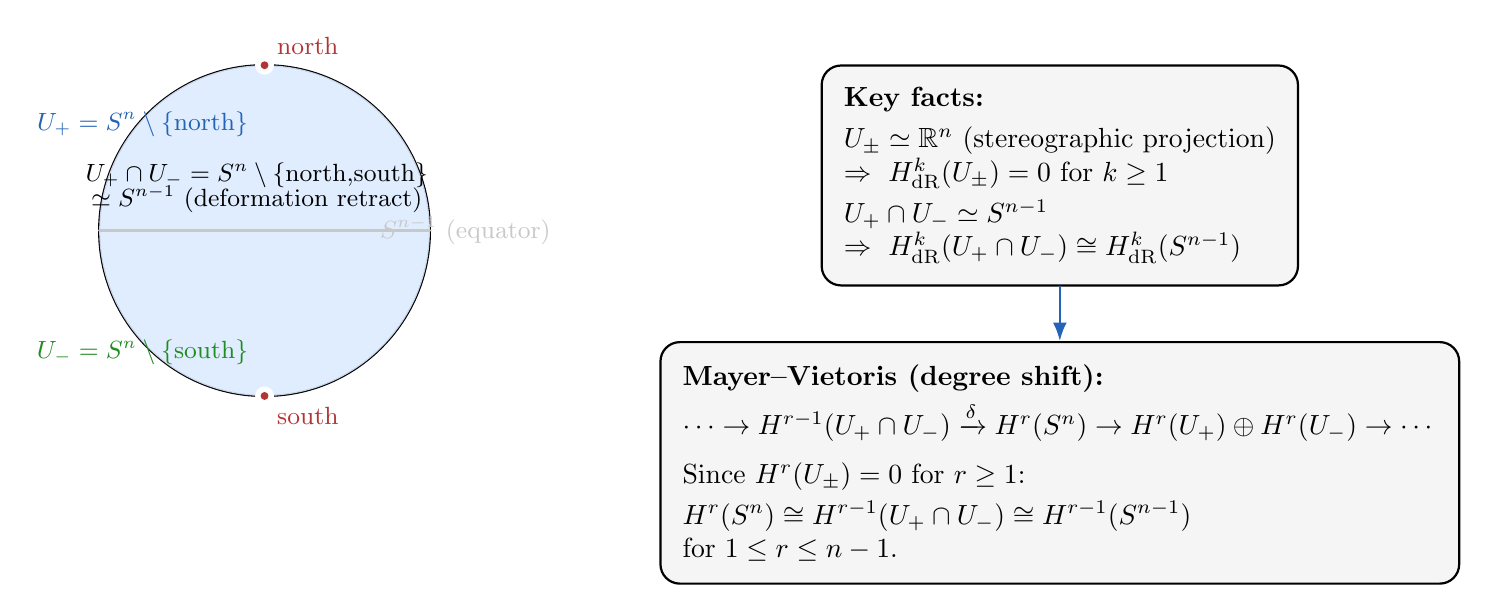
\begin{tikzpicture}[>=Latex, line cap=round, line join=round]
			
			\definecolor{blueA}{RGB}{36,99,181}
			\definecolor{greenA}{RGB}{34,139,34}
			\definecolor{redA}{RGB}{176,54,54}
			\definecolor{grayB}{RGB}{245,245,245}
			\definecolor{fillU}{RGB}{220,235,255}
			\definecolor{fillV}{RGB}{235,255,230}
			\definecolor{eqA}{RGB}{200,200,200}
			
			\tikzset{
				box/.style={rounded corners=7pt, draw=black, thick, fill=grayB, inner sep=8pt, align=left},
				arrowB/.style={->, thick, draw=blueA},
				arrowG/.style={->, thick, draw=greenA},
				arrowR/.style={->, thick, draw=redA},
				lab/.style={align=center, font=\small},
			}
			
			% --- Sphere-like sketch (2D proxy) with overlap and equator
			\begin{scope}[xshift=-1.8cm,yshift=0.2cm]
				% big circle
				\draw[thick] (0,0) circle (2.1);
				
				% shading
				\path[fill=fillU, opacity=0.9] (0,0) circle (2.1);
				
				% removed poles (punctures)
				\fill[white] (0,2.1) circle (0.12);
				\fill[white] (0,-2.1) circle (0.12);
				
				% equator
				\draw[thick, draw=eqA] (-2.1,0) -- (2.1,0);
				\node[font=\small, text=eqA] at (2.55,0) {$S^{n-1}$ (equator)};
				
				% poles markers
				\fill[redA] (0,2.1) circle (0.05);
				\fill[redA] (0,-2.1) circle (0.05);
				\node[font=\small, text=redA] at (0.55,2.35) {north};
				\node[font=\small, text=redA] at (0.55,-2.35) {south};
				
				% labels for U_+, U_-
				\node[font=\small, text=blueA] at (-1.55,1.35) {$U_+ = S^n\setminus\{\text{north}\}$};
				\node[font=\small, text=greenA] at (-1.55,-1.55) {$U_- = S^n\setminus\{\text{south}\}$};
				
				% corrected overlap text (shorter + clearer)
				\node[font=\small] at (-0.10,0.70) {$U_+\cap U_- = S^n\setminus\{\text{north,south}\}$};
				\node[font=\small] at (-0.10,0.40) {$\simeq S^{n-1}$ (deformation retract)};
			\end{scope}
			
			% --- Right side: bullet theory
			\node[box] (facts) at (8.3,0.9) {%
				\textbf{Key facts:}\\[1mm]
				$U_\pm \simeq \mathbb{R}^n$ (stereographic projection)\\
				$\Rightarrow\ H^k_{\mathrm{dR}}(U_\pm)=0$ for $k\ge 1$\\[1mm]
				$U_+\cap U_- \simeq S^{n-1}$\\
				$\Rightarrow\ H^k_{\mathrm{dR}}(U_+\cap U_-)\cong H^k_{\mathrm{dR}}(S^{n-1})$
			};
			
			% --- MV shift strip (MOVED LOWER)
			\node[box] (mv) at (8.3,-2.75) {%
				\textbf{Mayer--Vietoris (degree shift):}\\[1mm]
				$\cdots \to H^{r-1}(U_+\cap U_-)\xrightarrow{\delta} H^r(S^n)\to
				H^r(U_+)\oplus H^r(U_-)\to \cdots$\\[2mm]
				Since $H^r(U_\pm)=0$ for $r\ge 1$: \\[1mm]
				$\displaystyle H^r(S^n)\cong H^{r-1}(U_+\cap U_-)\cong H^{r-1}(S^{n-1})$\\
				for $1\le r\le n-1$.
			};
			
			\draw[arrowB] (facts.south) -- (mv.north);
			
		\end{tikzpicture}
		\caption{Problem 5: the cover $S^n=U_+\cup U_-$, the overlap retract $U_+\cap U_-\simeq S^{n-1}$, and the Mayer--Vietoris ``degree shift''.}
	\end{figure}
	
	
	% ============================================================
	% Problem 6: Non-orientability of the tautological bundle O(-1)
	% ============================================================
	
	\subsection*{Problem 6: Non-orientability of the tautological bundle $\mathcal{O}_{\mathbb{RP}^n}(-1)$}
	
	\noindent \textbf{Problem statement.}
	Show that the tautological bundle $\mathcal{O}_{\mathbb{RP}^1}(-1)$ is non-orientable.
	By considering a suitable map $F:\mathbb{RP}^1\to\mathbb{RP}^n$, show that
	$\mathcal{O}_{\mathbb{RP}^n}(-1)$ is also non-orientable.
	
	\medskip
	\noindent \textbf{Solution.}
	The tautological real line bundle over $\mathbb{RP}^m$ has total space
	\[
	E_m=\{([v],w)\in \mathbb{RP}^m\times \mathbb{R}^{m+1}\;:\; w\in \mathrm{span}(v)\}.
	\]
	
	\smallskip
	\textit{Step 1: $m=1$ gives the Möbius strip.}
	Identify $\mathbb{RP}^1\cong S^1$ via $[v(\theta)]$ where $v(\theta)=(\cos\theta,\sin\theta)$.
	Any $w$ in the fiber over $[v(\theta)]$ is $w=t\,v(\theta)$ with $t\in\mathbb{R}$.
	Since $[v(\theta+\pi)]=[v(\theta)]$ but $v(\theta+\pi)=-v(\theta)$, we have the identification
	\[
	(\theta,t)\sim(\theta+\pi,-t).
	\]
	Thus
	\[
	E_1 \cong \big([0,\pi]\times\mathbb{R}\big)\big/\big((0,t)\sim(\pi,-t)\big),
	\]
	which is the Möbius strip, hence non-orientable. Therefore $\mathcal{O}_{\mathbb{RP}^1}(-1)$ is non-orientable.
	
	\smallskip
	\textit{Step 2: reduce $\mathbb{RP}^n$ to $\mathbb{RP}^1$ by pullback.}
	Let $F:\mathbb{RP}^1\to\mathbb{RP}^n$ be the standard inclusion
	\[
	F([x_0:x_1])=[x_0:x_1:0:\cdots:0].
	\]
	Then the pullback line bundle satisfies
	\[
	F^*\big(\mathcal{O}_{\mathbb{RP}^n}(-1)\big)\cong \mathcal{O}_{\mathbb{RP}^1}(-1),
	\]
	since restricting the tautological line bundle to a projective subspace yields the tautological bundle there.
	If $\mathcal{O}_{\mathbb{RP}^n}(-1)$ were orientable, then its pullback by any continuous map would be orientable.
	But the pullback is $\mathcal{O}_{\mathbb{RP}^1}(-1)$, which is non-orientable. Contradiction.
	Hence $\mathcal{O}_{\mathbb{RP}^n}(-1)$ is non-orientable for all $n\ge 1$.
	

	
	
	% ============================================================
	% Theory: Problem 6 (tautological bundle and non-orientability)
	% ============================================================
	
	\subsection*{Theory for Problem 6: The tautological bundle $\mathcal{O}_{\mathbb{RP}^n}(-1)$ and orientability}
	
	\paragraph{Definition (tautological line bundle).}
	A point $[v]\in\mathbb{RP}^n$ is a $1$-dimensional linear subspace of $\mathbb{R}^{n+1}$.
	The tautological bundle $\mathcal{O}_{\mathbb{RP}^n}(-1)$ is the real line bundle
	whose fiber over $[v]$ is exactly that line:
	\[
	E=\{([v],w)\in \mathbb{RP}^n\times \mathbb{R}^{n+1}:\ w\in \mathrm{span}(v)\}.
	\]
	
	\paragraph{Orientability of real line bundles.}
	A real line bundle is orientable iff one can choose a continuous ``positive direction'' in each fiber,
	equivalently a continuous reduction of the structure group from $\mathrm{GL}(1,\mathbb{R})\cong\mathbb{R}^\times$
	to $\mathbb{R}_{>0}$ (or equivalently a global orientation of each $1$-dimensional fiber).
	
	\paragraph{The case $n=1$ and the M\"obius strip.}
	Identifying $\mathbb{RP}^1$ with the circle of unoriented lines in $\mathbb{R}^2$,
	transporting a unit vector representative $v$ once around the base returns to the same line but with $v\mapsto -v$.
	This produces the twisted identification
	\[
	(\theta,t)\sim(\theta+\pi,-t),
	\]
	so $\mathcal{O}_{\mathbb{RP}^1}(-1)$ has total space the M\"obius strip and is non-orientable.
	
	\paragraph{Pullbacks preserve orientability.}
	If a vector bundle $E\to B$ is orientable, then for any continuous map $F:B'\to B$
	the pullback bundle $F^*E\to B'$ is orientable.
	Contrapositively, if some pullback $F^*E$ is non-orientable, then $E$ is non-orientable.
	
	\paragraph{Reducing $\mathbb{RP}^n$ to $\mathbb{RP}^1$.}
	Consider the standard inclusion of a projective line
	\[
	F:\mathbb{RP}^1\hookrightarrow \mathbb{RP}^n,
	\qquad
	F([x_0:x_1])=[x_0:x_1:0:\cdots:0].
	\]
	Restricting the tautological line bundle to this subspace gives the tautological bundle there:
	\[
	F^*\big(\mathcal{O}_{\mathbb{RP}^n}(-1)\big)\cong \mathcal{O}_{\mathbb{RP}^1}(-1).
	\]
	Since the right-hand side is non-orientable (M\"obius), the left-hand side is non-orientable,
	hence $\mathcal{O}_{\mathbb{RP}^n}(-1)$ is non-orientable as well.
	
	\paragraph{Optional viewpoint (characteristic class intuition).}
	The first Stiefel--Whitney class $w_1(L)\in H^1(\mathbb{RP}^n;\mathbb{Z}/2)$ detects orientability of a real line bundle $L$:
	$L$ is orientable iff $w_1(L)=0$.
	For the tautological line bundle, $w_1$ is the nonzero generator, reflecting its non-orientability.
	
	
	\subsection*{Problem 7: Orientations and change of variables on an orientable manifold}
	Let $X$ be a connected orientable $n$-manifold.
	\begin{enumerate}
		\item[(a)] Show that $X$ has exactly two orientations, and hence define what it means for a diffeomorphism
		$F: X \to X$ to be orientation-preserving or orientation-reversing.
		\item[(b)] For a compactly-supported $n$-form $\omega$ on $X$, show that
		\[
		\int_X F^{*}\omega=\pm \int_X \omega,
		\]
		where the $\pm$ is the orientation sign of $F$ ($+$ if orientation-preserving, $-$ if orientation-reversing).
	\end{enumerate}
	
	% ============================================================
	% Problem 7: Orientations and change of variables on an orientable manifold
	% ============================================================
	
	\subsection*{Problem 7: Orientations and change of variables on an orientable manifold}
	
	\noindent
	Let $X$ be a connected orientable $n$-manifold.
	
	\paragraph{(a) $X$ has exactly two orientations; orientation sign of a diffeomorphism.}
	
	\noindent
	Recall one convenient definition:
	
	\begin{itemize}
		\item An \emph{orientation} on $X$ is a choice, for every $x\in X$, of one of the two connected components of
		$\Lambda^n(T_x^*X)\setminus\{0\}$, varying continuously with $x$. Equivalently, it is a maximal atlas
		$\{(U_\alpha,\varphi_\alpha)\}$ whose transition maps have positive Jacobian determinant.
	\end{itemize}
	
	\noindent
	Because $X$ is orientable, it admits at least one orientation; fix one and call it $\mathcal O$.
	Define its \emph{opposite} orientation $-\mathcal O$ by reversing the choice at every point:
	a basis $(v_1,\dots,v_n)$ of $T_xX$ is positively oriented for $-\mathcal O$ iff it is negatively oriented for $\mathcal O$.
	
	\medskip
	\noindent
	We claim these are the only two orientations.
	
	\medskip
	\noindent
	\textbf{Claim.} If $\mathcal O'$ is any other orientation on connected $X$, then $\mathcal O'=\mathcal O$ or
	$\mathcal O'=-\mathcal O$.
	
	\noindent
	\textbf{Proof.}
	Fix a nowhere-zero $n$-form $\mu$ compatible with $\mathcal O$ on each coordinate patch (or globally if desired);
	locally it exists because orientations are represented by local volume forms, and we can work locally.
	On any connected coordinate chart $U\subset X$ choose an $n$-form $\mu_U$ that is positive for $\mathcal O$ on $U$.
	Similarly, choose $\nu_U$ that is positive for $\mathcal O'$ on $U$.
	Since both are nowhere zero on $U$, there exists a smooth function $f_U:U\to\mathbb{R}\setminus\{0\}$ with
	\[
	\nu_U = f_U\,\mu_U.
	\]
	Now $f_U$ cannot change sign on $U$ because $U$ is connected and $f_U$ never vanishes.
	Thus on $U$ either $\nu_U$ has the same sign as $\mu_U$ everywhere (so $\mathcal O'=\mathcal O$ on $U$),
	or it has the opposite sign everywhere (so $\mathcal O'=-\mathcal O$ on $U$).
	
	Consider the set
	\[
	A := \{x\in X : \mathcal O'_x = \mathcal O_x\}.
	\]
	In local oriented coordinates, the sign relation $\nu = f\mu$ shows $A$ is open (sign locally constant) and its
	complement is also open. Since $X$ is connected, $A$ is either empty or all of $X$.
	Hence $\mathcal O'=\mathcal O$ everywhere or $\mathcal O'=-\mathcal O$ everywhere.
	\hfill$\square$
	
	\medskip
	\noindent
	Therefore a connected orientable manifold has exactly two orientations.
	
	\medskip
	\noindent
	\textbf{Orientation-preserving vs.\ reversing diffeomorphisms.}
	Let $F:X\to X$ be a diffeomorphism. Fix an orientation $\mathcal O$ on $X$.
	At each point $x$, the derivative $dF_x:T_xX\to T_{F(x)}X$ maps oriented bases to bases.
	We say:
	\begin{itemize}
		\item $F$ is \emph{orientation-preserving} if $dF_x$ sends positively oriented bases at $x$ (for $\mathcal O$)
		to positively oriented bases at $F(x)$ (for $\mathcal O$), for all $x$.
		\item $F$ is \emph{orientation-reversing} if it sends positively oriented bases to negatively oriented bases, for all $x$.
	\end{itemize}
	Equivalently, in any oriented chart, the Jacobian determinant $\det(D(\varphi\circ F\circ\varphi^{-1}))$
	is positive everywhere (preserving) or negative everywhere (reversing).
	Since $\det(dF_x)\neq 0$ and depends continuously on $x$, on connected $X$ its sign is constant, so the dichotomy is global.
	
	\medskip
	\paragraph{(b) Show $\displaystyle \int_X F^*\omega=\pm\int_X\omega$ for compactly supported $n$-forms.}
	
	\noindent
	Let $\omega\in\Omega_c^n(X)$ be a compactly supported smooth $n$-form.
	Because $F$ is a diffeomorphism, $F^*\omega$ is also compactly supported.
	Fix an oriented atlas $\{(U_\alpha,\varphi_\alpha)\}$ compatible with the chosen orientation $\mathcal O$ and
	a smooth partition of unity $\{\rho_\alpha\}$ subordinate to $\{U_\alpha\}$.
	Then
	\[
	\int_X F^*\omega = \sum_\alpha \int_X \rho_\alpha\,F^*\omega
	= \sum_\alpha \int_{U_\alpha} \rho_\alpha\,F^*\omega.
	\]
	Set $\eta_\alpha := \rho_\alpha\,\omega$, so $\eta_\alpha$ has compact support in $U_\alpha$ and
	$\omega=\sum_\alpha \eta_\alpha$.
	Hence it suffices to prove the statement when $\omega$ is supported in a single oriented chart.
	
	\medskip
	\noindent
	So assume $\mathrm{supp}(\omega)\subset U$ where $(U,\varphi)$ is an oriented chart with
	$\varphi:U\to V\subset\mathbb{R}^n$ a diffeomorphism.
	Write $\omega$ in these coordinates as
	\[
	\omega|_U = f(x)\,dx^1\wedge\cdots\wedge dx^n,
	\qquad x=(x^1,\dots,x^n)\in V,
	\]
	where $f\in C_c^\infty(V)$ and $dx^1\wedge\cdots\wedge dx^n$ is the standard volume form on $\mathbb{R}^n$.
	Define the local representative of $F$:
	\[
	\widetilde F := \varphi\circ F\circ \varphi^{-1}:\ V\to V' \subset \mathbb{R}^n.
	\]
	Then (standard pullback computation)
	\[
	F^*\omega = (f\circ \widetilde F)\,\det(D\widetilde F)\,dx^1\wedge\cdots\wedge dx^n
	\quad \text{on }U.
	\]
	Therefore
	\[
	\int_U F^*\omega
	= \int_V (f\circ \widetilde F(x))\,\det(D\widetilde F(x))\,dx.
	\]
	
	\medskip
	\noindent
	Now apply the Euclidean change-of-variables theorem for diffeomorphisms:
	\[
	\int_V (f\circ \widetilde F)\,\det(D\widetilde F)\,dx
	=
	\int_{\widetilde F(V)} f(u)\,du
	\quad \text{if }\det(D\widetilde F)>0,
	\]
	and
	\[
	\int_V (f\circ \widetilde F)\,\det(D\widetilde F)\,dx
	=
	-\int_{\widetilde F(V)} f(u)\,du
	\quad \text{if }\det(D\widetilde F)<0,
	\]
	because $\det(D\widetilde F)$ has constant sign and the standard formula uses $|\det|$;
	equivalently, $\det = \mathrm{sign}(\det)\,|\det|$.
	
	\medskip
	\noindent
	Since $F$ is a diffeomorphism of the manifold, the sign of $\det(D\widetilde F)$ is exactly the global orientation sign
	\[
	\mathrm{sgn}(F)=
	\begin{cases}
		+1 & \text{if $F$ is orientation-preserving},\\
		-1 & \text{if $F$ is orientation-reversing}.
	\end{cases}
	\]
	Also, $\widetilde F(V)=\varphi(F(U))$ and $F$ is bijective, so integrating $f$ over $\widetilde F(V)$ corresponds
	to integrating $\omega$ over $F(U)$, and because $\omega$ is supported in $U$ we have $\int_{F(U)}\omega=\int_X\omega$.
	Thus on this chart we ob
	
	
	% ============================================================
	% Sphere S^2: tangent spaces, charts/coordinates, and forms
	% + simple TikZ charts
	% ============================================================
	
	\subsection*{The sphere $S^2$: tangent spaces and local coordinates (charts)}
	
	\paragraph{Sphere as a submanifold of $\mathbb{R}^3$.}
	Consider the unit sphere
	\[
	S^2=\{(x,y,z)\in\mathbb{R}^3:\ x^2+y^2+z^2=1\}.
	\]
	It is a smooth $2$-dimensional manifold embedded in $\mathbb{R}^3$.
	
	\paragraph{Tangent space at a point.}
	Let $p\in S^2$. A convenient characterization of the tangent space is
	\[
	T_pS^2=\{v\in\mathbb{R}^3:\ v\cdot p=0\}.
	\]
	That is, tangent vectors are precisely those vectors orthogonal to the radius vector at $p$.
	
	\paragraph{Example at the north pole.}
	At $N=(0,0,1)$ we have
	\[
	T_NS^2=\{(a,b,c)\in\mathbb{R}^3:\ c=0\},
	\]
	the $xy$-plane.
	
	\subsection*{Why we need charts: no single global coordinate system on $S^2$}
	
	\paragraph{Local coordinates (charts).}
	A \emph{chart} on $S^2$ is a diffeomorphism from an open set $U\subset S^2$ to an open set in $\mathbb{R}^2$.
	One cannot cover all of $S^2$ by a single smooth chart; instead one uses a collection of charts whose domains cover $S^2$.
	
	\subsection*{(A) Spherical coordinates $(\theta,\phi)$}
	
	\paragraph{Parametrization.}
	Define
	\[
	F(\theta,\phi)=(\sin\theta\cos\phi,\ \sin\theta\sin\phi,\ \cos\theta),
	\qquad 0<\theta<\pi,\ \ 0<\phi<2\pi.
	\]
	This parametrizes $S^2$ minus the north and south poles (where $\phi$ is not well-defined).
	
	\paragraph{Tangent basis from the parametrization.}
	At $p=F(\theta,\phi)$, the partial derivatives span the tangent plane:
	\[
	F_\theta(\theta,\phi),\quad F_\phi(\theta,\phi)\ \in\ T_{F(\theta,\phi)}S^2,
	\]
	and (away from the poles) they form a basis of $T_{F(\theta,\phi)}S^2$.
	
	\paragraph{Forms in spherical coordinates.}
	On this chart, any 1-form can be written as
	\[
	\alpha = A(\theta,\phi)\,d\theta + B(\theta,\phi)\,d\phi,
	\]
	and any 2-form as
	\[
	\omega = f(\theta,\phi)\,d\theta\wedge d\phi.
	\]
	The standard area form on the unit sphere is
	\[
	\omega_{S^2}=\sin\theta\,d\theta\wedge d\phi,
	\qquad
	\int_{S^2}\omega_{S^2}=4\pi.
	\]
	
	\subsection*{(B) Stereographic coordinates $(u,v)$ (charts covering $S^2$ by two maps)}
	
	\paragraph{Stereographic projection from the north pole.}
	Let $N=(0,0,1)$. The stereographic projection from $N$ maps
	\[
	\pi_N:S^2\setminus\{N\}\to\mathbb{R}^2,\qquad
	\pi_N(x,y,z)=\left(\frac{x}{1-z},\frac{y}{1-z}\right).
	\]
	This provides smooth coordinates $(u,v)$ on $S^2$ minus the north pole.
	
	\paragraph{Stereographic projection from the south pole.}
	Similarly, from $S=(0,0,-1)$ one defines
	\[
	\pi_S:S^2\setminus\{S\}\to\mathbb{R}^2,\qquad
	\pi_S(x,y,z)=\left(\frac{x}{1+z},\frac{y}{1+z}\right),
	\]
	giving coordinates on $S^2$ minus the south pole. Together the two charts cover all of $S^2$.
	
	% ------------------------------------------------------------
	% TikZ chart 1: sphere (2D projection) with a tangent line/plane hint
	% ------------------------------------------------------------
	\subsection*{Charts (TikZ sketches)}
	
	\begin{figure}[H]
		\centering
		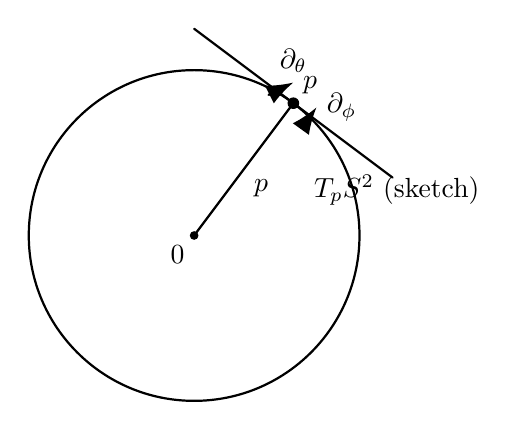
\begin{tikzpicture}[scale=1.05, line cap=round, line join=round]
			
			% Sphere as a circle (2D sketch)
			\draw[thick] (0,0) circle (2);
			
			% A point p on the sphere
			\coordinate (P) at (1.2,1.6); % roughly on the circle
			\fill (P) circle (2pt) node[above right] {$p$};
			
			% Radius vector
			\draw[thick] (0,0) -- (P) node[midway, below right] {$p$};
			
			% Tangent line at p (perpendicular to radius in this 2D sketch)
			% Tangent direction is perpendicular to OP; approximate slope
			\draw[thick] ($(P)+(-1.2,0.9)$) -- ($(P)+(1.2,-0.9)$);
			\node at ($(P)+(1.25,-1.05)$) {$T_pS^2$ (sketch)};
			
			% Small arrows indicating coordinate curves (conceptual)
			\draw[->, thick] ($(P)+(-0.3,0.1)$) -- ($(P)+(0.0,0.25)$) node[above] {$\partial_\theta$};
			\draw[->, thick] ($(P)+(0.1,-0.3)$) -- ($(P)+(0.28,-0.05)$) node[right] {$\partial_\phi$};
			
			% Center
			\fill (0,0) circle (1.5pt) node[below left] {$0$};
			
		\end{tikzpicture}
		\caption{Conceptual picture: a point $p\in S^2$, the radius vector, and the tangent plane $T_pS^2$ (drawn as a tangent line in 2D).}
	\end{figure}
	
	% ------------------------------------------------------------
	% TikZ chart 2: stereographic projection sketch
	% ------------------------------------------------------------
	\begin{figure}[H]
		\centering
		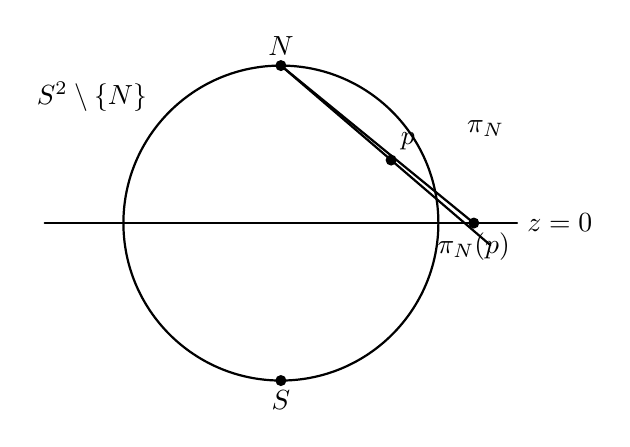
\begin{tikzpicture}[scale=1.0, line cap=round, line join=round]
			
			% Sphere as circle
			\draw[thick] (0,0) circle (2);
			
			% North and South poles
			\coordinate (N) at (0,2);
			\coordinate (S) at (0,-2);
			\fill (N) circle (2pt) node[above] {$N$};
			\fill (S) circle (2pt) node[below] {$S$};
			
			% Equatorial plane line z=0 shown as horizontal line through center
			\draw[thick] (-3,0) -- (3,0) node[right] {$z=0$};
			
			% Point p on sphere (not north)
			\coordinate (P2) at (1.4,0.8);
			\fill (P2) circle (2pt) node[above right] {$p$};
			
			% Line from North pole through p hitting plane z=0
			\draw[thick] (N) -- ($(N)!1.9!(P2)$);
			
			% Intersection with z=0 (compute by visual choice)
			\coordinate (Q) at (2.45,0);
			\fill (Q) circle (2pt) node[below] {$\pi_N(p)$};
			
			% Connect N to projection point
			\draw[thick] (N) -- (Q);
			
			% Labels
			\node at (2.6,1.2) {$\pi_N$};
			\node at (-2.4,1.6) {$S^2\setminus\{N\}$};
			
		\end{tikzpicture}
		\caption{Stereographic projection from the north pole $N$: a chart $\pi_N:S^2\setminus\{N\}\to\mathbb{R}^2$ (plane $z=0$).}
	\end{figure}
	
	\begin{figure}[H]
		\centering
		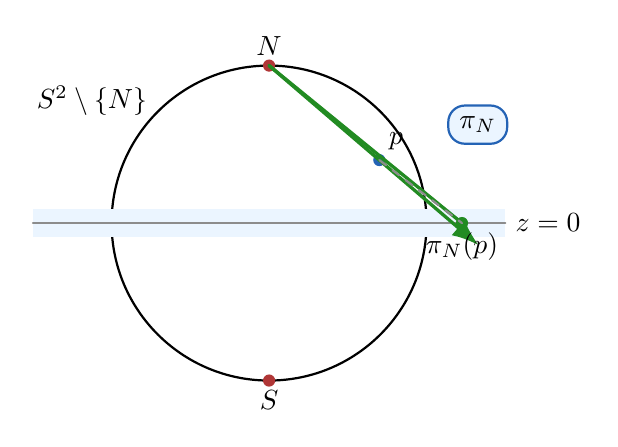
\begin{tikzpicture}[scale=1.0, line cap=round, line join=round]
			
			% ---- Colors ----
			\definecolor{blueA}{RGB}{36,99,181}
			\definecolor{redA}{RGB}{176,54,54}
			\definecolor{greenA}{RGB}{34,139,34}
			\definecolor{grayA}{RGB}{140,140,140}
			\definecolor{fillPlane}{RGB}{235,245,255}
			
			% ---- Sphere (2D sketch) ----
			\draw[thick] (0,0) circle (2);
			
			% ---- Equatorial plane z=0 (shown as a line) ----
			\fill[fillPlane] (-3,-0.18) rectangle (3,0.18); % a thin band to suggest the plane
			\draw[thick, draw=grayA] (-3,0) -- (3,0) node[right, black] {$z=0$};
			
			% ---- Poles ----
			\coordinate (N) at (0,2);
			\coordinate (S) at (0,-2);
			\fill[redA] (N) circle (2.2pt) node[above, black] {$N$};
			\fill[redA] (S) circle (2.2pt) node[below, black] {$S$};
			
			% ---- A point p on sphere (not north pole) ----
			\coordinate (P2) at (1.4,0.8);
			\fill[blueA] (P2) circle (2.2pt) node[above right, black] {$p$};
			
			% ---- Projection ray from N through p ----
			\draw[very thick, draw=greenA, ->] (N) -- ($(N)!1.9!(P2)$);
			
			% ---- Intersection point in the plane (chosen visually) ----
			\coordinate (Q) at (2.45,0);
			\fill[greenA] (Q) circle (2.2pt) node[below, black] {$\pi_N(p)$};
			
			% ---- Connect N to the projected point (same ray, emphasized) ----
			\draw[very thick, draw=greenA] (N) -- (Q);
			
			% ---- Optional helper: mark the line segment from p to Q as dashed (visual aid) ----
			\draw[thick, draw=grayA, dashed] (P2) -- (Q);
			
			% ---- Labels ----
			\node[draw=blueA, rounded corners=6pt, thick, inner sep=4pt, fill=fillPlane]
			at (2.65,1.25) {$\pi_N$};
			\node at (-2.25,1.55) {$S^2\setminus\{N\}$};
			
		\end{tikzpicture}
		\caption{Stereographic projection from the north pole $N$: the chart $\pi_N:S^2\setminus\{N\}\to\mathbb{R}^2$ (target plane $z=0$).}
	\end{figure}
	
	
	\subsection*{Problem 8: Antipodal map, orientability of real projective space, and top de Rham cohomology}
	\begin{enumerate}
		\item[(a)] For which $n$ is the antipodal map $\alpha: S^n \to S^n$ orientation-preserving?
		\item[(b)] By considering a natural $2:1$ map $\pi: S^n \to \mathbb{RP}^n$, deduce the values of $n$ for which
		$\mathbb{RP}^n$ is orientable. You may assume without proof that $\pi$ is locally a diffeomorphism.
		\item[(c)] By combining these ideas with Q5 and Q7, compute $H^n_{\mathrm{dR}}(\mathbb{RP}^n)$ for all $n$.
	\end{enumerate}
	
	\subsection*{Problem 9: Green's theorem via Stokes' theorem (pullback of a 1-form)}
	Let $\Sigma$ be a compact $2$-manifold-with-boundary, let $F : \Sigma \to \mathbb{R}^2$ be a smooth map,
	and let $\alpha$ be the $1$-form $P\,dx + Q\,dy$ on $\mathbb{R}^2$ (where $P$ and $Q$ are smooth functions).
	Prove a version of Green's theorem by applying Stokes to $F^{*}\alpha$.
	
	
	\end{document}
